
\chapter{平坦性}
\label{ch:flatness}

\epigraph{平坦性的概念是自代数中诞生的一个谜，然而在技术上，它却是对许多祈祷的回应。}{——D.~\trMumford，[Mu7, III.~10]}

我们回到\trFlatness{}这个重要概念。其实早在讨论\trQCSheaf{}与\trMorphism{}之时，我们就可以大谈平坦性了。但这是一个出人意料的想法，其代数与几何两面又看不出明显的联系，所以我们把它留到了相对靠后的地方。\trSerre{}曾说，他在其里程碑式的「GAGA」论文 [Se3] 中引入平坦性纯粹是出于代数上的理由，而认识到其几何意义的人则是\trGrothendieck。「正合」看起来似乎比「平坦」更富描述性（那样我们就会有「正合模」与「正合态射」），但这个叫法并未流行开来。

\textbf{24.0.1.}\quad \trFlat{}\trMorphism{}正是「好的」或「变化良好」的 $Y$ 上\trFamily{}这一概念的不二之选。例如，若 $\pi$ 是连通\trNoether{}基上的射影平坦族（释读：$\pi\colon X\to Y$ 是射影平坦\trMorphism，其中 $Y$ 连通且\trNoether），我们将看到纤维的各种数值不变量都是常数，包括维数（\S24.5.5），以及可以用\trEulerCharacteristic{}来解读的诸数（见 \S24.7）：
（a）\trHilbertPolynomial（\mbox{推论~24.7.2}）；
（b）（射影空间中的）次数（\mbox{练习~24.7.A}(a)）；
（\(b'\)）（作为 (b) 的特例）若 $\pi$ 有限，$\pi$ 的次数（恢复并推广「正则曲线之间射影映射的次数是常数」这一事实，\S16.3.4；见\mbox{练习~24.3.G} 与 \S24.3.12）；
（c）\trArithmeticGenus\footnote{原书此处作「\mbox{练习~24.7.A}(b)」，惟 \mbox{练习~24.7.A} 实列 (a) 纤维次数、(b) 纤维维数、(c) \trArithmeticGenus，当为「(c)」之误，径改。——译者注}（\mbox{练习~24.7.A}(c)）；
（d）纤维为\trCurve{}时\trLineBundle{}的次数（\mbox{推论~24.7.3}）；
（e）\trDivisor{}与\trLineBundle{}的相交（\mbox{练习~24.7.D}）。

你可能以为合适的假设该是\trSmoothness，或者更一般地，某种等奇异性，但我们只需要更弱的条件。而这是件好事：\trBranchedCover{}在任何传统意义下都不是纤维化，却依然表现良好——由 $y\mapsto x^2$ 给出的二重覆盖 $\mathbb{A}^1\to\mathbb{A}^1$ 有常次数 $2$（\S10.3.4，\S16.3.10 再访）。另一个关键例子，是一族光滑曲线退化成结点曲线的\trFamily（图~\ref{fig:flat-nodal-degeneration}）——（底层解析）曲线的拓扑变了，但\trArithmeticGenus{}保持恒常。关于正则曲线的命题可以这样证明：先对结点退化证明之，再证明该结果在平坦\trFamily{}中表现良好。这类退化技术在代数几何中无处不在。

\begin{figure}[htbp]
\centering
\begin{tikzpicture}[scale=0.9,line width=0.8pt]
  \draw (1.15,0.2) .. controls (0.35,0.9) and (0.35,2.1) .. (1.15,2.8);
  \draw (2.75,0.0) .. controls (2.15,0.8) and (2.5,2.0) .. (3.45,2.75)
        .. controls (3.85,3.0) and (4.05,2.6) .. (3.85,2.25)
        .. controls (3.6,1.8) and (2.85,1.5) .. (2.95,1.0)
        .. controls (3.05,0.55) and (3.6,0.45) .. (3.9,0.0);
  \draw (5.05,1.5) circle (0.22);
  \draw (6.35,0.2) .. controls (5.55,0.9) and (5.55,2.1) .. (6.35,2.8);
  \draw[gray!75,->] (3.25,-0.45) -- (3.25,-1.5);
  \draw (0.9,-1.85) -- (6.6,-1.85);
  \fill (3.25,-1.85) circle (2pt);
  \node at (3.25,-2.45) {$t=0$};
  \node at (8.15,-1.85) {$\mathbb{A}^1_k=\Spec k[t]$};
\end{tikzpicture}
\caption{一个平坦\trFamily：光滑曲线退化成结点曲线：$y^2=x^3+x^2+tx$。（依原书手绘图重绘。）}\label{fig:flat-nodal-degeneration}
\end{figure}

鉴于「欧拉示性数恒常」这一定理的上同调本性，你不必惊讶所需的假设（平坦性）也是上同调本性的——它可以用 $\mathrm{Tor}$ 的消失来刻画（\mbox{练习~23.1.C}），我们将在 \S24.2 中把它用得淋漓尽致。

但平坦性还有其他方面的重要性。首先：既然它是「好\trFamily」的正确概念，它使我们能够正确地定义\trModuliSpace{}的概念。例如，$\mathbb{P}^n$ 的\emph{\trHilbertScheme}（Hilbert scheme）「参数化了 $\mathbb{P}^n$ 的诸闭子概形」。从概形 $B$ 到\trHilbertScheme{}的态射，相应于 $\mathbb{P}^n_B$ 上平坦于 $B$ 的（有限表现的）闭子概形。由泛性质的废话，这就在相差唯一\trIsomorphism{}的意义下定义了\trHilbertScheme（当然我们还必须证明它存在，这颇费一番功夫——更多内容见\mbox{定理~25.3.1}）。光滑射影曲线的\trModuliSpace{}则由这样一条\trUniversalProperty{}定义：到该\trModuliSpace{}的态射，相应于几何纤维皆为光滑曲线的射影平坦（有限表现）\trFamily。（遗憾的是，这个\trModuliSpace{}并不存在。）与此相关，平坦性在\trDeformationTheory{}中处于核心地位：它是理解概形（以及其他几何对象，比如向量丛）如何\trDeformation{}的关键（参看 \S21.5.12）。最后，\trGalois{}下降的概念推广为（忠实）「\trFlat{}下降」，使我们能够像在\trZariskiTopology{}（或更经典的拓扑）中那样，在更为新奇的\trGrothendieck{}拓扑中「粘合」；但这超出了我们当前讨论的范围。

平坦性有许多风味各异的面向，很容易只见树木、不见森林。由于平坦性的代数看起来与几何如此不相关，它可能并不直观。我们将不可避免地从代数基础开始，但你应该聚焦于以下几点：证明事物平坦的方法（既有一般判别法也有显式例子），以及特定类型的环上平坦模的分类。凡是涉及这类显式例子的练习，你都应当亲手做一做。

以下是本章的概要，以帮助你聚焦注意力。
\begin{itemize}
\item 在 \S24.1 中，我们讨论一些较为容易的事实，它们本质上是代数性的。
\item \S24.2、\S24.3 与 \S24.6 给出平坦性的理想论判别法。\S24.2 与 \S24.3 应当连在一起读。前者用 $\mathrm{Tor}$ 来理解平坦性，后者则利用这些洞见发展出平坦性的理想论判别法。\S24.6 讲平坦性的局部判别法，较难。
\item \S24.5 相对独立，可以在 \S24.1 之后立即阅读。它讨论平坦性的拓扑面向，比如「在好的情形中，平坦态射是开映射」这一事实。（回想：拓扑空间之间的映射称作\trOpenMap，如果每个开集的像都是开集。）
\item 在 \S24.7 中，我们解释「拟凝聚层的\trEulerCharacteristic{}在平坦\trFamily{}中是常数」（在适当假设下）这一事实，以及它带来的许多可喜推论。鉴于其用处，这一节出奇地容易。
\end{itemize}

你应当聚焦于平坦性蕴含什么、如何把它「画出来」，但也要聚焦于不同情形下平坦性的显式判别法，比如：\trIntegralDomain（\mbox{观察~24.1.2}）、\trPID（\mbox{练习~24.3.B}）、\trDVR（\mbox{练习~24.3.C}）、\trDualNumbers（\mbox{练习~24.3.D}）、局部环（\mbox{定理~24.3.5}）。


\section{较容易的事实}

\epigraph{幸福的家庭彼此相似；每个不幸福的家庭各有其不幸福。（例如参看图~\ref{fig:not-flat-morphisms}，以及\mbox{练习~24.1.G}(d)、\mbox{练习~24.1.L} 与 \mbox{练习~24.3.H}。）}{——L.~\trTolstoy，《安娜·卡列尼娜》，[To, l.~1]}

关于平坦性的许多事实是容易的、或是随即可得的，虽然其中也有一些颇为棘手。一如既往，我会尽力分清何者为何，以帮助你记住容易的事实，以及较难事实的证明之关键想法。我们先摘低垂的果实。

我们回想一下平坦 $A$-\trModule{}的定义（\S1.5.13）。若 $M\in\mathit{Mod}_A$，则 $M\otimes_A\cdot$ 总是\trRightExact{}的（\mbox{练习~1.2.H}）。我们说 $M$ 是一个\textbf{平坦 $A$-\trModule}（或\emph{在 $A$ 上平坦}，或\emph{$A$-平坦}），如果 $M\otimes_A\cdot$ 是一个\trExact{}函子。我们说\trRingMorphism{} $B\to A$ 是\textbf{平坦}的，如果 $A$ 作为 $B$-\trModule{}是平坦的。（特别地，这与 $A$ 的代数结构无关。）

\textbf{24.1.1.}\ \emph{两个关键例子。}\quad
（i）自由 $A$-\trModule{}（哪怕是无限秩的）显然是平坦的。更一般地，\trProjectiveObj{}\trModule{}是平坦的（\mbox{练习~23.2.B}）。

（ii）局部化是平坦的：设 $S$ 是 $B$ 的一个\trMultiplicativeSubset。则 $B\to S^{-1}B$ 是平坦的\trRingMorphism，因为局部化是正合的（\mbox{练习~1.5.G}(a)）。

\textbf{24.1.A.（容易练习：最初的例子）}\quad
（a）（\emph{陷阱问题}）对\trField{} $k$ 上的平坦\trModule{}进行分类。
（b）证明 $A[x_1,\dots,x_n]$ 是平坦的 $A$-\trModule。
（c）证明\trRingMorphism{} $\mathbb{Q}[x]\to\mathbb{Q}[y]$（$x\mapsto y^{2}$）是平坦的。（这将帮助我们更好地理解\mbox{例~10.3.4}；见 \S24.3.12。）

我们来作几条快速而重要的观察。

\textbf{24.1.2.}\ \emph{重要观察。}\quad 若 $x$ 是 $A$ 的一个\trNonZerodivisor，而 $M$ 是平坦的 $A$-\trModule，则
\[
M \xrightarrow{\ \times x\ } M
\]
是\trInjectiveMap{}的。（把\trExact{}函子 $M\otimes_A\cdot$ 作用到正合列 $0\longrightarrow A\xrightarrow{\ \times x\ }A$ 上。）特别地，\emph{平坦\trModule{}都\trTorsionFree}。（\trTorsionFree{}性定义于 \S6.1.4。）这条观察给出了一个简便的办法，让我们能识别出一个\trModule{}何时不\trFlat；我们将会多次用到它。

\textbf{24.1.B.（练习：另一个例子）}\quad 证明：\trPID{}上\trFinitelyGenerated{}的\trModule{}是平坦的，当且仅当它\trTorsionFree，当且仅当它是自由的。提示：\mbox{注记~6.4.4} 对\trPID{}上有限生成的\trModule{}作了分类。（\mbox{练习~24.3.B} 将进一步阐明\trPID{}上的平坦性。\mbox{命题~14.3.2} 亦与之相关。）

\textbf{24.1.C.（练习：平坦性在更换基环下保持）}\quad 证明：若 $M$ 是平坦的 $B$-\trModule，而 $B\to A$ 是一个\trHomomorphism，则 $M\otimes_B A$ 是平坦的 $A$-\trModule。

\textbf{24.1.D.（练习：平坦性在复合下保持）}\quad 证明：若 $A$ 是平坦的 $B$-\trAlgebra，而 $M$ 是 $A$-平坦的，则 $M$ 也是 $B$-平坦的。

\textbf{24.1.3. \trhProposition{}（平坦性是茎／素局部性质）。}\ ——\ \emph{一个 $A$-\trModule{} $M$ 是\trFlat{}的，当且仅当对一切\trPrimeIdeal{} $\mathfrak{p}\subset A$，$M_{\mathfrak{p}}$ 都是平坦的 $A_{\mathfrak{p}}$-\trModule。}

欢迎你去证明其实只须检验\emph{极大}理想即可，但我们并不需要这一扩展。

\emph{证明。}\quad 先设 $M$ 是平坦的 $A$-\trModule。给定任意一个 $A_{\mathfrak{p}}$-\trModule{}的正合列
\[
\tag{24.1.3.1}\label{eq:flat-stalk-ses}
0 \longrightarrow N' \longrightarrow N \longrightarrow N'' \longrightarrow 0,
\]
我们希望证明
\[
\tag{24.1.3.2}\label{eq:flat-stalk-tensor}
0 \longrightarrow M_{\mathfrak{p}}\otimes_{A_{\mathfrak{p}}} N' \longrightarrow M_{\mathfrak{p}}\otimes_{A_{\mathfrak{p}}} N \longrightarrow M_{\mathfrak{p}}\otimes_{A_{\mathfrak{p}}} N'' \longrightarrow 0
\]
也正合。而 \eqref{eq:flat-stalk-ses} \emph{同时}也是 $A$-\trModule{}的正合列，故
\[
\tag{24.1.3.3}\label{eq:flat-global-tensor}
0 \longrightarrow M\otimes_A N' \longrightarrow M\otimes_A N \longrightarrow M\otimes_A N'' \longrightarrow 0
\]
是正合的（由 $M$ 的 $A$-平坦性）。但 $M\otimes_A N$ \trCanonical{}同构于 $M\otimes_A A_{\mathfrak{p}}\otimes_{A_{\mathfrak{p}}}N=M_{\mathfrak{p}}\otimes_{A_{\mathfrak{p}}}N$（$N'$ 与 $N''$ 同理），于是我们可以把 \eqref{eq:flat-global-tensor} 改写成 \eqref{eq:flat-stalk-tensor}（务必看清 \eqref{eq:flat-global-tensor} 与 \eqref{eq:flat-stalk-tensor} 中的映射为何是相同的），此即所欲证。

再设对一切 $\mathfrak{p}$，$M_{\mathfrak{p}}$ 都是平坦的 $A_{\mathfrak{p}}$-\trModule。给定任意\trShortExactSequence{} \eqref{eq:flat-stalk-ses}，我们要证 \eqref{eq:flat-global-tensor} 正合。由张量积的\trRightExact{}性（\mbox{练习~1.2.H}），除了可能在左端失准之外，\eqref{eq:flat-global-tensor} 是正合的。令 $K$ 为 $\ker(M\otimes_A N'\to M\otimes_A N)$，于是
\[
\tag{24.1.3.4}\label{eq:flat-kernel-ses}
0 \longrightarrow K \longrightarrow M\otimes_A N' \longrightarrow M\otimes_A N \longrightarrow M\otimes_A N'' \longrightarrow 0
\]
正合；我们希望证明 $K=0$。任取 $\mathfrak{p}$，把 \eqref{eq:flat-stalk-ses} 在 $\mathfrak{p}$ 处局部化，再与正合的 $A_{\mathfrak{p}}$-\trModule{} $M_{\mathfrak{p}}$ 作张量，便得
\[
\tag{24.1.3.5}\label{eq:flat-local-tensor}
0 \longrightarrow M_{\mathfrak{p}}\otimes_{A_{\mathfrak{p}}} N'_{\mathfrak{p}} \longrightarrow M_{\mathfrak{p}}\otimes_{A_{\mathfrak{p}}} N_{\mathfrak{p}} \longrightarrow M_{\mathfrak{p}}\otimes_{A_{\mathfrak{p}}} N''_{\mathfrak{p}} \longrightarrow 0.
\]
把 \eqref{eq:flat-kernel-ses} 在 $\mathfrak{p}$ 处局部化，并利用诸同构 $M_{\mathfrak{p}}\otimes_{A_{\mathfrak{p}}}N_{\mathfrak{p}}\overset{\sim}{\longleftrightarrow}(M\otimes_A N)_{\mathfrak{p}}$，我们得到正合列
\[
0 \longrightarrow K_{\mathfrak{p}} \longrightarrow M_{\mathfrak{p}}\otimes_{A_{\mathfrak{p}}} N'_{\mathfrak{p}} \longrightarrow M_{\mathfrak{p}}\otimes_{A_{\mathfrak{p}}} N_{\mathfrak{p}} \longrightarrow M_{\mathfrak{p}}\otimes_{A_{\mathfrak{p}}} N''_{\mathfrak{p}} \longrightarrow 0,
\]
它与正合列 \eqref{eq:flat-local-tensor} 完全相同，只是多出了 $K_{\mathfrak{p}}$。于是对一切素理想 $\mathfrak{p}\subset A$ 都有 $K_{\mathfrak{p}}=0$，从而 $K=0$（由\mbox{练习~4.1.F}），此即所欲证。\hfill$\square$

\textbf{24.1.4. 概形上的平坦性。}\quad 受\mbox{命题~24.1.3} 的推动，把平坦性的概念推广到概形上是直截了当的。

\textbf{24.1.5. \trhDefinition{}：平坦拟凝聚层。}\quad 我们说概形 $X$ 上的一个\trQCSheaf{} $\mathscr{F}$ \textbf{在 $\mathfrak{p}\in X$ 处平坦}，如果 $\mathscr{F}_{\mathfrak{p}}$ 是平坦的 $\OO_{X,\mathfrak{p}}$-\trModule。我们说概形 $X$ 上的一个\trQCSheaf{} $\mathscr{F}$ 是\textbf{平坦}的（于 $X$ 上），如果它在所有 $\mathfrak{p}\in X$ 处都平坦。鉴于\mbox{命题~24.1.3}，我们可以在 $X$ 的一个\trAffine\trOpenCover{}上检验这个概念。

\textbf{24.1.6. \trhDefinition{}：平坦\trMorphism。}\quad 类似地，我们说概形之间的\trMorphism{} $\pi\colon X\to Y$ \textbf{在 $\mathfrak{p}\in X$ 处平坦}，如果 $\OO_{X,\mathfrak{p}}$ 是平坦的 $\OO_{Y,\pi(\mathfrak{p})}$-\trModule。我们说概形之间的\trMorphism{} $\pi\colon X\to Y$ 是\textbf{平坦}的，如果它在所有 $\mathfrak{p}\in X$ 处都平坦。我们可以在源与靶上局部地检验平坦性。

我们可以把这两条定义合并成单条花哨的定义。

\textbf{24.1.7. \trhDefinition{}：基上的平坦拟凝聚层。}\quad 设 $\pi\colon X\to Y$ 是概形之间的一个\trMorphism，而 $\mathscr{F}$ 是 $X$ 上的一个\trQCSheaf。我们说 $\mathscr{F}$ \textbf{在 $\mathfrak{p}\in X$ 处平坦（于 $Y$ 上）}，如果 $\mathscr{F}_{\mathfrak{p}}$ 是平坦的 $\OO_{Y,\pi(\mathfrak{p})}$-\trModule。我们说 $\mathscr{F}$ \textbf{是平坦的（于 $Y$ 上）}，如果它在所有 $\mathfrak{p}\in X$ 处都平坦。

\mbox{定义~24.1.5} 与 \mbox{定义~24.1.6} 分别对应于 $X=Y$ 与 $\mathscr{F}=\OO_X$ 的情形。（\mbox{定义~24.1.7} 可不加改动地适用于\trRingedSpace{}的范畴，但我们不会用到这一点。）

\textbf{24.1.E.（容易练习（现实检验））}\quad 证明：\trOpenEmbedding{}都是平坦的。

我们上文关于环上平坦性的诸结果可以轻易地搬到概形上。

\textbf{24.1.F.（练习）}\quad 证明：环映射 $B\to A$ 是平坦的，当且仅当相应的概形\trMorphism{} $\Spec A\to\Spec B$ 是平坦的。更一般地，若 $B\to A$ 是一个环映射，而 $M$ 是一个 $A$-\trModule，证明 $M$ 是 $B$-平坦的，当且仅当 $\widetilde{M}$ 在 $\Spec B$ 上平坦。（要当心：这需要的可不只是简单地援引\mbox{命题~24.1.3}。）提示：在两个方向上都用间接的方式入手是一条好路子。「假设 $M_{\mathfrak{p}}$ 不是 $B_{\mathfrak{p}}$-平坦的。\footnote{译注：原书此处作「$M_{\mathfrak{p}}$ 不是 $B_{\mathfrak{q}}$-平坦的」，当为「$B_{\mathfrak{p}}$」之误，径改。——译者注}那么存在 $B_{\mathfrak{p}}$-\trModule{}（从而也是 $B$-\trModule{}）的一个正合列 $0\to N'\to N\to N''\to 0$，使得……。」「假设 $\widetilde{M}$ 不是 $B$-平坦的。那么存在 $B$-\trModule{}的一个正合列……。」

于是，若 $\pi\colon X\to Y$ 是\trAffine\trMorphism，而 $\mathscr{F}$ 是 $X$ 上的一个\trQCSheaf，则 $\mathscr{F}$ 在 $Y$ 上平坦，当且仅当 $\pi_\ast\mathscr{F}$ 在 $Y$ 上平坦。

\textbf{24.1.G.（容易练习（例子与现实检验））}\quad
（a）设 $X$ 是概形，而 $\mathfrak{p}\in X$，证明自然\trMorphism{} $\Spec\OO_{X,\mathfrak{p}}\to X$ 是平坦的。（提示：局部化是平坦的，\S24.1.1。）
（b）证明 $\mathbb{A}^{n}_A\to\Spec A$ 是平坦的。
（c）若 $\mathscr{F}$ 是概形 $X$ 上的一个\trLocallyFreeSheaf，证明 $\mathbb{P}\mathscr{F}\to X$（\mbox{定义~17.2.4}）是平坦的。
（d）证明 $\Spec k\to\Spec k[t]/(t^{2})$ 不平坦。（画一张图，试着看出这个\trMorphism{}有什么地方不「好」。关于\trDualNumbers{}之平坦性的更多洞见，将在\mbox{练习~24.3.D} 的判别法中给出。）

\textbf{24.1.H.（练习）}\quad 证明：若 $\pi\colon X\to Y$ 是平坦\trMorphism，则 $\pi^{*}\colon\mathit{QCoh}_Y\to\mathit{QCoh}_X$ 是一个\trExact{}函子。

\textbf{24.1.I.（练习：平坦性在复合下保持）}\quad 设 $\pi\colon X\to Y$，而 $\mathscr{F}$ 是 $X$ 上的一个在 $Y$ 上平坦的\trQCSheaf。再设 $\psi\colon Y\to Z$ 是平坦\trMorphism。证明 $\mathscr{F}$ 在 $Z$ 上平坦。

\textbf{24.1.J.（练习：平坦性在基变换下保持）}\quad 设 $\pi\colon X\to Y$ 是一个\trMorphism，而 $\mathscr{F}$ 是 $X$ 上的一个在 $Y$ 上平坦的\trQCSheaf。若 $\rho\colon Y'\to Y$ 是任意\trMorphism，而 $\rho'\colon X\times_Y Y'\to X$ 是由此诱导的\trMorphism，证明 $(\rho')^{*}\mathscr{F}$ 在 $Y'$ 上平坦。
\[
\begin{tikzcd}[row sep=2.6em, column sep=2.6em]
(\rho')^{*}\mathscr{F} \ar[d] & \mathscr{F} \ar[d] \\
X\times_Y Y' \ar[r, "\rho'"] \ar[d] & X \ar[d, "\pi"] \\
Y' \ar[r, "\rho"] & Y
\end{tikzcd}
\]
特别地，利用\mbox{练习~24.1.A}(a)，若 $Y=\Spec k$（而 $X$ 与 $Y'$ 是\emph{任意}的 $k$-概形，$\mathscr{F}$ 是 $X$ 上\emph{任意}的\trQCSheaf），则 $(\rho')^{*}\mathscr{F}$ 在 $Y'$ 上平坦。例如，$X\times_k Y'$ 总是在 $Y'$ 上平坦的——「域上的乘积平坦于其各因子」。（欢迎立刻把它进一步推广；例如，$\mathscr{F}$ 可以是概形 $Z\to X$ 上的一个\trQCSheaf，在 $Y$ 上平坦。）

\textbf{24.1.8.}\ \emph{平坦\trMorphism{}表现合理。}\quad 由定义，平坦性显然在靶上是局部的，于是前两道练习表明：平坦\trMorphism{}这个类在 \S8.1 的意义下是「\trReasonable」的。

下面这道练习对于将平坦与非平坦可视化极为有用（例如参看图~\ref{fig:not-flat-morphisms}）。

\textbf{24.1.K.（练习：平坦映射把相伴点送到相伴点）}\quad 设 $\pi\colon X\to Y$ 是\trLocally\trNoether{}概形之间的一个平坦\trMorphism。证明 $X$ 的任何\trAssociatedPoint{}都必定被映到 $Y$ 的一个\trAssociatedPoint。（欢迎立刻把它推广到 $X$ 上一个在 $Y$ 上平坦的凝聚层 $\mathscr{F}$，而 $\pi$ 本身不必平坦。）提示：设 $\pi^{\sharp}\colon(B,\mathfrak{n})\to(A,\mathfrak{m})$ 是\trNoether{}局部环之间的一个局部态射（即 $\pi^{\sharp}(\mathfrak{n})\subset\mathfrak{m}$，\S7.3.1）。设 $\mathfrak{n}$ 不是 $B$ 的\trAssociatedPrimeIdeal。证明存在一个元素 $f\in\mathfrak{n}$ 不属于 $B$ 的任何\trAssociatedPrimeIdeal（或许可以借助\trPrimeIdeal{}回避，\mbox{命题~12.2.13}），从而它是\trNonZerodivisor。利用\mbox{观察~24.1.2} 证明 $\pi^{\sharp}f\in\mathfrak{m}$ 是 $A$ 的\trNonZerodivisor，从而证明 $\mathfrak{m}$ 不是 $A$ 的\trAssociatedPrimeIdeal。

\textbf{24.1.L.（练习）}\quad 利用\mbox{练习~24.1.K} 证明：以下诸\trMorphism{}都不平坦（参看图~\ref{fig:not-flat-morphisms}）：
（a）$\Spec k[x,y]/(xy)\to\Spec k[x]$；
（b）$\Spec k[x,y]/(y^{2},xy)\to\Spec k[x]$；
（c）$\mathrm{Bl}_{(0,0)}\mathbb{A}^{2}_k\to\mathbb{A}^{2}_k$。
（c）的提示：先拉回到过原点的一条直线上，得到一个与 (a) 相仿的东西。\footnote{译注：原书此处作「to obtain a something akin to (a)」，当为「to obtain something akin to (a)」之误，径改。——译者注}（这预示了\mbox{命题~24.5.6} 的陈述与证明，该命题断言：对于平坦\trMorphism{}，「纤维维数不会跳变」。）

\begin{figure}[htbp]
\centering
\begin{tikzpicture}[scale=0.85, line width=0.8pt]
  \draw (0.2,0) -- (1.8,0);
  \draw (1.0,-0.75) -- (1.0,0.75);
  \draw[gray!70,->] (1.0,-1.15) -- (1.0,-2.05);
  \draw (0.2,-2.55) -- (1.8,-2.55);
  \node at (1.0,-3.25) {(a)};
  \draw (2.7,0) -- (4.3,0);
  \fill[gray!80] (3.25,0) circle (2.6pt);
  \draw[gray!70,->] (3.5,-1.15) -- (3.5,-2.05);
  \draw (2.7,-2.55) -- (4.3,-2.55);
  \node at (3.5,-3.25) {(b)};
  \begin{scope}[shift={(5.4,0)}]
    \draw (0.35,0.55) -- (2.2,0.55) -- (1.55,-0.65) -- (-0.3,-0.65) -- cycle;
    \draw (1.15,-0.3) -- (1.15,0.3);
    \node at (1.4,0.05) {$\mathrm{E}$};
    \draw[gray!70,->] (0.85,-1.05) -- (0.85,-2.0);
    \node at (1.9,-1.55) {胀开};
    \draw (0.35,-3.15) -- (2.2,-3.15) -- (1.55,-4.35) -- (-0.3,-4.35) -- cycle;
    \fill (0.95,-3.75) circle (1.8pt);
    \node at (0.95,-5.0) {(c)};
  \end{scope}
\end{tikzpicture}
\caption{不平坦的\trMorphism{}（\mbox{练习~24.1.L}）。（依原书手绘图重绘。）}\label{fig:not-flat-morphisms}
\end{figure}

\textbf{24.1.9. \trhTheorem{}（上同调与平坦基变换交换）。}\ ——\ \emph{设}
\[
\begin{tikzcd}[row sep=2.4em, column sep=2.6em]
X' \ar[r, "\rho'"] \ar[d, "\pi'"] & X \ar[d, "\pi"] \\
Y' \ar[r, "\rho"] & Y
\end{tikzcd}
\]
\emph{是一个\trCartesianDiagram，且 $\pi$（从而 $\pi'$）\trQuasicompact{}且\trSeparated（于是 $\pi$ 与 $\pi'$ 对\trQCSheaf{}的\trHigherPushforward{}存在，如 \S18.7 中所述）。再设 $\rho$ 是平坦的，而 $\mathscr{F}$ 是 $X$ 上的一个\trQCSheaf。那么，自然「推拉」态射（\mbox{练习~18.7.B}(a)）$\rho_{*}(\mathrm{R}^{i}\pi_\ast\mathscr{F})\to\mathrm{R}^{i}\pi'_\ast(\rho'^{*}\mathscr{F})$ 都是\trIsomorphism。}

\textbf{24.1.M.（练习）}\quad 证明\mbox{定理~24.1.9}。提示：\mbox{练习~18.7.B}(b) 是 $\rho$ 为\trAffine{}时的特例。利用与\mbox{练习~14.4.C} 的解答（其中用到了\mbox{练习~6.2.G}）相同的想法，把它推广到\trQuasicompact{}且\trSeparated{}的情形。你对 $i=0$ 情形的证明只须将「分离」假设换成「拟分离」假设即可。

一个有用的特例：取 $Y'$ 为 $Y$ 某个\trReduced{}分量的\trGenericPoint。换句话说，由\mbox{练习~24.1.G}(a)，$\mathscr{F}$ 的\trHigherPushforward{}在\trGenericPoint{}处的\trStalk，就是 $\mathscr{F}$ 在\trGenericPoint{}之上纤维上的上同调。这是某件重要事情的第一例：用\trHigherPushforward{}来理解纤维上（的\trQCSheaf）的上同调。（我们当然希望\trHigherPushforward{}能告诉我们一些关于纤维高阶上同调的事情，但这先验地绝不显然！）这条结果表明\emph{任何}\trQCSheaf{}的上同调都与\emph{平坦}基变换交换；与之相比，\S24.7 与第 25 章讨论的则是：\emph{平坦}\trQCSheaf{}的上同调何时以及如何与\emph{任何}基变换交换。

\textbf{24.1.10. 用平坦\trMorphism{}拉回\trClosedSubscheme{}（与\trIdealSheaf）。}\quad \trClosedSubscheme{}在平坦\trMorphism{}下拉回得格外好，这一点值得记在心里。正如\mbox{注记~14.5.9} 所指出的，在平坦\trMorphism{}的情形，把\trIdealSheaf{}当作\trQCSheaf{}来拉回，与经由相应\trClosedSubscheme{}之拉回的表述是一致的。换句话说，闭子概形正合列在平坦拉回下被拉回（保持正合）。事实上，这不只是平坦性的一个必要条件；它也是充分的，这可以用平坦性的理想论判别法（\mbox{定理~24.3.1}）来证明。还有一个类似的事实，是关于用\emph{任意}拉回来拉回\emph{平坦}子概形的\trIdealSheaf{}的；见 \S24.2.2。

\textbf{24.1.N.（练习）}\quad
（a）设 $D$ 是 $Y$ 上的一个\trEffectiveCartierDivisor，而 $\pi\colon X\to Y$ 是平坦\trMorphism。证明 $D$ 到 $X$ 的拉回（经由 $\pi$）也是\trEffectiveCartierDivisor。
（b）利用 (a) 证明：在平坦\trMorphism{}下，\trRegularEmbedding{}拉回为\trRegularEmbedding。

\textbf{24.1.O.（练习）}\quad
（a）设 $\pi\colon X\to Y$ 是一个\trMorphism，而 $Z\hookrightarrow Y$ 是由一个\trIdealSheaf{} $\mathscr{I}\subset\OO_Y$ 切出的\trClosedEmbedding。仅限本练习：对任意对应于\trClosedSubscheme{} $W\subset Y$ 的\trIdealSheaf{} $\mathscr{J}\subset\OO_Y$，令 $\pi^{\flat}\mathscr{J}\subset\OO_X$ 记对应于 $W\times_Y X\subset X$ 的\trIdealSheaf（于是 $\pi^{*}\mathscr{J}\to\pi^{\flat}\mathscr{J}$ 是满射，但正如\mbox{注记~14.5.9} 所讨论的，它并不总是\trIsomorphism）。证明 $(\pi^{\flat}\mathscr{I})^{n}=\pi^{\flat}(\mathscr{I}^{n})$。（拟凝聚理想层的乘积定义于\mbox{练习~15.6.E}。）
（b）进而设 $\pi$ 是平坦的，$Y=\mathbb{A}^{n}_k$，而 $Z$ 是原点。令 $\mathscr{J}=\pi^{*}\mathscr{I}$ 为 $X$ 上切出 $Z$ 之拉回 $W$ 的\trQC{}\trSheafOfAlgebras。证明分次代数层 $\bigoplus_{n\ge 0}\mathscr{J}^{n}/\mathscr{J}^{n+1}$（你理解其中的乘法吗？）\trIsomorphic{}于 $\OO_W[x_1,\dots,x_n]$（解释为\trSheafOfGradedAlgebras）。（提示：先证明 $\mathscr{J}^{n}/\mathscr{J}^{n+1}\cong\Sym^{n}(\mathscr{J}/\mathscr{J}^{2})$，\mbox{推论~22.3.9}。这一思路将在\mbox{练习~24.6.E} 中得到重访。）

\textbf{24.1.P.（练习）}\quad
（a）证明：胀开与平坦基变换交换。更精确地说，若 $\pi\colon X\to Y$ 是任意平坦\trMorphism，而 $Z\hookrightarrow Y$ 是任意\trClosedEmbedding，给出典范\trIsomorphism{} $(\mathrm{Bl}_{Z}\,Y)\times_Y X\overset{\sim}{\longleftrightarrow}\mathrm{Bl}_{Z\times_Y X}\,X$。（你可以经由\trUniversalProperty、利用\mbox{练习~24.1.N}(a) 来做；或者利用胀开的 $\Proj$ 构造与\mbox{练习~24.1.O} 来做。）
（b）举出一个例子，说明胀开一般不与基变换交换。



\section{经 $\mathrm{Tor}$ 看平坦性}

我们在 \S23.1 中定义了 $\mathrm{Tor}$（双）函子：$\mathrm{Tor}^A_i(M,N)$ 的作法是取 $N$ 的一个\trFreeModule{}分解，剥掉 $N$，与 $M$ 作张量，再取\trHomology。\mbox{练习~23.1.C} 已经用 $\mathrm{Tor}$ 刻画了\trFlatness：若对一切 $N$ 都有 $\mathrm{Tor}^A_i(M,N)=0$，则 $M$ 是 $A$-\trFlat{}的。本节中，我们来收割这一刻画所带来的那些较为容易的回报，需要时顺带回顾 $\mathrm{Tor}$ 的几条关键性质。到了 \S24.3，我们会更加下力气地从 $\mathrm{Tor}$ 中榨取更多。

有时，直接从定义出发也能算出 $\mathrm{Tor}$，下面这道我们将反复用到的练习便是一例。

\textbf{24.2.A.（练习）}\quad 把 $(M:x)$ 定义为 $\{m\in M:xm=0\}\subset M$——它由 $M$ 中被 $x$ \trAnnihilate{}的那些元素组成。若 $x$ 不是\trZerodivisor，证明：
\[
\mathrm{Tor}^A_i(M,A/(x))=
\begin{cases}
M/xM & \text{若 } i=0\text{；}\\
(M:x) & \text{若 } i=1\text{；}\\
0 & \text{若 } i>1.
\end{cases}
\]
提示：用 $A/(x)$ 的如下分解：
\[
0 \longrightarrow A \overset{\times x}{\longrightarrow} A \longrightarrow A/(x) \longrightarrow 0.
\]

\textbf{24.2.1.}\ \emph{\trhRemark。}\quad 作为\mbox{练习~24.2.A} 的一个推论，我们再次看到：\trIntegralDomain{}上的\trFlat\trModule{}都\trTorsionFree（而且，更一般地，见\mbox{观察~24.1.2}）。此外，\mbox{练习~24.2.A} 也交代了记号 $\mathrm{Tor}$ 的缘由——它是 torsion（\trTorsion）的缩写。

\textbf{24.2.B.（练习）}\quad 若 $B$ 在 $A$ 上\trFlat，用 FHHF 定理（\mbox{练习~1.5.I}(c)）给出同构 $B\otimes_A\mathrm{Tor}^A_i(M,N)\overset{\sim}{\longleftarrow}\mathrm{Tor}^B_i(B\otimes M,B\otimes N)$。

回想：$\mathrm{Tor}$ 函子对其两个变元是对称的（存在同构 $\mathrm{Tor}^A_i(M,N)\overset{\sim}{\longleftarrow}\mathrm{Tor}^A_i(N,M)$，见\mbox{练习~23.3.A}）。由这条我们立得一个快捷却极为有用的结果。

\textbf{24.2.C.（容易练习）}\quad 若 $0\to N'\to N\to N''\to 0$ 是 $A$-\trModule{}的一个\trExactSequence，且 $N''$ \trFlat（例如自由），证明：对\emph{任何} $A$-\trModule{} $M$，$0\to M\otimes_A N'\to M\otimes_A N\to M\otimes_A N''\to 0$ 皆\trExact。

早在见到 $\mathrm{Tor}$ 之前，我们本来就会关心这个结果，所以它为学习 $\mathrm{Tor}$ 提供了一些动机。（不重要的旁问：不用 $\mathrm{Tor}$、只用追图，你能证明它吗？）

\textbf{24.2.D.（练习：\mbox{练习~24.2.C} 的重要推论）}\quad 设 $0\to\mathscr{F}'\to\mathscr{F}\to\mathscr{F}''\to 0$ 是\trScheme{} $Y$ 上诸\trQCSheaf{}的一个\trShortExactSequence，且 $\mathscr{F}''$ \trFlat（例如局部自由）。证明：若 $\pi\colon X\to Y$ 是概形之间的任意\trMorphism，则拉回后的序列 $0\to\pi^*\mathscr{F}'\to\pi^*\mathscr{F}\to\pi^*\mathscr{F}''\to 0$ 仍\trExact。

\textbf{24.2.E.（练习：关于\trVectorBundle{}的相应事实，参看\mbox{练习~14.2.H}）}\quad 设 $0\to M'\to M\to M''\to 0$ 是 $A$-\trModule{}的一个\trExactSequence。

（a）若 $M$ 与 $M''$ 都\trFlat，证明 $M'$ 也\trFlat。（提示：回想诸 $\mathrm{Tor}$ 的\trLongExactSequence（\mbox{命题~23.1.2}）；再利用：$N$ \trFlat{}当且仅当对一切 $i>0$ 与一切 $N'$ 都有 $\mathrm{Tor}_i(N,N')=0$（\mbox{练习~23.1.C}）。）

（b）若 $M'$ 与 $M''$ 都\trFlat，证明 $M$ 也\trFlat。（同样的提示。）

（c）若 $M'$ 与 $M$ 都\trFlat，证明 $M''$ 未必\trFlat。

\textbf{24.2.F.（练习）}\quad 若 $\cdots\to M_{-2}\to M_{-1}\to M_0\to 0$ 是\trFlat{} $A$-\trModule{}的一个\trExactSequence，证明它与任何别的 $A$-\trModule{}作张量后仍\trExact。（一种可行的做法：把这个\trExactSequence{}拆成若干\trShortExactSequence。）

\textbf{24.2.G.（容易练习）}\quad 若 $0\to M_0\to M_1\to\cdots\to M_n\to 0$ 是一个\trExactSequence，且诸 $M_i$（$i>0$）都\trFlat，证明 $M_0$ 也\trFlat。（提示：把这个\trExactSequence{}拆成若干\trShortExactSequence。）

\mbox{练习~24.2.F} 与\mbox{练习~24.2.G} 将会派上用场。

\textbf{24.2.2. 用任意\trMorphism{}拉回\trFlat\trClosedSubscheme{}的\trQC\trIdealSheaf（\S24.1.10 已预许）。}\quad 设
\[
\begin{tikzcd}[row sep=2.6em, column sep=3em]
W \ar[r, "\alpha"] \ar[d] & X \ar[d] \\
Y \ar[r, "\beta"] & Z
\end{tikzcd}
\]
是一个\trFiberProduct，而 $V\hookrightarrow X$ 是一个\trClosedSubscheme。于是 $Y\times_Z V$ 是 $W$ 的一个\trClosedSubscheme（\S10.2.2）。把 $\mathscr{I}_{V/X}$「拉回」到 $W$ 上有两种可能的意义：一是作为\trQCSheaf{} $\alpha^*\mathscr{I}_{V/X}$，二是作为「拉回后的」\trClosedSubscheme{}之\trIdealSheaf{} $\mathscr{I}_{Y\times_Z V/W}$。如\mbox{注记~14.5.9} 所指出，二者未必相同；但当 $\beta$ \trFlat{}时，二者相同。现在我们再给出一个二者相同的重要情形。

\textbf{24.2.H.（练习）}\quad 若 $V$ 在 $Z$ 上\trFlat（对 $\beta$ 不作任何假设），证明 $\alpha^*\mathscr{I}_{V/X}\cong\mathscr{I}_{Y\times_Z V/W}$。提示：\mbox{练习~24.2.D}。

\textbf{24.2.3.}\ \hard\ \textbf{\trQCSheaf{}的 K\"unneth 公式。}\quad 知道 K\"unneth 公式对\trQCSheaf{}成立是值得的，而且其证明也颇为讲道理。但我们不会用到它，所以唯有在你特别有兴致时才去读这一小节。

\textbf{24.2.I.（练习）}\quad 设 $X$ 是一个\trSeparated\trScheme，而 $j\colon\Spec A\hookrightarrow X$ 是一个\trOpenEmbedding。证明 $j_*\OO_{\Spec A}$ 是 $X$ 上的一个\trQCSheaf，且\trFlat（于 $\OO_X$）。（部分提示：关于仿射\trMorphism{}的\mbox{\trCancellationTheorem{}~11.1.1}。）

再设 $X=\bigcup_{i=1}^{n}U_i$ 是 $X$ 的一个由有限多个\trAffine{}开集组成的覆盖，于是 $X$ \trQuasicompact。（我们仍假设 $X$ \trSeparated。）把该覆盖记作 $\mathfrak{U}:=\{U_i\}$。依照\trCech{}覆盖的惯例，对 $I\subset\{1,\dots,n\}$，定义 $U_I=\bigcap_{i\in I}U_i$，并令 $j^I\colon U_I\hookrightarrow X$ 为相应的\trOpenEmbedding。

仅在本段讨论中，为 $X$ 的覆盖 $\mathfrak{U}$ 定义\emph{层的\trCech\trComplexN}，记作 $C^{\bullet}_X(\mathfrak{U})$：
\[
0 \longrightarrow \bigoplus_{|I|=1} j^I_*\OO_{U_I} \longrightarrow \bigoplus_{|I|=2} j^I_*\OO_{U_I} \longrightarrow \cdots \longrightarrow \bigoplus_{|I|=n} j^I_*\OO_{U_I} \longrightarrow 0.
\]

再把 $\OO_X=\bigoplus_{|I|=0}j^I_*\OO_{U_I}$ 添到最前端，便定义了对 $X=\{U_i\}$ 的\emph{层的增广\trCech\trComplexN}，记作 $C^{\bullet}_{X,\mathrm{aug}}(\mathfrak{U})$：\footnote{原书此处记号作「$C^{\bullet}_{X,\mathrm{aug}}(\mathscr{F})$」，准\mbox{练习~24.2.J} 与\mbox{练习~24.2.L}，当为「$C^{\bullet}_{X,\mathrm{aug}}(\mathfrak{U})$」之误，径改。——译者注；又，原书左端作「$j^I_*\mathscr{O}_{U_i}$」，其下标与求和指标 $|I|=0$ 不协（$I=\varnothing$ 时 $U_I=X$，恰为 $\OO_X$），当为「$U_I$」之误，径改。——译者注}
\[
0 \longrightarrow \OO_X \longrightarrow \bigoplus_{|I|=1} j^I_*\OO_{U_I} \longrightarrow \cdots \longrightarrow \bigoplus_{|I|=n} j^I_*\OO_{U_I} \longrightarrow 0.
\]

（请务必搞懂这两个\trComplexN{}中诸映射的定义。）

\textbf{24.2.J.（练习）}\quad 证明：层的增广\trCech\trComplexN{} $C^{\bullet}_{X,\mathrm{aug}}(\mathfrak{U})$ 是 $X$ 上诸\trFlat\trQCSheaf{}的一个\trExactSequence。（提示：在 $X$ 的任一\trAffine{}开子集上检验。）

在继续往下之前，我们先证明一条有用的同调代数命题。回想：\trFlat\trModule{}的有限\trExactSequence{}与任何其他\trModule{}作张量后仍\trExact（\mbox{练习~24.2.F}）。再回想：模的\trExactSequence{}与任何\trFlat\trModule{}作张量后仍\trExact（FHHF 定理的一个版本，\mbox{练习~1.5.I}(c)）。下面这条命题自然而然地把这两者都推广了。

\textbf{24.2.K.（练习）}\quad 设 $C^\bullet$ 是 $A$-\trModule{}的一个有限\trExactSequence，而 $F^\bullet$ 是\trFlat{} $A$-\trModule{}的一个有限\trExactSequence。证明：双\trComplexN{} $C^\bullet\otimes_A F^\bullet$ 的\trTotalComplex{}也是 $A$-\trModule{}的一个\trExactSequence。（如果你愿意，还可以证明：若 $C^\bullet$ 只是一个\trComplexN{}而未必\trExact，则 $C^\bullet\otimes_A F^\bullet$ 与 $C^\bullet$ 具有「相同的上同调」，这就把 FHHF 定理又向前推广了一步。你也不妨把与你的解法无关的有限性假设去掉。）

\textbf{24.2.L.（练习）}\quad 我们回到\mbox{练习~24.2.J} 的情形。设 $\mathscr{F}$ 是 $X$（它\trQuasicompact{}且\trSeparated）上的一个\trQCSheaf（未必\trFlat）。证明：$\mathscr{F}\otimes C^{\bullet}_{X,\mathrm{aug}}(\mathfrak{U})$ 是 $X$ 上诸\trQCSheaf{}的一个\trExactSequence。\footnote{原书此处作「an exact sequence sequence」，当为「an exact sequence」之误，径改。——译者注}（等价地：$\mathscr{F}\otimes C^{\bullet}_X(\mathfrak{U})$ 是一个\trComplexN，唯独在第一步例外，那里它具有典范地等同于 $\mathscr{F}$ 的\trKernel／\trCohomology{}层。）提示：在 $X$ 的每个\trAffine{}开子集上检验。

遵循\trSerre{}的思路，你不妨借\trPartitionOfUnity{}的语言来解读\mbox{练习~24.2.J} 与\mbox{练习~24.2.L}。

我们将用这些令人愉悦的\trExactSequence 来证明 K\"unneth 公式的一个形式。设 $X$ 与 $Y$ 都是\trQuasicompact\trSeparated{}的 $k$-\trScheme（例如 $k$ 上的\trVariety）。把两个\trProjection{}分别记为 $\pi_X\colon X\times_k Y\to X$ 与 $\pi_Y\colon X\times_k Y\to Y$。设 $\mathfrak{U}_X$ 与 $\mathfrak{U}_Y$ 分别是 $X$ 与 $Y$ 的由\trAffine{}开集组成的有限覆盖。

\textbf{24.2.M.（练习）}\quad 证明：$\pi_X^* C^{\bullet}_{X,\mathrm{aug}}(\mathfrak{U}_X)$ 是 $X\times_k Y$ 上诸\trFlat\trQCSheaf{}的一个\trExact\trComplexN。

定义 $C^{\bullet}_X\boxtimes C^{\bullet}_Y:=\pi_X^* C^{\bullet}_X(\mathfrak{U}_X)\otimes\pi_Y^* C^{\bullet}_Y(\mathfrak{U}_Y)$，把它理解为右端\trDoubleComplex{}所连带的\trTotalComplex。

\textbf{24.2.N.（练习）}\quad 证明：$C^{\bullet}_X\boxtimes C^{\bullet}_Y$ 是 $X\times_k Y$ 上诸\trFlat\trQCSheaf{}的一个\trComplexN，唯独在第一步例外，那里上同调／\trKernel{}典范地等同于 $\OO_{X\times_k Y}$。（对一个类似定义的 $C^{\bullet}_{X,\mathrm{aug}}\boxtimes C^{\bullet}_{Y,\mathrm{aug}}$ 证明类似的命题，或许对你有帮助，或许没有。）

\textbf{24.2.O.（练习）}\quad 现在设 $\mathscr{F}$ 是 $X$ 上的一个\trQCSheaf，而 $\mathscr{G}$ 是 $Y$ 上的一个\trQCSheaf。证明：$(\mathscr{F}\boxtimes\mathscr{G})\otimes(C^{\bullet}_X\boxtimes C^{\bullet}_Y)$ 是 $X\times_k Y$ 上诸\trQCSheaf{}的一个\trComplexN，唯独在第一步例外，那里上同调／\trKernel{}典范地等同于 $\mathscr{F}\boxtimes\mathscr{G}$。

\textbf{24.2.P.（练习：\trQCSheaf{}的 K\"unneth 公式）}\quad 通过把 $(\mathscr{F}\boxtimes\mathscr{G})\otimes(C^{\bullet}_X\boxtimes C^{\bullet}_Y)$ 恰当地等同于 $(\mathscr{F}\otimes C^{\bullet}_X)\boxtimes(\mathscr{G}\otimes C^{\bullet}_Y)$，证明：对一切 $n$，$\mathrm{H}^n(X\times_k Y,\mathscr{F}\boxtimes\mathscr{G})=\bigoplus_{i+j=n}\mathrm{H}^i(X,\mathscr{F})\otimes_k\mathrm{H}^j(Y,\mathscr{G})$。（提示：不要动用\trSpectralSequence，直接在\trComplexN{}上做。用直接计算证明：若有两个由 $k$-\trModule{}构成的\trComplexN，则其\trTensorProduct{}之\trTotalComplex{}的\trCohomology{}是「诸\trCohomology{}的\trTensorProduct{}之直和」。）

\textbf{24.2.4.}\ \emph{关于假设的\trhRemark。}\quad 我们为什么要求\trQC？我们究竟在哪里用到了「在域 $k$ 上工作」这一事实？

\textbf{24.2.5.}\ \extrahard\ \textbf{推广。}\quad 给定概形的\trQuasicompact\trSeparated{}\trMorphism{} $\rho^X\colon X\to Z$ 与 $\rho^Y\colon Y\to Z$、由此得到的 $\rho^{X\times Y}\colon X\times_Z Y\to Z$，以及 $X$ 上的\trQCSheaf{} $\mathscr{F}$ 与 $Y$ 上的\trQCSheaf{} $\mathscr{G}$，\footnote{原书此处作「quasicoherent sheaves $\mathscr{F}$ and X and $\mathscr{G}$ on Y」，其中「and X」当为「on X」之误，径改。——译者注}那么 $R^n\rho^{X\times Y}_*\mathscr{F}\boxtimes_Z\mathscr{G}$、$R^i\rho^X_*\mathscr{F}$ 与 $R^j\rho^Y_*\mathscr{G}$ 之间有何关系？若把你的证明一路贯彻到底，你也许能把\mbox{练习~24.2.P} 的结论推广得相当可观。


\section{平坦性的理想论判别法}

下面的定理将使我们能够对若干种环上的\trFlat{}模进行分类。它是\mbox{练习~23.1.C}（$M$ 是平坦 $A$-模当且仅当对一切 $A$-模 $N$ 都有 $\mathrm{Tor}^A_1(M,N)=0$）的精炼版本。

\textbf{24.3.1. \trhTheorem（平坦性的理想论判别法）。}\ ——\ \emph{$A$-\trModule{} $M$ 是\trFlat{}的，当且仅当对每个\trIdeal{} $I$ 都有 $\mathrm{Tor}^A_1(M,A/I)=0$。}

\textbf{24.3.2.}\ \emph{\trhRemark。}\quad 在给出证明之前，我们先作几条侧面的注记，它们或许有助于洞悉应当如何思考平坦性。\mbox{定理~24.3.1} 不借 $\mathrm{Tor}$ 理论之力来陈述也颇有收益。它等价于这样一个陈述：$M$ 是\trFlat{}的，当且仅当对一切\trIdeal{} $I\subset A$，$I\otimes_A M\to M$ 是\trInjectiveMap；你也可以以此面貌重新解读其证明。或许更好的说法是：$M$ 是\trFlat{}的，当且仅当对每个\trIdeal{} $I$，$I\otimes_A M\to IM$ 是\trIsomorphism。

平坦性常被非正式地描述成「连续变化的纤维」，而这可以按如下方式说得更加精确：$A$-\trModule{} $M$ 是\trFlat{}的，当且仅当它良好地限制到 $\Spec A$ 的诸\trClosedSubscheme{}上。更精确地说，在这个限制过程中我们所损失的东西——由「在 $Z$ 上消失」的元素组成的\trSubmodule{} $IM\subset M$——是容易理解的：它由诸元素 $i\otimes m$ 的形式线性组合构成，其间没有任何意外的关系——也就是说，它就是张量积 $I\otimes_A M$。这正是下面这道练习的内容，做它时你可以使用\mbox{定理~24.3.1}。

\textbf{24.3.A.}\ \hard\ \textbf{（练习：平坦性的方程判别法）}\quad 证明：$A$-\trModule{} $M$ 是\trFlat{}的，当且仅当对每个关系 $\sum_i a_i m_i=0$（其中 $a_i\in A$，$m_i\in M$），都存在 $m'_j\in M$ 与 $a_{ij}\in A$，使得对一切 $i$ 有 $\sum_j a_{ij}m'_j=m_i$，且对一切 $j$ 在 $A$ 中有 $\sum_i a_i a_{ij}=0$。（释读：每当 $M$ 的元素满足一条 $A$-线性关系时，这都是「因为」某些线性等式在 $A$ 中成立。）

\textbf{24.3.3.}\ \emph{不重要的注记。}\quad 在\mbox{定理~24.3.1} 的陈述中，只需对\trFinitelyGenerated{}的\trIdeal{}进行检验。这本质上是下面这条陈述的内容，你若愿意可以证一证：$A$-\trModule{} $M$ 是\trFlat{}的，当且仅当对一切\trFinitelyGenerated{}的\trIdeal{} $I$，自然映射 $I\otimes_A M\to M$ 是\trInjectiveMap。提示：若对某个非有限生成的\trIdeal{} $I$ 存在反例，就用它为某个\trFinitelyGenerated{}的\trIdeal{} $I'$ 找出另一个反例。

\textbf{24.3.4.}\ \emph{\mbox{定理~24.3.1}（平坦性的理想论判别法）的证明。}\quad 由\mbox{练习~23.1.C}，我们只需证明：对一切 $I$ 有 $\mathrm{Tor}^A_1(M,A/I)=0$ 蕴含对一切 $A$-\trModule{} $N$ 有 $\mathrm{Tor}^A_1(M,N)=0$，从而 $M$ 是\trFlat{}的。

我们先对 $N$ 的\trGenerator{} $a_1,\dots,a_n$ 的个数 $n$ 作归纳，证明对一切\trFinitelyGenerated{}的 $N$ 都有 $\mathrm{Tor}^A_1(M,N)=0$。基底情形（$n=1$，此时 $N\cong A/\mathrm{Ann}(a_1)$——好久以来头一次用到\trAnnihilatorIdeal）就是我们的假设。若 $n>1$，则 $Aa_n\cong A/\mathrm{Ann}(a_n)$ 是 $N$ 的一个\trSubmodule，而商 $Q$ 由 $a_1,\dots,a_{n-1}$ 的像生成，于是考虑
\[
0 \longrightarrow A/\mathrm{Ann}(a_n) \longrightarrow N \longrightarrow Q \longrightarrow 0
\]
的 $\mathrm{Tor}$ 长正合列中 $\mathrm{Tor}_1$ 的那一部分，结果便随之而来。

一般的 $N$ 的情形，我们用\trAbstractNonsense{}来处理。注意 $N$ 是它的诸\trFinitelyGenerated{}\trSubmodule{} $\{N_\alpha\}$ 的并。用时髦的语言说，这个并是一个\trFiltered\trColimit——任意两个有限生成\trSubmodule{}都含于某个有限生成\trSubmodule{}（具体地说，就是由它们生成的那个）。\trModule{}的\trFiltered\trColimit{}与上同调交换（\mbox{练习~1.5.M}），故 $\mathrm{Tor}_1(M,N)$ 就是诸 $\mathrm{Tor}_1(M,N_\alpha)=0$ 沿 $\alpha$ 取的\trColimit，于是证毕。\hfill$\square$

现在我们利用\mbox{定理~24.3.1}，对三种（类型的）环给出\trFlat{}模的显式刻画：\trPID、\trDualNumbers，以及某些局部环。

回想\mbox{观察~24.1.2}：平坦性蕴含\trTorsionFree。其逆对\trPID{}成立：

\textbf{24.3.B.（练习：\trPID{}上平坦＝无挠）}\quad 证明：\trPID{}上的模是\trFlat{}的当且仅当它是\trTorsionFree{}的。

\textbf{24.3.C.（练习：\trDVR{}上的平坦性）}\quad 设 $M$ 是\trDVR{} $A$ 上的模，$t$ 为其\trUniformizer。证明：$M$ 是\trFlat{}的当且仅当 $t$ 不是 $M$ 的\trZerodivisor，也就是说（沿用\mbox{练习~24.2.A} 定义的记号）$(M:t)=0$。（有限生成模的情形见\mbox{练习~24.1.B}。）这就给出了正则曲线上平坦性的一个简单而又十分重要的几何解读，我们将在 \S24.3.9 中讨论。

\textbf{24.3.D.（练习：\trDualNumbers{}上的平坦性）}\quad 证明：$M$ 在 $k[t]/(t^2)$ 上\trFlat{}当且仅当「乘以 $t$」映射 $M/tM\to tM$ 是\trIsomorphism。（这一事实在\trDeformationTheory{}和其他一些场合都很重要。）提示：$k[t]/(t^2)$ 只有三个\trIdeal。

\textbf{24.3.5. 重要的\trhTheorem（局部环上有限表现模：平坦＝自由＝投射）。}\ ——\ \emph{设 $(A,\mathfrak{m})$ 是\trLocalRing（不必\trNoether），$M$ 是\trFinitelyPresented{}的 $A$-\trModule。则以下诸条件等价。}
\begin{itemize}
\item[（a）]$M$ 自由。
\item[（b）]$M$ 是\trProjectiveObj{}的。
\item[（c）]$M$ 是\trFlat{}的。
\item[（d）]$\mathrm{Tor}^A_1(M,A/\mathfrak{m})=0$。
\end{itemize}

\textbf{24.3.6.}\ \emph{\trhRemark。}\quad \emph{警告}：局部环上的模可以平坦而不自由：$\mathbb{Q}$ 是\trFlat{}的 $\mathbb{Z}_{(p)}$-代数（$\mathbb{Z}_{(p)}$ 指 $\mathbb{Z}$ 在 $p$ 处的\trLocalization，而非\trPadics），因为一切局部化都是平坦的（\S24.1.1），但它不是自由的（你能看出为什么吗？）。

另外，非\trNoether{}阵营的人士或许乐于得知：只要稍费些功夫，「有限表现」可以减弱为「有限生成」：在下面的证明中出现有限表现的地方，改用 [Mat2, Thm.~7.10] 即可。

最后，\mbox{命题~24.4.5} 是\mbox{定理~24.3.5} 对分次环的一个十分近似的变体。

\emph{证明。}\quad 对任意环，自由模都是\trProjectiveObj{}的（\S23.2.1），而\trProjectiveObj{}模是\trFlat{}的（\mbox{练习~23.2.B}），并且\trFlat{}模 $M$ 满足对\emph{任意} $N$ 都有 $\mathrm{Tor}^A_1(M,N)=0$（\mbox{练习~23.1.C}），所以我们只需证明：若 $\mathrm{Tor}^A_1(M,A/\mathfrak{m})=0$，则 $M$ 自由。

（读到这里，你应该老远就嗅到\trNakayama{}要出场了。）此时 $M/\mathfrak{m}M$ 是域 $A/\mathfrak{m}$ 上的\trFiniteDimensional{}\trVectorSpace。选取 $M/\mathfrak{m}M$ 的一组基，并把它提升为 $M$ 中的元素 $m_1,\dots,m_n$。考虑由 $e_i\mapsto m_i$ 给出的映射 $A^{\oplus n}\to M$。我们将证明它是\trIsomorphism。由\trNakayama{}引理（见\mbox{练习~8.2.H}）它是满射：其像在模去极大理想后是全部 $M$，故其实就是全部。由于 $M$ 是有限表现的，据\mbox{引理~6.4.6}（「有限表现蕴含总是有限生成」），\trKernel{} $K$ 是有限生成的。把 $0\to K\to A^{\oplus n}\to M\to 0$ 与 $A/\mathfrak{m}$ 作张量。由于 $M$ \trFlat，所得结果仍然正合（\mbox{练习~24.2.C}）：
\[
0 \longrightarrow K/\mathfrak{m}K \longrightarrow (A/\mathfrak{m})^{\oplus n} \longrightarrow M/\mathfrak{m}M \longrightarrow 0.
\]
但 $(A/\mathfrak{m})^{\oplus n}\to M/\mathfrak{m}M$ 由构造即为\trIsomorphism，故 $K/\mathfrak{m}K=0$。而 $K$ 有限生成，据\trNakayama{}引理~8.2.9 得 $K=0$。\hfill$\square$

下面是一个立即可得且有用的推论——其实不过是一个几何解读罢了。

\textbf{24.3.7. \trhCorollary（有限表现层：平坦＝局部自由）。}\ ——\ \emph{$X$ 上的\trFinitelyPresented{}层 $\mathscr{F}$（在 $X$ 上）是\trFlat{}的，当且仅当它是\trLocallyFree{}的。}

\emph{证明。}\quad 有限表现层的局部自由性可以在茎上检验，见\mbox{练习~14.3.E}。\hfill$\square$

\textbf{24.3.E.（练习）}\quad 设 $\pi\colon X\to Y$ 是局部\trNoether{}概形之间的有限\trFlat{}\trMorphism，$\mathscr{F}$ 是 $X$ 上有限秩的\trLocallyFreeSheaf。
（a）证明 $\pi_\ast\mathscr{F}$ 是 $Y$ 上有限秩的\trLocallyFreeSheaf。
（b）若 $Y$ \trIrreducible{}且\trGenericPoint{}为 $\eta$，$\pi$ 在 $\eta$ 上方的\trDegree{}为 $n$，而 $\mathscr{F}$ 是秩 $r$ 的\trLocallyFreeSheaf，证明 $\pi_\ast\mathscr{F}$ 是秩 $nr$ 的\trLocallyFreeSheaf。（这可能比看上去更棘手。）

\textbf{24.3.8.}\ \emph{\trhRemark。}\quad 特别地，取 $\mathscr{F}=\OO_X$，便可见在局部\trNoether{}的设定下，\emph{有限\trFlat{}\trMorphism{}具有局部常值的\trDegree}。

\textbf{24.3.F.}\ \hard\ \textbf{（练习：\mbox{定理~24.3.5} 的有趣变体，但对我们并不重要）}\quad 设 $A$ 是环（不必局部），$M$ 是\trFinitelyPresented{}的 $A$-\trModule。证明：$M$ \trFlat{}当且仅当它是\trProjectiveObj{}的。提示：证明 $M$ 是\trProjectiveObj{}的当且仅当对每个极大理想 $\mathfrak{m}$，$M_\mathfrak{m}$ 自由。这一蕴含的较难方向要用到 $\mathrm{Hom}_{A_\mathfrak{m}}(M_\mathfrak{m},N_\mathfrak{m})=\mathrm{Hom}_A(M,N)_\mathfrak{m}$ 这一事实，它由\mbox{练习~1.5.H} 得出。（注记：存在非\trProjectiveObj{}的有限生成平坦模。它们必定不是有限表现的。例（不给出证明）：取 $A=\prod_{i=1}^{\infty}\mathbb{F}_2$，把它释读为函数 $\mathbb{Z}^{\ge 0}\to\mathbb{Z}/2$ 全体构成的环，并令 $M$ 为这些函数模去那些具有真支撑者——也就是说，在 $\mathbb{Z}^{\ge 0}$ 的几乎所有点处为零者——所得的模。）

\textbf{24.3.G.（练习）}\quad 证明下面这条有用的平坦性判别法：设 $\pi\colon X\to Y$ 是有限\trMorphism，$Y$ 既约且局部\trNoether。则 $\pi$ \trFlat{}当且仅当 $\pi_\ast\OO_X$ 是\trLocallyFree{}的，当且仅当 $\pi_\ast\OO_X$ 的\trRank{}局部常值（即 $\dim_{\kappa(\mathfrak{q})}(\pi_\ast\OO_X)_\mathfrak{q}\otimes\kappa(\mathfrak{q})$ 是 $\mathfrak{q}\in Y$ 的局部常值函数）。部分提示：\mbox{练习~14.3.K}。

\textbf{24.3.H.（练习）}\quad 证明结点的\trNormalization{}并不\trFlat（\mbox{图~8.4}）。提示：用\mbox{练习~24.3.G}。（这道练习还可以加强为：非平凡的\trNormalization\emph{绝不}\trFlat。）

\textbf{24.3.I.（练习）}\quad 在 $\mathbb{A}^4_k=\Spec k[w,x,y,z]$ 中，设 $X$ 是 $wx$-平面与 $yz$-平面的并：
\[
\tag{24.3.8.1}\label{eq:two-planes-union}
X=\Spec k[w,x,y,z]/(wy,wz,xy,xz).
\]
由 $k[a,b]\to k[w,x,y,z]$（$a\mapsto w-y$，$b\mapsto x-z$）给出的\trProjection{} $\mathbb{A}^4_k\to\mathbb{A}^2_k$ 限制为一个\trMorphism{} $X\to\mathbb{A}^2_k$。证明这个\trMorphism{}不是\trFlat{}的。

\textbf{24.3.9. 正则曲线上的平坦\trFamily。}\quad \mbox{练习~24.3.C} 给出了一个优雅的几何判别法，用以判别到正则\trCurve{}的\trMorphism{}何时\trFlat。

\textbf{24.3.J.（练习：正则曲线上平坦性的判别法）}\quad 设 $\pi\colon X\to Y$ 是从局部\trNoether{}概形到正则（局部\trNoether）\trCurve{}的\trMorphism。（对 $X$ 的局部\trNoether{}假设，是为了让我们能谈论它的\trAssociatedPoint。）证明：$\pi$ \trFlat{}当且仅当 $X$ 的一切\trAssociatedPoint{}都映到 $Y$ 的\trGenericPoint。（这是\mbox{练习~24.1.K}——平坦映射总把\trAssociatedPoint{}送到\trAssociatedPoint——的一个部分逆。与\mbox{练习~24.1.K} 一样，请尽管立刻把你的论证推广到 $X$ 上的一个\trCoherentSheaf{} $\mathscr{F}$。）

\textbf{24.3.10.}\quad 例如，从整（局部\trNoether）概形到正则\trCurve{}的非常值映射必定\trFlat。（另一个例子：到正规锥的\trDeformation——即带双星的 \S22.4.17 中讨论、\mbox{图~22.3} 所绘的那个——就是平坦的。）\mbox{练习~24.3.H}（及其后的评注）表明「正则」这一条件是必要的；\mbox{练习~24.3.I} 中两平面交于一点的例子则表明「维数 1」这一条件是必要的。

\textbf{24.3.11.}\ \hard\ \emph{不重要的注记：平坦性的一个赋值判别法。}\quad \mbox{练习~24.3.J} 表明，正则曲线上的平坦性在几何上是直观的（而且是「可以画出来」的）。它给出了一般情形的平坦性判别法：设 $\pi\colon X\to Y$ 是有限表现的\trMorphism。若 $\pi$ \trFlat，则对每个\trMorphism{} $Y'\to Y$——其中 $Y'$ 是某个\trDVR{}的 $\Spec$——都有 $\pi'\colon X\times_Y Y'\to Y'$ \trFlat，于是 $X\times_Y Y'$ 没有\trAssociatedPoint{}被映到 $Y'$ 的闭点。若 $Y$ 既约且局部\trNoether，则这也是充分条件；把它称作平坦性的一个\emph{\trValuativeCriteria}是十分合理的。（既约性是必要的：考虑\mbox{练习~24.1.G}(d)。）这给出了一种可视化平坦性的极好途径，你应当试着把它诉诸言语（或许要在下文学习了平坦极限之后）。（证明以及不设\trNoether{}假设的推广，见 [Gr-EGA, IV$_3$.11.8.1]。）

\textbf{24.3.12.}\ \emph{重访从\trCurve{}到正则\trCurve{}的射影\trMorphism{}的\trDegree。}\quad 正如\mbox{命题~16.3.5} 的陈述处所暗示的，我们现在能更好地理解：为什么从\trCurve{}到正则\trCurve{}的非常值射影\trMorphism{}具有良定的\trDegree，它可以通过取任意一点的\trInverseImage{}来确定（\S16.3.4）。（\mbox{例~10.3.4} 曾特别富有启发性。）缘由是：这样的映射由\mbox{练习~24.3.J} 是平坦的，而\trDegree{}由\mbox{注记~24.3.8} 是恒常的（另见\mbox{练习~24.3.G}）。此外，\mbox{练习~24.3.G} 还给出了\mbox{命题~16.3.5} 的一个新证明。

\textbf{24.3.13.}\ \hard\ \textbf{平坦极限。}\quad 这里是\mbox{练习~24.3.J} 的一个重要推论，我们可以非正式地把它陈述为：我们可以沿单参数\trFamily{}取平坦极限。更精确地说：设 $A$ 是\trDVR，$0$ 为 $\Spec A$ 的闭点，$\eta$ 为其\trGenericPoint。设 $X$ 是 $A$ 上的局部\trNoether{}概形，$Y$ 是 $X_\eta$ 的一个\trClosedSubscheme。令 $Y'$ 为 $Y$ 在 $X$ 中的\trSchemeTheoretic{}闭包。则由\mbox{练习~9.4.D}，$\pi\colon Y'\to\Spec A$ 在 $0$ 上方没有\trAssociatedPoint，故由\mbox{练习~24.3.J}，$Y'$ 在 $\Spec A$ 上平坦。类似地，设 $Z$ 是一维\trNoether{}概形，$0$ 是 $Z$ 的一个正则点，而 $\pi\colon X\to Z$ 是从局部\trNoether{}概形到 $Z$ 的\trMorphism。若 $Y$ 是 $\pi^{-1}(Z\setminus\{0\})$ 的一个\trClosedSubscheme，且在 $Z\setminus\{0\}$ 上平坦，而 $Y'$ 是 $Y$ 在 $X$ 中的\trSchemeTheoretic{}闭包，则 $Y'$ 在 $Z$ 上平坦。在这两种情形，闭包 $Y'|_0$ 常被称作 $Y$ 的\textbf{平坦极限}。（请尽管随意减弱 $X$ 上的\trNoether{}假设。）

\textbf{24.3.K.（练习）}\quad 假设（沿用上一段的语言）$A$ 是\trDVR，$X$ 是局部\trNoether{}的 $A$-概形，$Y$ 是一般纤维 $X_\eta$ 的一个\trClosedSubscheme。证明：$X$ 只有唯一的\trClosedSubscheme{} $Y'$，使得 $Y'|_\eta=Y$ 且 $Y'$ 在 $A$ 上平坦。

\textbf{24.3.L.（练习）}\quad 考虑 $\mathbb{A}^2_{\mathbb{C}}$ 中点对的\trFamily，其坐标由带坐标 $t$ 的 $\mathbb{A}^1_{\mathbb{C}}$ 参数化，给定为 $\{(0,0),(3t,4t)\}$。
（a）求 $t\to 0$ 时的平坦极限。（它将是一个长度为 $2$ 的\trSubscheme。这道练习的主旨是要你把其中的代数算到底。）
（b）求「$t\to\infty$」时的平坦极限。

\textbf{24.3.M.（练习）}\quad 设 $C=V(f(x,y))$ 是 $\mathbb{A}^2_k$ 中的一条光滑平面\trCurve，$p$ 是 $C$ 的一个\trClosedPoint，于是 $\OO_{C,p}$ 是\trDVR。考虑 $C$ 的点对的\trFamily，由 $\mathfrak{q}\in C\setminus\{p\}$ 参数化，给定为 $(p,\mathfrak{q})$。解释：为什么在 $p$ 上的平坦极限（即「$\mathfrak{q}\to p$ 时的极限」）可以与 $C$ 在 $p$ 处的切方向等同。释读：切线确实是割线的极限——而且无须 $\delta$ 与 $\epsilon$。

\textbf{24.3.N.（较难的练习：一个显式的平坦极限）}\quad 设域 $k$ 上有 $X=\mathbb{A}^3\times\mathbb{A}^1\to Z=\mathbb{A}^1$，其中 $\mathbb{A}^3$ 的坐标为 $x$、$y$、$z$，$\mathbb{A}^1$ 的坐标为 $t$。把 $Y$（在 $t=0$ 之外）定义为两条直线 $y=z=0$（即 $x$-轴）与 $x=z-t=0$（即平移了 $t$ 的 $y$-轴）的并。求 $t=0$ 处的平坦极限。（提示：（i）它并\emph{不是}两条坐标轴的并，尽管它包含这个并。平坦极限在结点处非既约，而且「\trFuzz」从它们所在的平面指了出来。（ii）$\langle y,z\rangle\langle x,z\rangle\ne\langle xy,z\rangle$。（iii）一旦你有了候选的平坦极限，务必检验它确实是平坦极限。（iv）若卡住了，请读下方的\mbox{例~24.3.14}。）

考虑上一个例子在射影情形下的版本：$\mathbb{P}^3$ 中两条直线退化而相交。极限由两条相交于一个结点的直线组成，结点处带有某种非既约结构。在两条直线靠拢之前，它们的整体截面空间是二维的。当它们靠拢时，它们的平坦极限是否也具有二维的整体截面空间，这一点并非一目了然。既约版本（相交于一点的两条直线之并）的整体截面空间是一维的，而非既约结构对整体截面空间的影响可能无法立刻看清。然而我们将看到，「上同调群在平坦极限中只会向上跳」，这是半连续性定理（\mbox{定理~25.1.1}）的一个推论（实际上也是它最主要的寓意）。

\textbf{24.3.14.}\ \extrahard\ \emph{平坦\trFamily{}中上同调群变化的一个例子。}\quad 我们可以用\mbox{练习~24.3.N} 的一个变体，来看一个上同调群真实跳动的例子。我们在代数闭域上工作，以免分心。在着手显式代数之前，先说总体想法。考虑 $\mathbb{P}^3$ 中的一条扭曲三次曲线 $C$。从随机的一点 $p\in\mathbb{P}^3$ 出发的\trProjection{} $pr_p$ 会把 $C$ 送到一条结点平面三次曲线。把这个\trProjection{}「动态地」图景化：选取坐标使得 $p$ 位于 $[1,0,0,0]$，并考虑映射 $\phi_t\colon[w,x,y,z]\mapsto[tw,x,y,z]$；$\phi_1$ 是 $\mathbb{P}^3$ 上的恒等，当 $t\ne 0$ 时 $\phi_t$ 是 $\mathbb{P}^3$ 的自同构，而 $\phi_0$ 正是那个\trProjection。当 $t\to 0$ 时，$\phi_t(C)$ 的极限将是一条结点三次曲线，其结点处的非既约结构，与\mbox{练习~24.3.N} 中两条直线靠拢时所见的「解析地相同」。（「解析地相同」这一说法，待我们在 \S28 中定义完备化之后便可使之精确。）

现在我们在实践中看一下。与其直接处理扭曲三次曲线，我们不妨用另一个见过类似图景的例子。考虑结点（仿射）平面三次曲线 $y^2=x^3+x^2$。它的\trNormalization（见\mbox{图~8.4}、\S8.3.5 之\mbox{例~(3)}、\mbox{练习~10.7.E} 等）是通过添加一个相应于 $y/x$ 的额外变量 $m$ 而得到的（这可以解读为胀开原点；见 \S22.4.3）。我们使用变量 $m$ 而非 $t$（\S8.3.5 中所用），为的是把 $t$ 留给平坦\trFamily{}的参数。

我们把结点\trCurve{} $C$ 画成位于 $\mathbb{A}^3=\Spec k[x,y,m]$ 的 $xy$-平面内，而其\trNormalization{} $\widetilde{C}$ \trProjection{}到它之上，$m=y/x$。$\widetilde{C}$ 的方程是什么？显然其中包括方程 $y^2=x^3+x^2$ 与 $y=mx$，但它们还不够——$m$-轴（即 $x=y=0$）也落在 $V(y^2-x^3-x^2,\,y-mx)$ 中。稍加思考（再加上本例中先前见过的代数）便会明白：我们还有第三个方程 $x=m^2-1$，它与 $y=mx$ 一起蕴含 $y^2=x^3+x^2$。现在方程终于够用了：$k[x,y,m]/(x-(m^2-1),\,y-mx)$ 是一个\trIntegralDomain，因为它显然\trIsomorphic{}于 $k[m]$。诚然，你应当认得
这正是\mbox{练习~10.7.E} 中出现的那套代数，于是我们把 $\widetilde{C}$ 描述为
\[
\tag{24.3.14.1}\label{eq:nodal-normalization}
\Spec k[x,y,m]/\bigl(x-(m^2-1),\,y-mx\bigr).
\]

接下来，我们想把「到 $\widetilde{C}\subset\mathbb{A}^3$ 之 $xy$-平面的动态投影」这一直觉形式化。我们把它图景化为如下：给定一点 $(x,y,z)$ 在时刻 $1$ 的位置，我们希望它在时刻 $t$ 位于 $(x,y,zt)$。在时刻 $t=1$，我们「从 $\widetilde{C}$ 出发」；而在时刻 $t=0$，我们（按集合论意义）得到 $C$。于是，在时刻 $t\ne 0$，曲线 $\widetilde{C}$ 被送到曲线
\[
\Spec k[x,y,m]/\bigl(x-((m/t)^2-1),\,y-(m/t)x\bigr)=\Spec k[x,y,m]/(m^2-t^2(x+1),\,ty-mx).
\]
从而 $\Spec k[t,t^{-1}]$ 上的\trFamily{}便是
\[
\Spec k[x,y,m,t,t^{-1}]/\bigl(m^2-t^2(x+1),\,ty-mx\bigr)\longrightarrow\Spec k[t,t^{-1}].
\]
我们之所以把 $t$ 反转，是因为到目前为止我们只处理非零的 $t$。对 $t\ne 0$，这当然是一个「好」的\trFamily，因而必定\trFlat。

\textbf{24.3.O.（练习）}\quad 请以尽可能无痛的方式验证这件事！提示：通过一次坐标变换，证明这个\trFamily{}「在 $\Spec k[t,t^{-1}]$ 上是常值的」，从而它是经由 $\Spec k[t,t^{-1}]\to\Spec k$、从
\[
\Spec k[x,y,M]/\bigl(M^2-(x+1),\,y-Mx\bigr)\longrightarrow\Spec k
\]
拉回（以某种有待你自己想明白的方式）而得到的；而后者由\mbox{陷阱问题~24.1.A}(a) 是\trFlat{}的。

现在我们在 $\Spec k[x,y,m,t]\to\mathbb{A}^1=\Spec k[t]$ 中把这个\trFamily{}在 $t=0$ 上的平坦极限算出来。我们首先希望这个平坦\trFamily{}由我们已经写下的方程给出：
\[
\Spec k[x,y,m,t]/\bigl(m^2-t^2(x+1),\,ty-mx\bigr).
\]
但它\emph{不}在 $\mathbb{A}^1=\Spec k[t]$ 上平坦，因为纤维维数会跳动（\S24.5.5）：把 $t=0$ 代入方程（即取 $0\in\mathbb{A}^1$ 上的纤维），我们得到 $\Spec k[x,y,m]/(m^2,mx)$。按集合论意义，这是整个 $xy$-平面（$m=0$），其维数当然是 $2$。为便于后文引用，请注意这个「假极限」作为概形就是 $xy$-平面，\emph{带有些许沿 $y$-轴的非既约结构}。（这或许会让你想起\mbox{图~4.4}。）

所以我们至少还漏了一个方程。至于漏的是哪个方程，有一条线索：方程 $y^2=x^3+x^2$ 在 $t\ne 0$ 时显然成立，但对于我们那个朴素的极限方案 $m^2=mx=0$ 却\emph{不}成立。事后来看，我们在写 \eqref{eq:nodal-normalization} 时本不该把这条原始方程丢弃。于是把它放回去，我们便有了描述 $\mathbb{A}^1$ 上平坦\trFamily{}的第二个希望：
\[
\Spec k[x,y,m,t]/\bigl(m^2-t^2(x+1),\,ty-mx,\,y^2-x^3-x^2\bigr)\longrightarrow\Spec k[t].
\]
当 $t=0$ 时，我们得到 $\Spec k[x,y,m]/(m^2,mx,\,y^2-x^3-x^2)$，于是它通过了「无维数跳动」的平坦性判别法（又是 \S24.5.5），而这只是必要条件、并非充分。然而遗憾的是，它并不\trFlat，而且这一点\footnote{原书此处作「and this not so easy to see」，当脱「is」一词，径补。——译者注}并非那么容易看出。

\textbf{24.3.P.（练习）}\quad 证明：在环
\[
k[x,y,m,t]/\bigl(m^2-t^2(x+1),\,ty-mx,\,y^2-x^3-x^2\bigr)
\]
中，$my-tx(x+1)\ne 0$，但 $t\bigl(my-tx(x+1)\bigr)=0$。

这提示了我们应当添加哪个方程：$my-tx(x+1)=0$。为方便计，令
\[
A=k[x,y,m,t]/\bigl(ty-mx,\,m^2-t^2(x+1),\,y^2-x^2(x+1),\,my-tx(x+1)\bigr).
\]
我们接下来希望 $\Spec A\to\Spec k[t]$ 在 $t=0$ 处\trFlat。我们可以用\mbox{练习~24.3.B} 来证明这一点，办法是证明 $t$ 不是 $A$ 的\trZerodivisor。而我们做到这件事的途径，是给出 $A$ 中元素的一个「\trNormalForm」。

\textbf{24.3.Q.（练习）}\quad 证明：$A$ 的每个元素都可以唯一地写成 $f(t)m+g(x,t)y+h(x,t)$ 的形式，其中 $f$、$g$、$h$ 是多项式。然后证明 $t$ 不是 $A$ 的\trZerodivisor，并由此得出 $\Spec A\to\mathbb{A}^1$ 确实\trFlat。

特别地，$t=0$ 时的平坦极限由下式给出：
\[
\Spec A/(t)=\Spec k[x,y,m]/(m^2,\,mx,\,my,\,y^2-x^2-x^3).
\]

\textbf{24.3.R.（练习）}\quad 证明：这个平坦极限非既约，而且「其非既约性的\trLength{}为 $1$，支撑在原点处」。更精确地说，若 $X=\Spec A/(t)$，证明 $\mathscr{I}_{X^{\mathrm{red}}}$ 是一个\trSkyscraperSheaf，取值为 $k$，支撑在原点。请为这个平坦极限 $X$ 画一张草图。

\textbf{24.3.15.}\quad 注意：$X$ 上有一个非零的整体函数，由 $m$ 给出，其\trSupport{}在原点（也就是说，在原点之外为 $0$）。

现在我们利用这个例子来构造一个行为有趣的射影例子。取这个例子的\trProjectiveCompletion，便得到 $\mathbb{P}^3$ 中诸三次曲线的一个\trFamily，它退化为一条带非既约点的结点三次曲线 $C$。

\textbf{24.3.S.（练习）}\quad 把这件事做了：精确地描述这个\trFamily（位于 $\mathbb{P}^3\times\mathbb{A}^1$ 中）。

取相应于
\[
0\longrightarrow\mathscr{I}_{C^{\mathrm{red}}}\longrightarrow\OO_C\longrightarrow\OO_{C^{\mathrm{red}}}\longrightarrow 0
\]
的\trLongExactSequence，便得到
\begin{equation*}
\begin{tikzcd}[row sep=2.6em, column sep=2.2em]
0 \ar[r] & \mathrm{H}^0(C,\mathscr{I}_{C^{\mathrm{red}}}) \ar[r,"\alpha"] & \mathrm{H}^0(C,\OO_C) \ar[r] & \mathrm{H}^0(C,\OO_{C^{\mathrm{red}}}) & \\
 \ar[r] & \mathrm{H}^1(C,\mathscr{I}_{C^{\mathrm{red}}}) \ar[r] & \mathrm{H}^1(C,\OO_C) \ar[r] & \mathrm{H}^1(C,\OO_{C^{\mathrm{red}}}) & \\
 \ar[r] & \mathrm{H}^2(C,\mathscr{I}_{C^{\mathrm{red}}}). & & &
\end{tikzcd}
\end{equation*}
我们有 $\mathrm{H}^1(C,\mathscr{I}_{C^{\mathrm{red}}})=\mathrm{H}^2(C,\mathscr{I}_{C^{\mathrm{red}}})=0$，因为 $\mathscr{I}_{C^{\mathrm{red}}}$ 的\trSupport{}在维数 $0$ 处（由维数\trCohomology{}消失，\mbox{定理~18.2.6}）。另外，$\mathrm{H}^1(C^{\mathrm{red}},\OO_{C^{\mathrm{red}}})=\mathrm{H}^1(C,\OO_{C^{\mathrm{red}}})$（上同调的性质 \textbf{(v)}；见 \S18.1）。（既约的）结点三次曲线 $C^{\mathrm{red}}$ 满足 $h^0(\OO)=1$（\S11.4.7）与 $h^1(\OO)=1$（三次平面曲线的\trGenus{}为 $1$，\eqref{eq:genus-plane-curve}）。还有，$h^0(C,\mathscr{I}_{C^{\mathrm{red}}})=1$，即上文所观察者。最后，$\alpha$ 不是 $0$，因为 $C$ 上存在一个在 $C^{\mathrm{red}}$ 上消失的非零函数（\S24.3.15——请说服自己：这个函数可以从仿射片 $\Spec A$ 延拓到\trProjectiveCompletion）。

利用这条\trLongExactSequence，我们得出 $h^0(C,\OO_C)=2$ 与 $h^1(C,\OO_C)=1$。于是在这个例子中我们看到：\trFamily{}的一般成员（扭曲三次曲线\trIsomorphic{}于 $\mathbb{P}^1$）满足 $(h^0(\OO),h^1(\OO))=(1,0)$，而特殊成员（
平坦极限）则满足 $(h^0(\OO),h^1(\OO))=(2,1)$。注意：两个\trCohomology{}群都跳动了，然而\trEulerCharacteristic{}却保持不变。第一种行为，正如\mbox{练习~24.3.N} 之后所述，是半连续性定理（\mbox{定理~25.1.1}）的一个例子；第二种行为——平坦\trFamily{}中\trEulerCharacteristic{}的恒常性——则是 \S24.7 的主题。（这个例子的极限是奇异的，这绝非巧合；见 \S25.1.3。）


\section{\extrahard\ 旁注：Koszul \trComplexN{}与\trHilbert{}\trSyzygy{}定理}

为了展示我们迄今发展的理论已经相当有用，我们就用它来证明\trHilbert{}\trSyzygy{}定理~16.1.3。这反过来也给了我们一个绝好的借口，来引入交换代数中的一件重要工具——Koszul \trComplexN。我们不会用到本节的内容，所以唯有在你兴致来临时才去读它。

\textbf{24.4.1.}\ \emph{Koszul \trComplexN。}\quad 设 $E$ 是秩为 $r$ 的自由 $A$-\trModule。给定一个元素 $s\in E^{\vee}$，即一个 $A$-线性映射 $s\colon E\to A$，与 $s$ 相伴的\textbf{Koszul \trComplexN} $\mathbf{K}_\bullet(s)$ 是链\trComplexN
\[
0 \longrightarrow \Lambda^{r}E \overset{\mathrm{d}_r}{\longrightarrow} \Lambda^{r-1}E \overset{\mathrm{d}_{r-1}}{\longrightarrow} \cdots \overset{\mathrm{d}_2}{\longrightarrow} \Lambda^{1}E \overset{\mathrm{d}_1}{\longrightarrow} A \longrightarrow 0.
\]
微分定义为
\[
\mathrm{d}_k(e_1\wedge\cdots\wedge e_k)=\sum_{i=1}^{k}(-1)^{i+1}\,s(e_i)\,e_1\wedge\cdots\wedge\hat{e}_i\wedge\cdots\wedge e_k,
\]
其中 $e_1,\dots,e_r\in E$（而 $\hat{e}_i$ 一如通常，表示「略去项 $e_i$」）。不难看出这是一个\trComplexN（这也可以由\mbox{练习~24.4.B} 推出）；要看出它是\trWellDefined{}的，则要稍难一些。

为方便起见，在 $E$ 中选取一组基，并设 $s\colon A^{\oplus r}\to A$ 把 $E=A^{\oplus r}$ 的第 $i$ 个基元素送到 $f_i$。在这种情形，我们把该 Koszul \trComplexN{}记作 $\mathbf{K}_\bullet(f_1,\dots,f_r)$。\footnote{原书此处作「and let suppose」，其中「let」字当为赘文（当作「suppose」），径改。——译者注；又，原书下句作「we denote Koszul complex by」，脱定冠词「the」，补足。——译者注}

\textbf{24.4.A.（练习）}\quad 若 $A=k[x_1,\dots,x_r]$，亲手验证：Koszul \trComplexN $\mathbf{K}_\bullet(x_1,\dots,x_r)$ \trExact，唯独在最后一项例外，那里\trCohomology{}为 $k=A/(x_1,\dots,x_r)$。（一种可行的方法：盯住每个\trMonomial{}发生的变化，一如 \S18.3。）

这样，Koszul \trComplexN{}给出了 $k[x_1,\dots,x_r]/(x_1,\dots,x_r)$ 的一个自由分解。（\mbox{练习~24.4.C} 将把此事推广。）

\textbf{24.4.B.（练习：Koszul \trComplexN{}的有用解释）}\quad 证明：Koszul \trComplexN $\mathbf{K}_\bullet(f_1,\dots,f_r)$ 就是\trComplexN
\[
\bigotimes_{i=1}^{r}\Bigl(0 \longrightarrow A \overset{\times f_i}{\longrightarrow} A \longrightarrow 0\Bigr).
\]
先搞清楚这是什么意思！

\textbf{24.4.C.（练习）}\quad 证明：若 $f_1,\dots,f_r$ 是一个\trRegularSequence，则 $\mathbf{K}_\bullet(f_1,\dots,f_r)$ 处处\trExact，唯独在最后一项例外，那里\trCohomology{}为 $A/(f_1,\dots,f_r)$。提示：对 $r$ 作归纳，并用\mbox{练习~24.4.B}。

于是，若 $f_1,\dots,f_r$ 是一个\trRegularSequence，Koszul \trComplexN{}便给出 $A/(f_1,\dots,f_r)$ 的一个长度为 $r$ 的自由分解，称为 $A/(f_1,\dots,f_r)$ 的\textbf{Koszul 分解}（Koszul resolution）。

\textbf{24.4.2.}\ \emph{\trhRemark。}\quad （a）Koszul \trComplexN{}的 $n=2$ 情形，曾在\mbox{定理~9.5.6} 的证明中隐秘登场——它正是那个小小的\trDoubleComplex{} \eqref{eq:double-complex-regular-sequence} 的\trTotalComplex。（b）类似地，也可以对一个 $A$-\trModule{} $M$ 作 Koszul \trComplexN：$\mathbf{K}_\bullet(s,M):=\mathbf{K}_\bullet(s)\otimes_A M$。（c）Koszul \trComplexN{}的\trCohomology{}称为\textbf{Koszul 同调}（Koszul homology）。它所度量的，正是一个序列作为\trRegularSequence{}的失败程度。

\textbf{24.4.3. \trRegular\trLocalRing{}上的\trFinitelyGenerated{}\trModule{}都有有限自由分解。}

为接下来的四道练习，设 $(A,\mathfrak{m})$ 是一个（\trNoether{}的）\trRegular\trLocalRing，维数为 $n$，并设 $f_1,\dots,f_n$ 是 $\mathfrak{m}$ 的一组\trGenerators。

\textbf{24.4.D.（练习）}\quad 证明：对\emph{任何} $A$-\trModule{} $M$，只要 $i>n$ 就有 $\mathrm{Tor}_i^A(M,A/\mathfrak{m})=0$。提示：取 $A/\mathfrak{m}$ 的一个合适的自由分解。

\textbf{24.4.E.（练习）}\quad 若对 $i>b\ge 1$ 都有 $\mathrm{Tor}_i^A(M,A/\mathfrak{m})=0$，而 $\alpha\colon A^{\oplus a}\to M$ 是一个\trSurjectiveMap，证明：对 $i>b-1$ 有 $\mathrm{Tor}_i^A(\ker\alpha,A/\mathfrak{m})=0$。

\textbf{24.4.F.（练习）}\quad 证明：每个\trFinitelyGenerated{}的 $A$-\trModule{} $M$ 都有长度至多为 $n$ 的自由分解。提示：由\mbox{定理~24.3.5}，若 $M$ 是满足 $\mathrm{Tor}_i^A(M,A/\mathfrak{m})=0$ 的\trFinitelyGenerated{} $A$-\trModule，则 $M$ 是自由的。

\textbf{24.4.G.（练习）}\quad 举一个例子，说明这个界无法改进。

\textbf{24.4.4. \mbox{\trHilbert{}\trSyzygy{}定理~16.1.3} 的证明。}

我们现在按照 \S24.4.3 所提示的纲要来证明\trHilbert{}\trSyzygy{}定理。设 $\mathbf{S}_\bullet$ 是分次环 $k[x_0,\dots,x_n]$，带通常的分次，其中 $k$ 是一个\trField。回想 \S15.1.4 中定义的分次模 $\mathbf{S}(e)_\bullet$：$\mathbf{S}(e)_d=\mathbf{S}_{e+d}$，于是 $\widetilde{\mathbf{S}(e)_\bullet}=\OO_{\mathbb{P}^n_k}(e)$。

\textbf{24.4.H.（热身练习）}\quad 依照\mbox{练习~24.4.A} 的 Koszul 分解之指引，描述 $\mathbb{P}^n_A$ 上的一个\trExactSequence：
\begin{multline*}
0 \longrightarrow \OO(-n-1) \longrightarrow \cdots \longrightarrow \OO(-j)^{\oplus\binom{n+1}{j}} \longrightarrow \cdots \longrightarrow \\
\OO(-1)^{\oplus(n+1)} \longrightarrow \OO \longrightarrow 0.
\end{multline*}

设 $\mathbf{M}_\bullet$ 是一个\trFinitelyGenerated{}的分次 $\mathbf{S}_\bullet$-\trModule。选取次数为 $e_1,\dots,e_r$ 的\trHomogeneous{}元素 $a_1,\dots,a_r$，使其生成 $\mathbf{M}_\bullet$，于是映射
\[
\times(a_1,\dots,a_r)\colon \bigoplus_{i=1}^{r}\mathbf{S}_\bullet \longrightarrow \mathbf{M}_\bullet
\]
是一个\trSurjectiveMap。我们把它改写成分次模之间的一个保次数映射：
\[
\times(a_1,\dots,a_r)\colon \bigoplus_{i=1}^{r}\mathbf{S}(-e_i)_\bullet \twoheadrightarrow \mathbf{M}_\bullet.
\]

\textbf{24.4.5. \trhProposition（\mbox{定理~24.3.5} 的类似命题）。}\ ——\ \emph{设 $\mathbf{M}_\bullet$ 是一个\trFinitelyGenerated{}的分次 $\mathbf{S}_\bullet$-\trModule，且 $\mathrm{Tor}_1^{\mathbf{S}_\bullet}(\mathbf{M}_\bullet,k)=0$（这里 $k=\mathbf{S}_\bullet/\mathbf{S}_+$）。则对诸 $d_i$ 的某种选取，$\mathbf{M}_\bullet\cong\bigoplus_{i=1}^{n}\mathbf{S}(-d_i)_\bullet$ 作为分次模。\footnote{原书此处直和上限作「$n$」，而其证明（24.4.6）取「$r$」（如取 $\mathbf{M}_\bullet=\mathbf{S}_\bullet$ 即见按 $n$ 不成立），疑当为「$r$」之误，兹照录原书。——译者注}}

换言之，$\mathbf{M}_\bullet$ 是「分次意义下自由」的。为证明此命题，我们先从\trNakayama{}引理的一个分次变体入手。

\textbf{24.4.I.（练习：分次\trNakayama{}引理）}\quad 设 $\mathbf{C}_\bullet$ 是一个\trFinitelyGenerated{}的 $\mathbf{S}_\bullet$-\trModule，满足 $\mathbf{C}_\bullet\otimes_{\mathbf{S}_\bullet}k=0$。证明：$\mathbf{C}_\bullet=0$。提示：若 $\mathbf{C}_\bullet\neq 0$，看其中次数最小的非零元素。（你不会需要动用「通常的」\trNakayama{}引理。）

\textbf{24.4.6.}\ \emph{\mbox{\trhProposition~24.4.5} 的证明。}\quad 设 $\mathrm{Tor}_1^{\mathbf{S}_\bullet}(\mathbf{M}_\bullet,k)=0$。取 $\mathbf{M}_\bullet$ 的\trHomogeneous{}元素 $y_0,\dots,y_r$\footnote{原书此处作「Let $y_0,\dots,y_r$ be homogeneous elements」，其起点与下文的求和指标 $\bigoplus_{i=1}^{r}$ 不协，疑当为「$y_1,\dots,y_r$」，兹照录原书。——译者注}，使它们的像构成 $\mathbf{M}_\bullet/(x_0,\dots,x_n)=\mathbf{M}_\bullet\otimes_{\mathbf{S}_\bullet}k$ 的一组基。我们有映射 $\alpha\colon\bigoplus_{i=1}^{r}\mathbf{S}(-\deg y_i)_\bullet\to\mathbf{M}_\bullet$，它与 $k$ 作张量后便成为一个\trIsomorphism。令 $\mathbf{Q}_\bullet=\coker\alpha$，对
\[
\bigoplus_{i=1}^{r}\mathbf{S}(-\deg y_i)_\bullet \overset{\alpha}{\longrightarrow} \mathbf{M}_\bullet \longrightarrow \mathbf{Q}_\bullet \longrightarrow 0
\]
施加 $\otimes_{\mathbf{S}_\bullet}k$，便见 $\mathbf{Q}_\bullet\otimes_{\mathbf{S}_\bullet}k=0$，从而由\mbox{练习~24.4.I} 得 $\mathbf{Q}_\bullet=0$，故 $\alpha$ 是\trSurjectiveMap。再令 $\mathbf{K}_\bullet=\ker\alpha$，对
\[
0 \longrightarrow \mathbf{K}_\bullet \longrightarrow \bigoplus_{i=1}^{r}\mathbf{S}(-\deg y_i)_\bullet \overset{\alpha}{\longrightarrow} \mathbf{M}_\bullet \longrightarrow 0
\]
施加 $\otimes_{\mathbf{S}_\bullet}k$，并用假设 $\mathrm{Tor}_1^{\mathbf{S}_\bullet}(\mathbf{M}_\bullet,k)=0$，便见 $\mathbf{K}_\bullet\otimes_{\mathbf{S}_\bullet}k=0$，从而 $\mathbf{K}_\bullet=0$，故 $\alpha$ 给出我们所要的\trIsomorphism。\hfill$\square$

现在，我们已经完全可以照搬 \S24.4.3 的模板了。

\textbf{24.4.J.（练习）}\quad 证明：每个\trFinitelyGenerated{}的分次 $\mathbf{S}_\bullet$-\trModule{} $\mathbf{M}_\bullet$\footnote{原书此处作「every finite-generated graded $\mathbf{S}_\bullet$-module」，「finite-generated」当为「finitely generated」之误，径改。——译者注}都有长度至多为 $n+1$ 的「分次自由分解」：
\[
0 \longrightarrow \mathbf{F}_\bullet^{n+1} \longrightarrow \cdots \longrightarrow \mathbf{F}_\bullet^{1} \longrightarrow \mathbf{M}_\bullet \longrightarrow 0,
\]
其中 $\mathbf{F}_\bullet^q=\bigoplus_{i=1}^{j_q}\mathbf{S}(-a_{i,q})_\bullet$。

\textbf{24.4.K.（练习）}\quad 证明\mbox{\trHilbert{}\trSyzygy{}定理~16.1.3}。


\section{平坦性的拓扑推论}

本节讨论平坦性的若干拓扑面向与推论。它们都可归结为平坦态射的 Going-Down 定理（\S24.5.3），而后者又源自忠实平坦性。由于代数几何中的维数是一个拓扑概念，我们将证明：在平坦\trFamily{}中，纤维的维数表现良好（\S24.5.5）。

\textbf{24.5.1. 忠实平坦。}\quad \trFaithfullyFlat{}性这个概念因种种缘由而颇为好用，这里只描述其中的几条。设 $M$ 是一个 $B$-\trModule。若对一切由 $B$-\trModule{}组成的\trComplexN
\[
\tag{24.5.1.1}\label{eq:faithful-flat-complex}
N' \longrightarrow N \longrightarrow N'',
\]
\eqref{eq:faithful-flat-complex} 正合当且仅当 \eqref{eq:faithful-flat-complex}$\otimes_B M$ 正合，我们就称 $M$ 是\textbf{\trFaithfullyFlat}的。若 $B$-\trAlgebra{} $A$ 作为 $B$-\trModule{}忠实平坦，我们就称 $A$ 是忠实平坦的。

\textbf{24.5.A.（练习）}\quad 证明：平坦 $B$-\trModule{} $M$ 是忠实平坦的，当且仅当对一切 $B$-\trModule{} $N$，$M\otimes_B N=0$ 蕴含 $N=0$。

\textbf{24.5.B.（练习）}\quad 设 $M$ 是平坦 $B$-\trModule。证明以下诸条等价。
（a）$M$ 忠实平坦；
（b）对一切\trPrimeIdeal{} $\mathfrak{p}\subset B$，$M\otimes_B\kappa(\mathfrak{p})$ 非零；
（c）对一切\trMaximalIdeal{} $\mathfrak{m}\subset B$，$M\otimes_B\kappa(\mathfrak{m})=M/\mathfrak{m}M$ 非零。

设 $\pi\colon X\to Y$ 是概形之间的一个\trMorphism。若 $\pi$ 既\trFlat{}又是\trSurjectiveMap，我们就称 $\pi$ 是\textbf{忠实平坦}的。（与平坦性不同，\trFaithfullyFlat{}性对\trQCSheaf{}而言并不特别有用，所以我们不定义基上的忠实平坦\trQCSheaf。）

\textbf{24.5.C.（练习（参看\mbox{练习~24.5.B}(b)））}\quad 设 $B\to A$ 是一个\trRingMorphism。证明：$A$ 在 $B$ 上忠实平坦，当且仅当 $\Spec A\to\Spec B$ 忠实平坦。

\textbf{24.5.2.}\ \emph{忠实平坦\trMorphism{}表现「合理」。}\quad 忠实平坦\trMorphism{}在 \S8.1 的意义下表现「\trReasonable」（在复合与基变换下保持，并且在靶上局部），因为平坦性与满射性都具有这些性质（分别见 \S24.1.8 与\mbox{练习~10.4.G}）。

\textbf{24.5.D.（练习）}\quad 设 $\pi\colon\Spec A\to\Spec B$ 是平坦的。
（a）证明：$\pi$ 忠实平坦，当且仅当每个\trClosedPoint{} $q\in\Spec B$ 都落在 $\pi$ 的\trImage{}中。（提示：\mbox{练习~24.5.B}(c)。）
（b）进而证明：局部环之间的\emph{任何}平坦（局部）\trMorphism（\mbox{定义~7.3.1}）都是忠实平坦的。（局部环之间的\trMorphism{}一律假定为局部的，即极大理想被拉回到极大理想。）

\textbf{24.5.3. 平坦态射的 Going-Down。}\quad \mbox{练习~24.5.D} 的一个推论，是下面这条有用的结果，它的陈述对\trFaithfullyFlat{}性只字未提。（这条陈述之所以令人想起\trIntegrallyClosed{}\trIntegralDomain{}的\trFinite\trExtension{}的 Going-Down 定理（\mbox{定理~12.2.12}），并非出于偶然。）

\textbf{24.5.E.（练习：平坦态射的 Going-Down 定理）}\quad
（a）设 $B\to A$ 是环的一个平坦\trMorphism，相应于映射 $\pi\colon\Spec A\to\Spec B$。设 $\mathfrak{q}\subset\mathfrak{q}'$ 是 $B$ 的\trPrimeIdeal，并设 $\mathfrak{p}'$ 是 $A$ 的\trPrimeIdeal，满足 $\pi([\mathfrak{p}'])=[\mathfrak{q}']$。证明：存在 $A$ 的\trPrimeIdeal{} $\mathfrak{p}\subset\mathfrak{p}'$，使得 $\pi([\mathfrak{p}])=[\mathfrak{q}]$。提示：证明 $B_{\mathfrak{q}'}\to A_{\mathfrak{p}'}$ 是平坦的局部环同态，从而忠实平坦（\mbox{练习~24.5.D}(b)）。\footnote{译注：原书此处作「flat by the Exercise 24.5.D(b)」，衍一冠词 the，当为「by Exercise 24.5.D(b)」之误，径改。——译者注}
（b）\mbox{（a）}给出了平坦性的一个几何推论。画一幅图来说明它。
（c）回想 \S8.2.4 中所描述的 Going-Up 定理。仿照\mbox{练习~8.2.F} 的方式陈述平坦态射的 Going-Down 定理，并证明之。
\textbf{24.5.F.（练习）}\quad 设 $\pi\colon X\to Y$ 是\trIntegral{}（比如\trFinite）的平坦\trMorphism，而 $Y$ 是\trPureDimensional{}的。证明 $X$ 是\trPureDimensional{}的。（这是对\mbox{练习~12.1.H}(a) 的推广。）提示：$\pi$ 同时满足 Going-Up（见\mbox{练习~8.2.F}）与 Going-Down（\mbox{练习~24.5.E}）。

\textbf{24.5.G.（重要练习：平坦\trMorphism{}是\trOpenMap{}（在合理的情形下））}\quad 设 $\pi\colon X\to Y$ 局部有限型且\trFlat，而 $Y$（从而 $X$）局部\trNoether。证明 $\pi$ 是\trOpenMap{}（即把\trOpenSet{}送到\trOpenSet）。提示：化归为证明：对每一个这样的 $\pi$，$\pi(X)$ 都是开的。再化归到 $X$ 与 $Y$ 都是仿射的情形。用\mbox{\trChevalley{}定理~8.4.2} 证明 $\pi(X)$ 是\trConstructible{}的。用平坦态射的 Going-Down 定理（\mbox{练习~24.5.E}）证明 $\pi(X)$ 在\trGenerization{}下稳定。最后用\mbox{练习~8.4.C} 得出结论。

\textbf{24.5.4.}\ \emph{\trhRemark。}\quad
（i）当然，开\trMorphism{}并不都是平坦的：$\Spec k[t]/(t)\to\Spec k[t]/(t^{2})$ 便是明证。
（ii）此外，在相当合理的情形下，平坦\trMorphism{}也\emph{不}必是开映射：$\Spec k(t)\to\Spec k[t]$ 便是明证（由\mbox{例~24.1.1}(ii) 它是\trFlat{}的）。

\textbf{24.5.H.}\ \hard\ \textbf{（练习）}\quad 把「局部有限型」与「局部诺特」这两个假设减弱成仅仅是「局部有限表现」。提示：正如\mbox{\trChevalley{}定理~8.4.2} 的类似推广（\mbox{练习~10.3.I}）中的做法，利用如下事实：任何这样的\trMorphism{}都是从某个\trNoether{}情势「局部地」拉回而来的。

\textbf{24.5.5. 对平坦\trMorphism{}而言纤维的维数表现良好。}

\textbf{24.5.6. \trhProposition。}\ ——\ \emph{设 $\pi\colon X\to Y$ 是局部\trNoether{}概形之间的一个平坦\trMorphism，$p\in X$ 与 $q\in Y$ 满足 $\pi(p)=q$。则}
\[
\operatorname{codim}_X p=\operatorname{codim}_Y q+\operatorname{codim}_{\pi^{-1}(q)}p
\]
（见\cref{fig:codim-fiber-inequality}）。

非正式的转述：纤维的维数就是 $X$ 与 $Y$ 的维数之差（至少局部地如此）。请与\mbox{练习~12.4.A} 对照：那里说的是，若没有平坦性假设，我们只会得到不等式（$\le$）。

\textbf{24.5.I.（练习）}\quad 按如下方式证明\mbox{命题~24.5.6}。正如刚才所说，\mbox{练习~12.4.A} 给出了一个方向的不等式，所以请证明另一个方向。给定 $Y$ 中含 $q$ 的一条\trIrreducible\trClosedSubset{}链，以及 $\pi^{-1}(q)\subset X$ 中含 $p$ 的一条\trIrreducible\trClosedSubset{}链，用平坦态射的 Going-Down 定理（\mbox{练习~24.5.E}）构造出 $X$ 中含 $p$ 的一条\trIrreducible\trClosedSubset{}链。

作为\mbox{命题~24.5.6} 的一个推论：若 $\pi\colon X\to Y$ 是不可约簇之间的平坦映射，那么 $\pi$ 的纤维都具有纯维数 $\dim X-\dim Y$。（\trhWarning{}：$\Spec k[t]/(t)\to\Spec k[t]/(t^{2})$ 并不展现纤维维数的跳变，它是开的，并且把\trAssociatedPoint{}送到\trAssociatedPoint——参看\mbox{练习~24.1.K}——但它并不平坦。如果你更想要一个既约的例子，\cref{fig:cusp-normalization} 所绘的尖点平面三次曲线的正规化 $\Spec k[t]\to\Spec k[x,y]/(y^{2}-x^{3})$ 也具有这些性质。）这便把我们引向下面这条有用的定义。

\textbf{24.5.7.}\ \emph{\trhDefinition。}\quad 若 $\pi\colon X\to Y$ 是局部有限型的平坦\trMorphism，而 $\pi$ 的一切纤维都具有纯维数 $n$，我们就说 $\pi$ 是\textbf{相对维数 $n$ 的平坦}（flat of relative dimension $n$）。（特别地，当人们说一个\trMorphism{}是相对维数 $n$ 的平坦\trMorphism{}时，「局部有限型」假设已蕴含其中。\mbox{注记~24.5.9} 为这一假设给出了动机。）

\textbf{24.5.J.（练习）}\quad 设 $\pi\colon X\to Y$ 是有限型 $k$-概形之间的一个平坦\trMorphism，而 $Y$ 是\trPureDimensional{}的（于是「\trCodimension{}就是\trDimension{}之差」；参看\mbox{定理~12.2.9}）。证明以下两条等价。
（i）概形 $X$ 具有纯维数 $\dim Y+n$。
（ii）\trMorphism{} $\pi$ 是相对维数 $n$ 的平坦\trMorphism。

\textbf{24.5.K.（练习）}\quad 证明：「相对维数 $n$ 的平坦\trMorphism」这一概念在任意基变换下保持。（为证纤维维数保持，提示：\mbox{练习~12.2.M}。）

\textbf{24.5.L.（练习）}\quad 设 $\pi\colon X\to Y$ 与 $\rho\colon Y\to Z$ 分别是相对维数 $m$ 与 $n$ 的平坦\trMorphism（从而是局部有限型的）。证明 $\rho\circ\pi$ 是相对维数 $m+n$ 的平坦\trMorphism。

\textbf{24.5.8.}\ \emph{\trhRemark。}\quad 作为练习，你现在可以为\mbox{练习~12.2.F}（维数对簇之积是可加的）给出第二个解法。

\textbf{24.5.9.}\ \emph{\trhRemark。}\quad 在「相对维数 $n$ 的平坦」的定义中要有「局部有限型」假设的缘由是：我们希望这是一个「\trReasonable」的\trMorphism{}类。特别地，我们希望「相对维数 $n$ 的平坦性」这一概念在基变换下保持。考虑\trCartesianDiagram
\[
\begin{tikzcd}[row sep=2.6em, column sep=3.4em]
\Spec k(x)\otimes_k k(y) \ar[r] \ar[d, "\pi'"] & \Spec k(y) \ar[d, "\pi"] \\
\Spec k(x) \ar[r] & \Spec k
\end{tikzcd}
\]
$\pi$ 与 $\pi'$ 都平凡地\trFlat，因为它们是到一些域的\trSpectrum{}的\trMorphism（\mbox{练习~24.1.A}(a)）。但 $\pi$ 的\trFiber{}维数为 $0$，而（如\mbox{注记~12.2.17} 所述）$\pi'$ 的\trFiber{}维数为 $1$。
\textbf{24.5.10. 到 $\Spec k$ 的\trMorphism{}是\trUniversallyOpen{}的。}\quad 我们现在来兑现 \S10.5.6 中的一个许诺。

\textbf{24.5.11. \trhTheorem。}\ ——\ \emph{每个\trMorphism{} $X\to\Spec k$ 都是\trUniversallyOpen{}的，即在\emph{任何}基变换之后仍为开。}

\hard\ \emph{证明。}\quad 我们希望证明：对任何 $k$-概形 $Y$，$X\times_k Y\to Y$ 都是\trTopologicalSpace{}之间的\trOpenMap，也就是说，它把\trOpenSet{}送到\trOpenSet。考虑 $Y$ 的一个\trAffine\trCover，便见可化归到 $Y$ 为仿射的情形，比如说 $\Spec S$。再考虑 $X$ 的一个\trAffine\trCover，便见又可化归到 $X$ 为仿射的情形，比如说 $\Spec R$。于是我们要证的是：$\pi\colon\Spec R\otimes_k S\to\Spec S$ 是\trOpenMap。

由于特异仿射开集构成仿射概形的\trZariskiTopology{}的一个\trBase，只须证明：对一切 $f\in R\otimes_k S$，$\pi(D(f))$ 都是开的。把 $f$ 写成有限和 $\sum_{i=1}^{n}r_i\otimes s_i$。设 $R'$ 是 $R$ 的由诸 $r_i$ 生成的\trSubring，于是 $R'\cong k[r_1,\dots,r_n]/I$，其中 $I$ 是某个（\trFinitelyGenerated{}的）\trIdeal。为免混淆，我们把 $f$ 在被视为 $R'\otimes_k S$ 中元素时记作 $f'$。考虑图
\[
\begin{tikzcd}[row sep=2.8em, column sep=4.2em]
\Spec R\otimes_k S \ar[rr, "\rho"] \ar[dr, "\pi"'] & & \Spec R'\otimes_k S \ar[dl, "\pi'"] \\
& \Spec S &
\end{tikzcd}
\]
由\mbox{练习~24.5.H}，$\pi'$ 是\trOpenMap（因为 $R'$ 在 $k$ 上\trFinitelyPresented），所以 $\pi'(D(f'))$ 是 $\Spec S$ 的一个\trOpenSubset。我们以证明 $\pi(D(f))=\pi'(D(f'))$ 来收尾。注意 $\rho^{-1}(D(f'))=D(f)$（因为 $\rho^{\flat}(f')=f$），于是我们有包含关系 $\pi(D(f))\subset\pi'(D(f'))$。为了证明反方向的包含，设 $p\in\pi'(D(f'))$。那么 $\pi'|_{D(f')}$ 在 $p$ 之上的\trFiber{}非空，也就是说，下述环不是\trZeroRing：
\[
(R'\otimes_k S)_{f'}\otimes_S\kappa(p)=(R'\otimes_k\kappa(p))_{f'}.
\]
于是 $R'\otimes_k\kappa(p)$ 不是零环，并且 $f'$ 在这个环中不是\trNilpotent{}的。但 $R'\otimes_k\kappa(p)$ 是 $R\otimes_k\kappa(p)$ 的一个\trSubring（$\cdot\otimes_k\kappa(p)$ 是\trExact{}函子；域上的任何东西都平坦），所以 $R\otimes_k\kappa(p)$ 也不是零环，并且 $f$ 在这个环中不\trNilpotent。于是 $(R\otimes_k\kappa(p))_f\neq 0$，从而 $\pi|_{D(f)}$ 在 $p$ 之上的\trFiber——即 $\Spec(R\otimes_k S)_f\otimes_S\kappa(p)$——也非空。\hfill$\square$

\textbf{24.5.12. 不加证明的几条更花哨的平坦性事实。}\quad 最后，我们以几条重要的事实收尾，但由于用不到它们，我们不予证明。
「一般平坦性」（generic flatness）其实叫做「泛平坦性」（general flatness）更贴切（参看\mbox{定义~3.6.11} 之后的讨论）。\footnote{译注：原文在这里玩了 generic（一般）与 general（泛）的文字游戏：既然「泛平坦性」更贴切，那么陈述自然也可以「泛」一些（in some generality）。}既然我们不给证明，那就不妨把它陈述得泛一些。\trNoether{}假设下一般平坦性的一个干净利落的证明，见 [Mu2, pp.~57--58]。

\textbf{24.5.13. \trhTheorem{}（一般平坦性，[Stacks, tag~052B]）。}\ ——\ \emph{设 $\pi\colon X\to Y$ 是概形之间的一个有限型\trMorphism，$Y$ 既约，而 $\mathscr{F}$ 是 $X$ 上的一个有限型\trQCSheaf。那么存在一个\trDense\trOpenSubscheme{} $\mathcal{U}\subset Y$，使得 $\mathscr{F}|_{\pi^{-1}(\mathcal{U})}$ 在 $\pi^{-1}(\mathcal{U})$ 上有限表现，并且在 $\mathcal{U}$ 上平坦。}

\textbf{24.5.14.}\ \emph{一般有限\trMorphism{}之\trDegree{}的解读。}\quad 我们将用它，借「数原像的个数」来解读簇的有理映射之次数，从而兑现 \S12.2.2 中的一个许诺。设 $\pi\colon X\dashrightarrow Y$ 是 $k$-簇之间的一个次数为 $d$ 的\trGenericallyFinite{}\trRationalMap。为简单起见，我们假设 $X$ 与 $Y$ 都\trIrreducible。（欢迎放宽这一点。）把 $X$ 换成使 $\pi$ 成为\trMorphism{}的那个开子集。由\mbox{命题~12.4.4}（「\trGenericallyFinite{}蕴涵泛有限」），存在 $Y$ 的一个\trDense\trOpenSubset{} $V$，使 $\pi$ 在其上\trFinite。由\mbox{定理~24.5.13}，存在 $V$ 的一个\trDense\trOpenSubset{} $V'$，使 $\pi$ 在其上\emph{\trFinite{}且\trFlat}。于是，由\mbox{注记~24.3.8}（「有限平坦\trMorphism{}具有局部常值的次数」），在这个开子集 $V'$ 上，$\pi$ 具有「局部常值的次数」，它必为 $d$。

\textbf{24.5.15.}\ \emph{\trFlat\trLocus{}是开的（平坦性是一个开条件）。}\quad 一般平坦性可以用来证明平坦性的最后一个拓扑面向：在合理的情形下，\trQCSheaf{}于一个基上平坦的轨迹是一个开子集。更精确地说：

\textbf{24.5.16. \trhTheorem{}（\trFlat\trLocus{}是开的）。}\ ——\ \emph{设 $\pi\colon X\to Y$ 是局部\trNoether{}概形之间的一个局部有限型\trMorphism，而 $\mathscr{F}$ 是 $X$ 上的一个\trCoherentSheaf。
（a）$X$ 中使 $\mathscr{F}$ 于 $Y$ 上平坦的那些点构成的\trLocus{}是 $X$ 的一个\trOpenSubset。
（b）若 $\pi$ 是闭的（比如\trProper），那么 $\mathscr{F}$ 在其上平坦的 $Y$ 中诸点构成的\trLocus（即那些使 $\mathscr{F}$ 在一切 $p\in\pi^{-1}(q)$ 处都平坦的 $q\in Y$）是 $Y$ 的一个\trOpenSubset。}

（b）可由（a）立即得到。（a）则化归为交换代数中一个非平凡的陈述；例如参看 [Mat2, Thm.~24.3] 或 [Gr-EGA, IV$_3$.11.1.1]。常有的情形是：\trNoether{}假设可以去掉，换成对\trMorphism{} $\pi$ 的局部有限表现假设；参看 [Gr-EGA, IV$_3$.11.3.1] 或 [Stacks, tag~00RC]。


\section{平坦性的局部判别法}

对于\trNoether{}局部环，\mbox{定理~24.3.1} 的理想论判别法有一个大为改进的版本：我们只须检验\emph{一个}理想——极大理想。

\textbf{24.6.1. \trhTheorem（平坦性的局部判别法）。}\ ——\ \emph{设 $(B,\mathfrak{n})\to(A,\mathfrak{m})$ 是\trNoether{}局部环之间的一个局部态射（\S7.3.1），而 $M$ 是有限生成的 $A$-\trModule。则 $M$ 是 $B$-平坦的，当且仅当 $\mathrm{Tor}^B_1(M,B/\mathfrak{n})=0$。}

这是一个奇迹：整个 $\Spec B$ 上的平坦性，竟由闭点处发生的事情决定。

\mbox{定理~24.6.1} 的一个特殊情形我们已经见过：若 $(B,\mathfrak{n})\to(A,\mathfrak{m})$ 是\trIsomorphism，则它是\mbox{定理~24.3.5} 的直接推论。

下面的证明归于 Ogus，[OB]。为了凸显证明何以奏效，我们暂且给出一个（其实用不上的）定义。

\textbf{24.6.2.}\ \emph{\trhDefinition。}\quad 设 $F\colon\mathscr{B}\to\mathscr{A}$ 是\trAbelianCategory{}之间的一个\trAdditiveFunctor。仅在本节中，我们说 $F$ 是\textbf{\trHalfExact}（half-exact）的，如果对 $\mathscr{B}$ 中每个\trShortExactSequence{} $0\to M'\to M\to M''\to 0$，$FM'\to FM\to FM''$ 都在 $\mathscr{A}$ 中正合。左正合函子、右正合函子，以及二者的\trDerivedFunctor，都是\trHalfExact{}的例子。

\textbf{24.6.3. \trhTheorem（\trHalfExact{}函子的\trNakayama{}引理）。}\ ——\ \emph{设 $(B,\mathfrak{n})\to(A,\mathfrak{m})$ 是\trNoether{}局部环之间的一个局部态射，而加性函子 $T\colon\mathit{f.g.Mod}_B\to\mathit{f.g.Mod}_A$ 是 $B$-线性的且\trHalfExact{}。若 $T(B/\mathfrak{n})=0$，则对一切有限生成的 $B$-\trModule{} $N$ 都有 $T(N)=0$（也就是说，$T$ 是零函子）。}

\emph{证明。}\quad 我们要使用 $A$ 的\trNakayama{}引理，取其如下形式：若 $M\in\mathit{f.g.Mod}_A$，$a\in\mathfrak{m}$，而映射 $M\xrightarrow{\ \times a\ }M$ 是满射，则 $M=0$。（到现在你应该已经能够看出，这是 \S8.2.7 中\trNakayama{}引理的众多版本之一。）

为方便起见，令 $k=B/\mathfrak{n}$。我们希望证明：对一切 $M\in\mathit{f.g.Mod}_B$ 都有 $T(M)=0$。若不然，由 $M$ 的诺特性，存在极大的 $M'\subset M$ 使得 $T(M/M')\ne 0$。取一个这样的极大 $M'$。

令 $N=M/M'$，于是 $T(N)\ne 0$，但对 $N$ 的每个非平凡商 $N''$ 都有 $T(N'')=0$。于是我们希望证明的是：若 $N\in\mathit{f.g.Mod}_B$，且对 $N$ 的每个真商 $N''$ 都有 $T(N'')=0$，则 $T(N)=0$。

令 $I=\mathrm{Ann}(N)=\{b\in B: bN=0\}$。若 $I=B$，则 $N=0$，从而 $T(N)=0$。若 $I=\mathfrak{n}$，则 $N=(B/\mathfrak{n})^{\oplus m}$（$N$ 诺特蕴含 $m$ 有限），从而 $T(N)=T(B/\mathfrak{n})^{\oplus m}=0$。否则，存在 $b\in\mathfrak{n}\setminus I$。

考虑短正合列
\[
0 \longrightarrow bN \longrightarrow N \longrightarrow N/bN \longrightarrow 0.
\]
由于 $bN\ne 0$，$N/bN$ 是 $N$ 的一个非平凡商，故 $T(N/bN)=0$。由 $T$ 的\trHalfExact{}性，既然 $T(N)\ne 0$，便有 $T(bN)\ne 0$。

接下来，考虑短正合列
\[
0 \longrightarrow \ker\bigl(N \xrightarrow{\ \times b\ } N\bigr) \longrightarrow N \xrightarrow{\ \times b\ } bN \longrightarrow 0.
\]
由于 $T(bN)\ne 0$，$bN$ 并\emph{不是} $N$ 的非平凡商，故 $\ker(N\xrightarrow{\ \times b\ }N)=0$。于是我们有第三个短正合列
\[
0 \longrightarrow N \xrightarrow{\ \times b\ } N \longrightarrow N/bN \longrightarrow 0,
\]
由此得
\[
T(N) \xrightarrow{\ \times T(b)\ } T(N) \longrightarrow T(N/bN) = 0
\]
正合。（这里我们利用 $T$ 的 $B$-线性，把映射 $T(N)\to T(N)$ 认同为乘以 $T(b)\in\mathfrak{m}$。）于是由 $A$ 的\trNakayama{}引理，$T(N)=0$，与 $T(N)\ne 0$ 矛盾。\hfill$\square$

\textbf{24.6.4.}\ \emph{\mbox{定理~24.6.1} 的证明。}\quad 设 $M$ 是有限生成的 $A$-\trModule。一个方向是容易的：若 $M$ 在 $B$ 上平坦，则由 $\mathrm{Tor}$ 判别法（\mbox{练习~23.1.C}），$\mathrm{Tor}^B_1(M,B/\mathfrak{n})=0$。

较难的方向：现设 $\mathrm{Tor}^B_1(M,B/\mathfrak{n})=0$。定义 $T\colon\mathit{f.g.Mod}_B\to\mathit{f.g.Mod}_A$，$N\mapsto\mathrm{Tor}^B_1(M,N)$。则 $T$ 是 $A$-线性的（你能看出为什么吗？）且\trHalfExact{}。由\trHalfExact{}函子的\trNakayama{}引理，$T(B/\mathfrak{n})=0$ 蕴含：对一切有限生成的 $B$-\trModule{}都有 $T(N)=0$，特别地，对一切 $B/I$ 如此；再由平坦性的理想论判别法（\mbox{定理~24.3.1}），即见 $M$ 在 $B$ 上平坦。\hfill$\square$

\textbf{24.6.5. 平坦性的\trSlicing{}判别法。}\quad 局部判别法有一个有用的变体如下。设 $t\in\mathfrak{n}$ 是 $B$ 的一个\trNonZerodivisor（几何上说：这是靶上经过闭点的一个\trEffectiveCartierDivisor）。若 $M$ 在 $B$ 上平坦，则 $t$ 不是 $M$ 的\trZerodivisor（\mbox{观察~24.1.2}）。而且 $M/tM$ 是平坦的 $B/tB$-\trModule（平坦性与基变换交换，\mbox{练习~24.1.J}）。下面这条结果说，这组条件反过来刻画了平坦性——至少当 $M$ 有限生成（或稍再一般一些）时如此。

\textbf{24.6.6. \trhTheorem（平坦性在靶上的\trSlicing{}判别法，见图~\ref{fig:slicing-target-criterion}）。}\ ——\ \emph{设 $(B,\mathfrak{n})\to(A,\mathfrak{m})$ 是\trNoether{}局部环之间的一个局部态射，$M$ 是有限生成的 $A$-\trModule，而 $t\in\mathfrak{n}$ 在 $B$ 上不是\trZerodivisor。则 $M$ 是 $B$-平坦的，当且仅当}
\begin{itemize}
\item[（i）]\emph{$t$ 不是 $M$ 的\trZerodivisor，而且}
\item[（ii）]\emph{$M/tM$ 在 $B/(t)$ 上平坦。}
\end{itemize}

\begin{figure}[htbp]
\centering
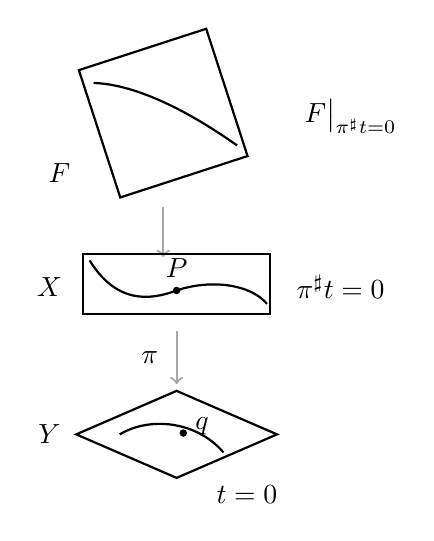
\begin{tikzpicture}[scale=0.85, line width=0.8pt]
  \begin{scope}[rotate around={18:(1.7,4.6)}]
    \draw (0.7,3.6) rectangle (2.7,5.6);
    \draw (0.85,5.35) .. controls (1.4,5.15) and (2.0,4.6) .. (2.6,3.8);
  \end{scope}
  \node at (0.15,3.7) {$\mathscr{F}$};
  \node at (4.5,4.55) {$\mathscr{F}\bigr|_{\pi^{\sharp}t=0}$};
  \draw[gray!70,->] (1.7,3.2) -- (1.7,2.45);
  \draw (0.5,1.6) rectangle (3.3,2.5);
  \draw (0.6,2.4) .. controls (1.0,1.75) and (1.5,1.8) .. (1.9,1.95)
        .. controls (2.4,2.12) and (3.0,2.05) .. (3.25,1.75);
  \fill (1.9,1.95) circle (1.6pt);
  \node at (1.9,2.28) {$P$};
  \node at (0.0,2.0) {$\mathscr{X}$};
  \node at (4.35,2.0) {$\pi^{\sharp}t=0$};
  \draw[gray!70,->] (1.9,1.35) -- (1.9,0.55);
  \node at (1.5,0.95) {$\pi$};
  \draw (1.9,0.45) -- (3.4,-0.2) -- (1.9,-0.85) -- (0.4,-0.2) -- cycle;
  \draw (1.05,-0.2) .. controls (1.5,0.07) and (2.2,0.0) .. (2.6,-0.47);
  \fill (2.0,-0.18) circle (1.6pt);
  \node at (2.28,-0.08) {$q$};
  \node at (0.0,-0.2) {$\mathscr{Y}$};
  \node at (2.95,-1.1) {$t=0$};
\end{tikzpicture}
\caption{平坦性在靶上的（充分必要的）\trSlicing{}判别法，\mbox{定理~24.6.6}。（依原书手绘图重绘。）}\label{fig:slicing-target-criterion}
\end{figure}

（关于其他性质的\trSlicing{}判别法，见\mbox{练习~13.2.C}、\mbox{定理~24.6.9} 与\mbox{定理~26.2.3}。）

为证此定理，我们先证一条引理，它还将用于证明\mbox{定理~24.6.14}。（注意：它对局部环或有限生成不作任何假设。）

\textbf{24.6.7. \trhLemma。}\ ——\ \emph{设 $I\subset B$ 是一个\trIdeal，$M$ 是一个 $B$-\trModule。又设（i）$\mathrm{Tor}^B_1(B/I,M)=0$，且（ii）$M/IM$ 在 $B/I$ 上平坦。则对每个包含 $I$ 的\trIdeal{} $J$ 都有 $\mathrm{Tor}^B_1(B/J,M)=0$。}

\emph{证明。}\quad 函子 $\otimes_B B/J$ 是函子 $\otimes_B B/I$ 与函子 $\otimes_{B/I}B/J$ 的复合。由\trGrothendieck{}函子复合谱序列（\S23.3.5），存在一个谱序列，其 $\Eto{p,q}{2}$ 项为 $\mathrm{Tor}^{B/I}_p\bigl(B/J,\mathrm{Tor}^B_q(B/I,M)\bigr)$，抵达 $\mathrm{Tor}^B_{p+q}(B/J,M)$。定理的假设保证
\[
\mathrm{Tor}^{B/I}_0\bigl(B/J,\mathrm{Tor}^B_1(B/I,M)\bigr)=0
\]
（由 (i)），以及
\[
\mathrm{Tor}^{B/I}_1\bigl(B/J,\mathrm{Tor}^B_0(B/I,M)\bigr)=\mathrm{Tor}^{B/I}_1(B/J,M/IM)=0
\]
（由 (ii)；这里对 $B/I$ 用了平坦性的理想论判别法，\mbox{定理~24.3.1}）。于是 $\mathrm{Tor}^B_1(B/J,M)=0$，此即所欲证。（不借谱序列这台机器，本证明也可以干脆用手工完成。）\hfill$\square$

\textbf{24.6.8.}\ \emph{平坦性在靶上的\trSlicing{}判别法（\mbox{定理~24.6.6}）的证明。}\quad 于是，在前一条引理中取 $I=(t)$、$J=\mathfrak{n}$，并利用\mbox{练习~24.2.A} 所给的 $\mathrm{Tor}^B_1(B/tB,M)=\ker(M\xrightarrow{\ \times t\ }M)$——由假设它为零——\mbox{定理~24.6.6} 便随之而得。\hfill$\square$

\textbf{24.6.A.（练习）}\quad 用\trSlicing{}判别法给出\mbox{练习~24.3.I}（$\mathbb{P}^4$ 中交于一点的两张平面）的第二个解法。（这只会用到\trSlicing{}判别法的「容易方向」。）

下面是一个类似的平坦性\trSlicing{}判别法，不过是在\emph{源}上的。注意：这个判别法只在一个方向上成立。

\textbf{24.6.9. \trhTheorem（平坦性在源上的\trSlicing{}判别法，见图~\ref{fig:slicing-source-criterion}）。}\ ——\ \emph{设 $(B,\mathfrak{n})\to(A,\mathfrak{m})$ 是\trNoether{}局部环之间的一个局部态射，$M$ 是有限生成的 $A$-\trModule，而 $t\in\mathfrak{m}\subset A$ 在 $M/\mathfrak{n}M$ 上不是\trZerodivisor。若 $M$ 在 $B$ 上平坦，则 $M/tM$ 在 $B$ 上平坦。}

\begin{figure}[htbp]
\centering
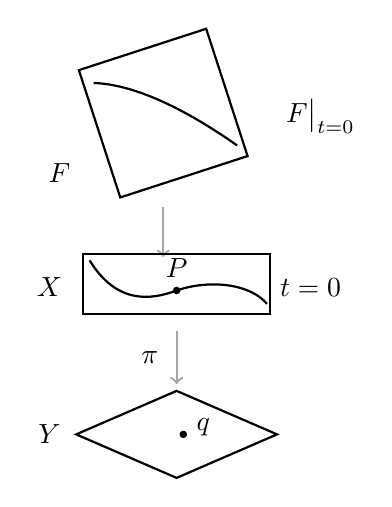
\begin{tikzpicture}[scale=0.85, line width=0.8pt]
  \begin{scope}[rotate around={18:(1.7,4.6)}]
    \draw (0.7,3.6) rectangle (2.7,5.6);
    \draw (0.85,5.35) .. controls (1.4,5.15) and (2.0,4.6) .. (2.6,3.8);
  \end{scope}
  \node at (0.15,3.7) {$\mathscr{F}$};
  \node at (4.05,4.55) {$\mathscr{F}\bigr|_{t=0}$};
  \draw[gray!70,->] (1.7,3.2) -- (1.7,2.45);
  \draw (0.5,1.6) rectangle (3.3,2.5);
  \draw (0.6,2.4) .. controls (1.0,1.75) and (1.5,1.8) .. (1.9,1.95)
        .. controls (2.4,2.12) and (3.0,2.05) .. (3.25,1.75);
  \fill (1.9,1.95) circle (1.6pt);
  \node at (1.9,2.28) {$P$};
  \node at (0.0,2.0) {$\mathscr{X}$};
  \node at (3.9,2.0) {$t=0$};
  \draw[gray!70,->] (1.9,1.35) -- (1.9,0.55);
  \node at (1.5,0.95) {$\pi$};
  \draw (1.9,0.45) -- (3.4,-0.2) -- (1.9,-0.85) -- (0.4,-0.2) -- cycle;
  \fill (2.0,-0.2) circle (1.6pt);
  \node at (2.3,-0.1) {$q$};
  \node at (0.0,-0.2) {$\mathscr{Y}$};
\end{tikzpicture}
\caption{平坦性在源上的（充分的）\trSlicing{}判别法，\mbox{定理~24.6.9}。（依原书手绘图重绘。）}\label{fig:slicing-source-criterion}
\end{figure}

\emph{证明。}\quad 我们有 $A$-\trModule{}（从而也是 $B$-\trModule）的一个\trExactSequence
\[
M \xrightarrow{\ \times t\ } M \longrightarrow M/tM \longrightarrow 0.
\]
把它延拓成 $B$-\trModule{}的一个平坦分解（例如，用自由的 $B$-\trModule{}向左搭出来）：
\[
\tag{24.6.9.1}\label{eq:slicing-source-resolution}
\cdots \longrightarrow M \xrightarrow{\ \times t\ } M \longrightarrow M/tM \longrightarrow 0.
\]
我们可以用任何平坦分解来计算 $\mathrm{Tor}^B_1(M/tM,B/\mathfrak{n})$（\mbox{练习~23.3.D}）。\footnote{译注：原书此处与下文两处均作「$\mathrm{Tor}^B_1(B/tM,B/\mathfrak{n})$」，当为「$\mathrm{Tor}^B_1(M/tM,B/\mathfrak{n})$」之误——\eqref{eq:slicing-source-resolution} 所分解的对象是 $M/tM$，而非「$B/tM$」，径改。——译者注}于是我们使用 \eqref{eq:slicing-source-resolution}。把 $\otimes_B B/\mathfrak{n}$ 作用到 \eqref{eq:slicing-source-resolution} 上，并截去最右一项，便得到这样的\trComplexN，其上同调将给出 $\mathrm{Tor}^B_1(M/tM,B/\mathfrak{n})$：
\[
\cdots \longrightarrow M/\mathfrak{n} \xrightarrow{\ \times t\ } M/\mathfrak{n} \longrightarrow 0.
\]
但由假设，$\times t\colon M/\mathfrak{n}\to M/\mathfrak{n}$ 的\trKernel{}为零，故第一步处的上同调为零，从而我们有 $\mathrm{Tor}^B_1(M/tM,B/\mathfrak{n})=0$。再由平坦性的局部判别法（\mbox{定理~24.6.1}），$M/tM$\footnote{译注：原书此处作「$M/tN$」，当为「$M/tM$」之误，径改。——译者注}在 $B$ 上平坦，此即所欲证。\hfill$\square$

\textbf{24.6.10.}\ \extrahard\ \emph{相对有效\trCartier{}除子。}\quad \mbox{定理~24.6.9} 有一个直接的几何解读：「设 $\pi\colon X\to Y$ 是\trNoether{}概形之间的一个\trMorphism，$\mathscr{F}$ 是 $X$ 上的一个\trCoherentSheaf，而 $Z\hookrightarrow X$ 是一个局部主子概形……」。在 $\mathscr{F}=\OO_X$ 的特殊情形，这就引出了\textbf{相对有效\trCartier{}除子}（relative effective Cartier divisor）的概念：$X$ 的一个局部主子概形，它在 $\pi$ 的一切纤维上都是\trEffectiveCartierDivisor。\mbox{定理~24.6.9} 蕴含：若 $\pi$ 平坦，则任何相对有效\trCartier{}除子也是平坦的。（一个重要应用见\mbox{练习~25.3.H}。）

\textbf{24.6.11. 在域上，正则嵌入是仿射空间中诸坐标轴的局部平坦覆盖。}

\textbf{24.6.B.（有用的练习）}\quad 设 $(A,\mathfrak{m})$ 是一个\trNoether{}局部环，其中 $A$ 包含一个域 $k$（即 $A$ 是一个 $k$-\trAlgebra）。设 $f_1,\dots,f_n\in\mathfrak{m}$。这 $n$ 个 $\Spec A$ 上的函数确定一个\trMorphism{} $\pi\colon\Spec A\to\mathbb{A}^n_k$。证明：$\pi$ 平坦，当且仅当 $f_1,\dots,f_n$ 构成一个\trRegularSequence。更一般地，若 $M$ 是一个有限生成的 $A$-\trModule，证明：$M$ 在 $\mathbb{A}^n_k$ 上平坦，当且仅当 $f_1,\dots,f_n$ 构成一个 $M$-\trRegularSequence。提示：平坦性在靶上的\trSlicing{}判别法，\mbox{定理~24.6.6}。

\mbox{练习~24.6.B} 使许多高深的事实出人意料地变得容易（只要我们是在域 $k$ 上工作）。

\textbf{24.6.C.（练习）}\quad 用\mbox{练习~24.6.B} 给\mbox{定理~9.5.6} 一个直接的证明：$\mathfrak{m}$ 中的 $M$-\trRegularSequence{}在任意重排之下仍是正则的，只要 $A$ 是某个 $k$-\trAlgebra。（「\trMixedCharacteristic」的情形未被覆盖。）我们原来的证明明显更难（尽管更一般）。

\textbf{24.6.D.（练习）}\quad 用\mbox{练习~24.6.B} 重证：\trNoether{} $k$-\trScheme{}中余维数为 $r$ 的\trRegularEmbedding，其（余）正规层是秩 $r$ 的\trLocallyFreeSheaf（\mbox{命题~21.2.16}(b) 的 $k$-\trScheme{}版本）。

\textbf{24.6.E.（练习，参看\mbox{练习~24.1.O}）}\quad 用\mbox{练习~24.6.B} 重证：若 $\mathscr{I}$ 是\trNoether{} $k$-\trScheme{}中余维数为 $r$ 的\trRegularEmbedding{}的理想层，则自然映射 $\Sym^n(\mathscr{I}/\mathscr{I}^2)\to\mathscr{I}^n/\mathscr{I}^{n+1}$ 是\trIsomorphism（\mbox{推论~22.3.9} 的 $k$-\trScheme{}版本）。

\textbf{24.6.F.}\ \extrahard\ \textbf{（练习）}\quad 本练习要用到\mbox{练习~24.4.A}。设 $(A,\mathfrak{m})$ 是一个含域 $k$ 的\trNoether{}局部环，$f_1,\dots,f_r$ 是 $\mathfrak{m}$ 中的一个\trRegularSequence，而 $s$ 把 $E=A^{\oplus r}$ 的第 $i$ 个基元送到 $f_i$。用\mbox{练习~24.6.B} 证明：Koszul 复形 $K_\bullet(s)$（\S24.4.1）正合，唯独在最后一项例外，那里的上同调是 $A/(f_1,\dots,f_r)$。（更一般的陈述见\mbox{练习~24.4.C}。）

\textbf{24.6.12.}\ \extrahard\ \textbf{\trFiber{}平坦性。}\quad 我们以一条可能非常有用的平坦性判别法来收尾，但全书余下的部分并不需要它。它适用于如下由局部\trNoether{}概形组成的交换图，并且其中 $\mathscr{F}$ 是 $X$ 上的一个\trCoherentSheaf：
\[
\begin{tikzcd}[row sep=2.2em, column sep=3.6em]
X \ar[rr, "\pi"] \ar[dr, "\tau"'] & & Y \ar[dl, "\rho"] \\
& Z &
\end{tikzcd}
\]
对每一点 $r\in Z$，令 $\pi_r\colon X_r\to Y_r$ 为 $\pi$ 的基变换。

\textbf{24.6.13. \trFiber{}平坦性定理，版本一。}\ ——\ \emph{设 $\mathscr{F}$ 在 $Z$ 上平坦，且对每一点 $r\in Z$，$\mathscr{F}|_{X_r}$ 在 $Y_r$ 上平坦。则 $\mathscr{F}$ 在 $Y$ 上平坦。}

\textbf{24.6.G.（练习）}\quad 证明：要证\mbox{定理~24.6.13}，只须证明下面这条。

\textbf{24.6.14. \trFiber{}平坦性定理，交换代数版本一。}\ ——\ \emph{设}
\begin{equation*}
\tag{24.6.14.1}\label{eq:fibral-flatness-diagram}
\begin{tikzcd}[row sep=2.4em, column sep=3.4em]
(A,\mathfrak{m}) & & (B,\mathfrak{n}) \ar[ll] \\
& (R,\mathfrak{r}) \ar[ul] \ar[ur]
\end{tikzcd}
\end{equation*}
\emph{是\trNoether{}局部环的一个交换图（照例把极大理想送到极大理想），而 $M$ 是一个有限生成的 $A$-\trModule。设 $M$ 在 $R$ 上平坦，且 $M/\mathfrak{r}M$ 在 $B/\mathfrak{r}B$ 上平坦。则 $M$ 在 $B$ 上平坦。}

\emph{证明。}\quad 我们将使用\mbox{引理~24.6.7}。我们希望证明 $\mathrm{Tor}^B_1(M,B/\mathfrak{n})=0$（以便援引平坦性的局部判别法，\mbox{定理~24.6.1}）；又已知 $M/\mathfrak{r}M$ 在 $B/\mathfrak{r}B$ 上平坦，因此我们希望对模 $M$、环 $B$、理想 $J=\mathfrak{n}$ 与 $I=\mathfrak{r}B$ 应用\mbox{引理~24.6.7}。\mbox{引理~24.6.7} 尚待检验的假设只剩：$\mathrm{Tor}^B_1(M,B/\mathfrak{r}B)=0$。

把右正合函子 $\cdot\otimes_B M$ 作用到 $B$-\trModule{}的满态射 $\mathfrak{r}\otimes_R B\twoheadrightarrow\mathfrak{r}B$ 上，便得到一个满态射
\[
\alpha\colon \mathfrak{r}\otimes_R M=\mathfrak{r}\otimes_R B\otimes_B M \twoheadrightarrow (\mathfrak{r}B)\otimes_B M.
\]
考虑 $B$-\trModule{}映射的复合 $\gamma$：
\[
\mathfrak{r}\otimes_R M \xrightarrow{\ \alpha\ } (\mathfrak{r}B)\otimes_B M \xrightarrow{\ \beta\ } M.
\]
现在 $\alpha$ 是满射，而复合 $\beta\circ\alpha$ 是\trInjectiveMap（把 $\cdot\otimes_R M$ 作用到 $0\to\mathfrak{r}\to R$ 上，并利用 $M$ 在 $R$ 上平坦）。于是 $\alpha$ 必为\trInjectiveMap，从而是\trIsomorphism，进而 $\beta$ 必为\trInjectiveMap。

接下来，把 $M\otimes_B\cdot$ 作用到短正合列
\[
0 \longrightarrow \mathfrak{r}B \longrightarrow B \longrightarrow B/\mathfrak{r}B \longrightarrow 0
\]
上。由于 $B$ 在 $B$ 上平坦，$\mathrm{Tor}^B_1(M,B)=0$，于是我们有正合列
\[
\begin{tikzcd}[row sep=2em, column sep=1.9em]
0=\mathrm{Tor}^B_1(M,B) \ar[r] & \mathrm{Tor}^B_1(M,B/\mathfrak{r}B) \ar[dl] & \\
M\otimes_B\mathfrak{r}B \ar[r, "\beta"] & M\otimes_B B \ar[r] & M\otimes_B B/\mathfrak{r}B \ar[r] & 0.
\end{tikzcd}
\]
由 $\beta$ 的\trInjectiveMap{}性得 $\mathrm{Tor}^B_1(M,B/\mathfrak{r}B)=0$，此即所欲证。\footnote{译注：原书此处作「$\mathrm{Tor}^R_1(M,B/\mathfrak{r}B)$」，其上标当为 $B$（所证者即 $\mathrm{Tor}^B_1$ 的消失），径改。——译者注}\hfill$\square$

\mbox{定理~24.6.14} 可以推广为下面这条（它同样可以引出与\mbox{定理~24.6.13} 类似的几何陈述）。

\textbf{24.6.15. \trFiber{}平坦性定理，交换代数版本二。}\ ——\ \emph{设 \eqref{eq:fibral-flatness-diagram} 是\trNoether{}局部环的一个交换图，而 $M$ 是一个\textbf{非零}的有限生成 $A$-\trModule。则 (a) 成立当且仅当 (b) 成立。}
\begin{itemize}
\item[(a)]\emph{(i) $M$ 在 $R$ 上平坦，且 (ii) $M/\mathfrak{r}M$ 在 $B/\mathfrak{r}B$ 上平坦。}
\item[(b)]\emph{(i) $M$ 在 $B$ 上平坦，且 (ii) $B$ 在 $R$ 上平坦。}
\end{itemize}

\textbf{24.6.H.（容易练习）}\quad 证明：(b) 蕴含 (a)。

\emph{证明。}\quad 结论的大部分已在\mbox{定理~24.6.14} 与\mbox{练习~24.6.H} 中证得。剩下的只须证明：(a)(i)、(a)(ii) 与 (b)(i) 蕴含 (b)(ii)。

\textbf{24.6.I.（练习）}\quad 证明：(a)(i)、(a)(ii) 与 (b)(i) 蕴含 $M$ 在 $B$ 上忠实平坦。

现在我们直接证明 $B$ 在 $R$ 上平坦。设 $N_\bullet$ 是 $R$-\trModule{}的一个\trExactSequence。我们希望证明 $B\otimes_R N_\bullet$ 正合。而由 (a)(i)，$M\otimes_R N_\bullet$ 正合，并且 $M\otimes_R N_\bullet=M\otimes_B(B\otimes_R N_\bullet)$ 正合。由于 $M$ 在 $B$ 上忠实平坦，便知 $B\otimes_R N_\bullet$ 正合，此即所欲证。\hfill$\square$




\section{平坦性蕴含欧拉示性数恒常}

我们来实现 \S24.0.1 中许诺过的\trFlatness{}的一个重要推论。将会看到，这一结果为许多我们在还不知道平坦性时就该问起的问题给出答案与实例。

\textbf{24.7.1. 重要定理（欧拉示性数在平坦\trFamily{}中恒常）。}\ ——\ \emph{设 $\pi\colon X\to Y$ 是局部\trNoether{}\trScheme{}之间的一个\trProjective{}\trMorphism，$\mathscr{F}$ 是 $X$ 上的一个\trCoherentSheaf，在 $Y$ 上\trFlat。则 $\chi(X_q,\mathscr{F}|_{X_q})=\sum_{i\ge 0}(-1)^i h^i(X_q,\mathscr{F}|_{X_q})$ 是 $q\in Y$ 的\trLocallyConstant{}函数（其中 $X_q=\pi^{-1}(q)$）。}

这是「\trCohomology{}在平坦\trFamily{}中表现良好」的第一个征兆。（我们很快将看到第二个征兆：\mbox{\trSemicontinuity{}定理~25.1.1}。\mbox{定理~24.7.1} 的另一个证明——它把结果推广到\trProper{}情形——将在 \S25.2.5 中给出。）诸\trNoether{}假设的用途，在于保证 $\pi_\ast\mathscr{F}(m)$ 是\trCoherentSheaf。

\mbox{定理~24.7.1} 给出了平坦性的一个必要条件。它的逆命题（给出充分条件）见\mbox{练习~24.7.C}。

\emph{证明。}\quad 我们先作三个快速的化归。（i）这个问题在靶 $Y$ 上局部，故可化归到 $Y$ 仿射的情形，比如说 $Y=\Spec B$，于是 $\pi$ 可通过某个\trClosedEmbedding{} $X\hookrightarrow\mathbb{P}^n_B$（$n$ 为某个数）分解。（ii）把 $\mathscr{F}$ 视为 $\mathbb{P}^n_B$ 上的\trSheaf，便可化归到 $X=\mathbb{P}^n_B$ 的情形。（iii）可化归为证明：对 $m\gg 0$，$h^0(X_q,\mathscr{F}(m)|_{X_q})$ 是 $q\in Y$ 的\trLocallyConstant{}函数，并且当 $i>0$ 时 $h^i(X_q,\mathscr{F}(m)|_{X_q})=0$。（由\trSerre{}消失，当 $i>0$ 且 $m\gg 0$ 时确有 $h^i(X_q,\mathscr{F}(m)|_{X_q})=0$，但先验地每个 $q$ 可各有不同的 $m$，而我们需要 $m$ 不依赖于 $q$。）

取 $m\gg 0$ 并用 $\OO(m)$ 扭转，使得 $\mathscr{F}$ 的高阶\trCohomology{} $\mathrm{H}^{i>0}(X,\mathscr{F}(m))$ 全部消失（由\trSerre{}消失，\mbox{定理~18.1.3}~(ii)）。现在考虑 $\mathscr{F}(m)$ 的\trCech\trComplexN{} $\mathscr{C}^{\bullet}$。注意：由于 $\mathscr{F}$ \trFlat，\trCech\trComplexN{} $\mathscr{C}^{\bullet}$ 的所有项都是平坦的。（你看出缘由了吗？）既然所有高阶\trCohomology{}群（\trHigherPushforward）都消失，$\mathscr{C}^{\bullet}$ 除首项外正合，而首项处的\trCohomology{}是 $\Gamma(\pi_\ast\mathscr{F}(m))$。我们把\trModule{} $\Gamma(\pi_\ast\mathscr{F}(m))$ 添到复形的最前端，它便再次正合：
\[
\tag{24.7.1.1}\label{eq:flat-cech-resolution}
0 \longrightarrow \Gamma(\pi_\ast\mathscr{F}(m)) \longrightarrow \mathscr{C}^1 \longrightarrow \mathscr{C}^2 \longrightarrow \cdots \longrightarrow \mathscr{C}^{n+1} \longrightarrow 0.
\]
（这种把一个\trModule{}「接上去」的把戏我们以前也干过，例如 \eqref{eq:extended-cech-complex}。）于是，由练习~24.2.G，我们有一条除首项外诸项皆平坦的正合列，故首项也是平坦的。于是 $\pi_\ast\mathscr{F}(m)$ 是 $Y$ 上一个平坦的\trCoherentSheaf，从而是\trLocallyFree{}的（\mbox{推论~24.3.7}），从而具有\trLocallyConstant{}的\trRank。

设 $q\in Y$。我们想证明\trHilbert{}函数 $h_{\mathscr{F}|_{X_q}}(m)$ 是 $q$ 的\trLocallyConstant{}函数。为计算 $h_{\mathscr{F}|_{X_q}}(m)$，我们把\trCech{}分解与 $\kappa(q)$ 作张量，再取\trCohomology。\trCech{}分解加上前端所接的 $\Gamma(\pi_\ast\mathscr{F}(m))$——即 \eqref{eq:flat-cech-resolution}——是平坦\trModule{}的正合列，因而与 $\kappa(q)$ 作张量后仍保持正合（\mbox{练习~24.2.F}）。于是
\[
\Gamma(\pi_\ast\mathscr{F}(m))\otimes\kappa(q)\cong\Gamma(\pi_\ast\mathscr{F}(m)|_q),
\]
所以\trHilbert{}函数 $h_{\mathscr{F}|_{X_q}}(m)$ 就是某个\trLocallyFreeSheaf{}在 $q$ 处的\trRank，而这乃是 $q\in Y$ 的\trLocallyConstant{}函数。\hfill$\square$

现在我们来给出\mbox{定理~24.7.1} 的几个有用得离谱的推论。

\textbf{24.7.2. \trhCorollary。}\ ——\ \emph{采用与\mbox{定理~24.7.1} 相同的假设与记号。则 $\mathscr{F}|_{X_q}$ 的\trHilbertPolynomial{}作为 $q\in Y$ 的函数是\trLocallyConstant{}的。}

\textbf{24.7.A.（关键练习）}\quad 设 $X\to Y$ 是\trProjective{}\trFlat{}\trMorphism，其中 $Y$ \trConnected。证明：$q\in Y$ 的下列函数都是常数：（a）\trFiber{}的\trDegree；（b）\trFiber{}的\trDimension；（c）\trFiber{}的\trArithmeticGenus。

\textbf{24.7.B.（练习）}\quad 用 \S24.3.9 与\mbox{练习~24.7.A}(a)，给出\mbox{练习~16.3.D}(a)（「从无\trEmbeddedPoint{}的\trCurve{}到\trIrreducible\trRegular\trCurve{}的\trFinite\trMorphism{}具有常值的\trDegree」）的另一个解法。

\textbf{24.7.C.（不重要练习（\mbox{定理~24.7.1} 的逆命题））}\quad （这个练习我们不会用在任何地方。）
（a）设 $A$ 是\trRing，$S_\bullet$ 是一个在 $A$ 上平坦的有限生成 $A$-\trAlgebra。证明 $\Proj S_\bullet$ 在 $A$ 上\trFlat。
（b）设 $\pi\colon X\to Y$ 是局部\trNoether{}\trScheme{}之间的一个\trProjective{}\trMorphism（一如既往，这包括 $X$ 上一个\trInvertibleSheaf{} $\OO_X(1)$ 的数据），使得对某个 $m_0$ 及一切 $m\ge m_0$，$\pi_\ast\OO_X(m)$ 都是\trLocallyFree{}的。证明 $\pi$ \trFlat。提示：把 $X$ 描述为
\[
\Proj\left(\OO_Y\oplus\Bigl(\bigoplus_{m\ge m_0}\pi_\ast\OO_X(m)\Bigr)\right).
\]
（c）更一般地，设 $\pi\colon X\to Y$ 是局部\trNoether{}\trScheme{}之间的一个\trProjective{}\trMorphism，$\mathscr{F}$ 是 $X$ 上的一个\trCoherentSheaf，使得对某个 $m_0$ 及一切 $m\ge m_0$，$\pi_\ast\mathscr{F}(m)$ 都是\trLocallyFree{}的。证明 $\mathscr{F}$ 在 $Y$ 上\trFlat。
（d）设 $\pi\colon X\to Y$ 是局部\trNoether{}\trScheme{}之间的一个\trProjective{}\trMorphism，$\mathscr{F}$ 是 $X$ 上的一个\trCoherentSheaf，使得 $\mathscr{F}|_{X_q}$ 的\trHilbertPolynomial{}是 $q\in Y$ 的\trLocallyConstant{}函数。若 $Y$ \trReduced，证明 $\mathscr{F}$ 必在 $Y$ 上\trFlat。（提示：\mbox{练习~14.3.K} 表明，在特别好的情形中，常\trRank{}蕴含\trLocallyFree{}性。）

\mbox{推论~24.7.2} 的另一个推论，则惊人地有用。

\textbf{24.7.3. \trhCorollary。}\ ——\ \emph{平坦\trProjective{}\trCurve{}\trFamily{} $X$ 上的\trInvertibleSheaf{} $\mathscr{L}$，在诸\trFiber{}上具有\trLocallyConstant{}的\trDegree。}

（回想：\trProjective{}\trCurve{}上\trLineBundle{}之\trDegree{}的定义，不需要对\trCurve{}附加诸如\trRegularity{}之类的假设；见 \eqref{eq:degree-coherent-sheaf}。）

\emph{证明。}\quad 平坦\trCurve{}\trFamily{}上的\trInvertibleSheaf{} $\mathscr{L}$ 总是平坦的（因为局部地它同构于\trStructureSheaf）。于是 $\chi(X_q,\mathscr{L}_q)$ 是 $q$ 的常值函数。按 \eqref{eq:degree-coherent-sheaf} 给出的\trDegree{}定义，$\deg(X_q,\mathscr{L}_q)=\chi(X_q,\mathscr{L}_q)-\chi(X_q,\OO_{X_q})$。结论便由两者皆\trLocallyConstant（\mbox{定理~24.7.1}）得到。\hfill$\square$

下面的练习是\mbox{推论~24.7.3} 的一个实质性的推广。

\textbf{24.7.D.}\ \hard\ \textbf{（供已读过加星的第 20 章者的练习：\trIntersectionNumber{}在平坦\trFamily{}中\trLocallyConstant）}\quad 设 $\pi\colon X\to Y$ 是到一个\trConnected\trScheme{}的\trFlat\trProjective{}\trMorphism；$\mathscr{L}_1,\dots,\mathscr{L}_n$ 是 $X$ 上的诸\trLineBundle；$\mathscr{F}$ 是 $X$ 上的一个\trCoherentSheaf，在 $Y$ 上\trFlat，且 $\mathscr{F}$ 限制到 $\pi$ 的任一\trFiber{}上时\trSupport{}的\trDimension{}至多为 $n$。设 $q$ 是 $Y$ 的任一点，定义（临时记号）$(\mathscr{L}_1\cdot\mathscr{L}_2\cdots\mathscr{L}_n\cdot\mathscr{F})_q$ 为诸 $\mathscr{L}_1,\dots,\mathscr{L}_n$ 与 $\mathscr{F}|_{X_q}$ 在\trFiber{} $X_q$ 上的\trIntersection（\mbox{定义~20.1.1}）。证明 $(\mathscr{L}_1\cdot\mathscr{L}_2\cdots\mathscr{L}_n\cdot\mathscr{F})_q$ 不依赖于 $q$。（利用 \S25.2.5，可把\trProjective{}假设放宽为\trProperness。）

\mbox{推论~24.7.3} 引出如下的讨论。

\textbf{24.7.4. \trhDefinition。}\quad 设 $\mathscr{L}_1$ 与 $\mathscr{L}_2$ 是 $k$-\trVariety{} $X$ 上的两个\trLineBundle。若存在一个\trConnected（但不必\trIrreducible）的 $k$-\trVariety{} $Y$，其上两个 $k$-\trValuedPoint{} $q_1$ 与 $q_2$，以及 $X\times Y$ 上的一个\trLineBundle{} $\mathscr{L}$，使得 $\mathscr{L}$ 限制到 $q_1$、$q_2$ 之上的\trFiber{}分别同构于 $\mathscr{L}_1$ 与 $\mathscr{L}_2$，我们就说 $\mathscr{L}_1$ 与 $\mathscr{L}_2$ \textbf{代数等价}（algebraically equivalent）。

\textbf{24.7.E.}\ \hard\ \textbf{（练习）}\quad 证明「代数等价」的确是一个\trEquivalenceRelation。证明与 $\OO$ 代数等价的诸\trLineBundle{}构成 $\mathrm{Pic}\,X$ 的一个\trSubgroup。这个子群记作 $\mathrm{Pic}^0\,X$。（你将用到「沿同构的\trClosedSubscheme{}把两个\trScheme{}粘合起来」这一概念，\S15.2.12。）\trhWarning{}：尽管它与\trCurve{}上次数 $0$ 的\trLineBundle（\mbox{定义~18.4.2}）的记号不幸完全相同，但这并不是同一个概念。

\textbf{24.7.5.}\ \textbf{N\'eron--Severi 群} $\mathrm{Pic}\,X/\mathrm{Pic}^0\,X$ 是线丛群 $\mathrm{Pic}\,X$ 模代数等价所得的商群。（这一定义曾于 \S18.4.12 许诺。）由\mbox{推论~24.7.3}，代数等价蕴含数值等价（\S18.4.12）：$\mathrm{Pic}^0\,X\subset\mathrm{Pic}^{\tau}\,X$。（旁注：\trProper{} $k$-\trScheme{} $X$ 上的一个\trLineBundle{} $\mathscr{L}$ 是\trNumericallyTrivial{}的，当且仅当存在整数 $m\ne 0$ 使 $\mathscr{L}^{\otimes m}$ 代数平凡。于是 $\mathrm{Pic}^{\tau}\,X/\mathrm{Pic}^0\,X$ 是\trTorsion{}群。其证明见 [SGA6, XIII, Thm.~4.6]；\trProjective{}的情形见 [Laz, Cor.~1.4.38]。）

\textbf{24.7.6.}\ \hard\ \textbf{广中平祐的一个真非\trProjective{}\trSmooth{}三维体之例。}\quad 在 \S15.2.11 中，我们曾造出一个真非\trProjective{}的\trVariety，但它是\trSingular{}的。现在可以利用\mbox{推论~24.7.3} 给出一个\emph{\trSmooth}的例子，它归功于\trHironaka。它在某种意义上是「$\mathbb{P}^3$ 的局部\trBlowup」。\footnote{译注：原书此处作「It is in in some sense」，衍一 in，当为「It is in some sense」之误，径改。——译者注}

在 $\mathbb{P}^3_k$ 内取定两条\trConic{} $C_1$ 与 $C_2$，它们相交于两个（$k$-值）点 $p_1$ 与 $p_2$。我们如下构造一个\trProper{}映射 $\pi\colon X\to\mathbb{P}^3_k$。对 $i=1,2$，令 $U_i=\mathbb{P}^3\setminus\{p_i\}$。对这两个 $i$，考虑\trProjective{}\trMorphism{} $\pi_i\colon X_i\to U_i$：先沿 $C_i$ 胀开，再胀开 $C_{3-i}$ 的\trProperTransform。两个 $\pi_i$ 在 $\mathbb{P}^3\setminus\{p_1,p_2\}$ 之上粘合，给出一个\trMorphism{} $\pi\colon X\to\mathbb{P}^3$。（在 $p_1$ 与 $p_2$ 之外，$C_1$ 与 $C_2$ 不相交，所以先胀开其中一条再胀开另一条，与胀开两者的并是一样的。）

\begin{figure}[htbp]
\centering
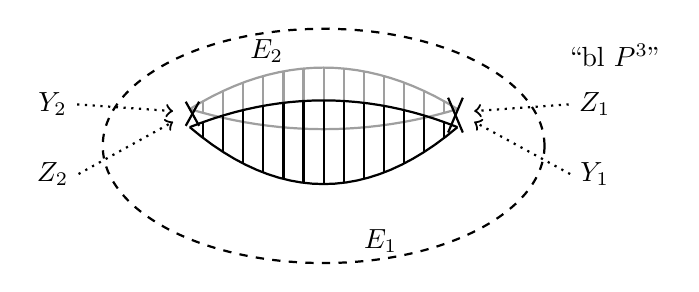
\begin{tikzpicture}[scale=0.85, line width=0.8pt]
  \draw[dashed] (0,0) ellipse (3.3 and 1.75);
  \begin{scope}[gray!75]
    \draw plot[domain=-2.0:2.0] (\x,{0.55+0.62*(1-\x*\x/4)});
    \draw plot[domain=-2.0:2.0] (\x,{0.55-0.30*(1-\x*\x/4)});
    \foreach \x in {-1.8,-1.5,...,1.9}
      \draw (\x,{0.55-0.30*(1-\x*\x/4)}) -- (\x,{0.55+0.62*(1-\x*\x/4)});
  \end{scope}
  \draw plot[domain=-2.0:2.0] (\x,{0.28+0.40*(1-\x*\x/4)});
  \draw plot[domain=-2.0:2.0] (\x,{0.28-0.85*(1-\x*\x/4)});
  \foreach \x in {-1.8,-1.5,...,1.9}
    \draw (\x,{0.28-0.85*(1-\x*\x/4)}) -- (\x,{0.28+0.40*(1-\x*\x/4)});
  \draw (-2.06,0.66) -- (-1.86,0.30);
  \draw (-2.06,0.30) -- (-1.86,0.66);
  \draw (1.86,0.72) -- (2.08,0.20);
  \draw (1.86,0.20) -- (2.08,0.72);
  \node at (-0.85,1.42) {$E_2$};
  \node at (0.85,-1.42) {$E_1$};
  \node (Ytwo) at (-4.05,0.62) {$Y_2$};
  \node (Ztwo) at (-4.05,-0.42) {$Z_2$};
  \node (Zone) at (4.05,0.62) {$Z_1$};
  \node (Yone) at (4.05,-0.42) {$Y_1$};
  \draw[dotted,->] (Ytwo.east) -- (-2.25,0.52);
  \draw[dotted,->] (Ztwo.east) -- (-2.25,0.36);
  \draw[dotted,->] (Zone.west) -- (2.25,0.52);
  \draw[dotted,->] (Yone.west) -- (2.25,0.36);
  \node at (4.35,1.35) {``bl~$\mathbb{P}^3$''};
\end{tikzpicture}
\caption{广中平祐的一个真非\trProjective{}\trSmooth{}三维体之例。（依原书手绘图重绘。）}\label{fig:hironaka-example}
\end{figure}

注意 $\pi$ 是\trProper{}的：它在 $U_1$ 与 $U_2$ 上\trProper，而\trProperness{}这一概念在靶上是局部的（\mbox{命题~11.4.4}(b)）。由于 $\mathbb{P}^3_k$ 是\trProper{}的（在 $k$ 上，\mbox{定理~8.4.10}），而\trProper{}\trMorphism{}的复合仍\trProper（\mbox{命题~11.4.4}(c)），所以 $X$ 是\trProper{}的。

\textbf{24.7.F.（练习）}\quad 证明 $X$ \trSmooth。（提示：\mbox{定理~22.3.10}。）令 $E_i$ 为 $C_i\setminus\{p_1,p_2\}$ 的原像。证明 $\pi|_{E_i}\colon E_i\to C_i\setminus\{p_1,p_2\}$ 是一个 $\mathbb{P}^1$-丛（并且\trFlat）。

\textbf{24.7.G.（练习）}\quad 设 $\overline{E}_i$ 为 $E_i$ 在 $X$ 中的\trClosure。证明 $\overline{E}_i\to C_i$ 是\trFlat{}的。（提示：\mbox{练习~24.3.J}。）

\textbf{24.7.H.（练习）}\quad 证明 $\pi^{-1}(p_i)$ 是两个 $\mathbb{P}^1$ 的并，比如说 $Y_i$ 与 $Z_i$，它们相交于一点，且满足 $Y_i,Y_{3-i},Z_{3-i}\in\overline{E}_i$ 但 $Z_i\notin\overline{E}_i$。

\textbf{24.7.I.（练习）}\quad 按如下思路证明 $X$ 不是\trProjective{}的。假设不然，$\mathscr{L}$ 是 $X$ 上的一个\trVeryAmple{}\trLineBundle，于是 $\mathscr{L}$ 在每条\trCurve{}上都有正的\trDegree（包括诸 $Y_i$ 与 $Z_i$）。利用 $\overline{E}_i\to C_i$ 的\trFlatness{}以及平坦\trFamily{}中\trDegree{}的恒常性（\mbox{练习~24.7.D}），证明 $\deg_{Y_i}\mathscr{L}=\deg_{Y_{3-i}}\mathscr{L}+\deg_{Z_{3-i}}\mathscr{L}$。导出矛盾。（这个论证会让你想起 \S15.2.11 的论证。）

\textbf{24.7.7. 「\trProjective{}\trMorphism」这一概念在靶上不局部。}\quad 注意 $\pi\colon X\to\mathbb{P}^3$ 不是\trProjective{}的，否则 $X$ 就会是\trProjective{}的（因为当最终靶为\trQuasicompact{}时，\trProjective{}\trMorphism{}的复合仍\trProjective，\mbox{练习~17.3.I}）。但在每个 $p_i$ 之外，$\pi$ 都是\trProjective{}的（因为它是诸\trBlowup{}的复合——\trBlowup{}按构造是\trProjective{}的——而最终靶\trQuasicompact，故\mbox{练习~17.3.I} 适用）。于是，「\trProjective{}\trMorphism」这一概念在靶上不局部。（利用 \S15.2.11 可以构造一个更简单但不\trSmooth{}的例子。）


\section{光滑与平展态射，及平坦性}

我们在前面已经定义过光滑\trMorphism{}与平展\trMorphism{}（\mbox{定义~13.6.2}），但直到现在，我们才真正有能力把它们的含义理解得透彻得多。我们将看到，\trUnramified{}态射这一概念（\S21.7）是它们的天然同伴。

我们的这三个代数几何定义，乍看之下并不明显是浑然一体的三胞胎；但我们将会讨论 [Gr-EGA] 中给出的定义（\S24.8.13），而在那套语境下，这三类态射看上去就非常相似了。（我们在 \S24.8.14 中还会简要提及其他的进路与定义。）

本章将要讨论的三类\trMorphism，是微分几何中下列几类流形之间的映射之类似物（参看 \S13.6.1）：
\begin{itemize}
\item \emph{\trSubmersion}是处处诱导\trTangentSpace{}之满射的映射。它们在\trFibration{}这一观念中很有用。（微分几何中或许更贴切、容许奇点的观念是：「在\trSource{}上局部地一个光滑纤维化」。）
\item \emph{在\trSource{}上局部的同构}（isomorphisms locally on the source，或称\emph{局部同构}，local isomorphisms）是诱导\trTangentSpace{}之同构的映射。
\item \emph{\trImmersion}是诱导\trTangentSpace{}之单射的映射。
\end{itemize}
（回想 \S9.2 中的警告：「浸入」一词在代数几何中常以别的含义使用。）

\begin{figure}[htbp]
\centering
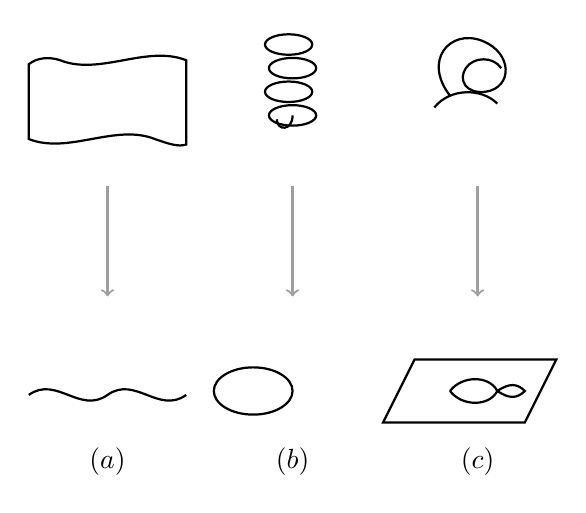
\begin{tikzpicture}[line width=0.8pt]
  \draw (0.0,4.35) .. controls (0.5,4.15) and (1.1,4.55) .. (1.6,4.35)
        .. controls (1.8,4.28) and (1.9,4.25) .. (2.0,4.28)
        -- (2.0,5.35) .. controls (1.5,5.55) and (0.9,5.15) .. (0.4,5.35)
        .. controls (0.25,5.4) and (0.1,5.38) .. (0.0,5.3) -- cycle;
  \draw[gray!75,->] (1.0,3.75) -- (1.0,2.35);
  \draw (0.0,1.1) .. controls (0.35,1.35) and (0.65,0.85) .. (1.0,1.1)
        .. controls (1.35,1.35) and (1.65,0.85) .. (2.0,1.1);
  \node at (1.0,0.25) {$(a)$};
  \draw (3.3,5.55) ellipse (0.30 and 0.13);
  \draw (3.35,5.25) ellipse (0.30 and 0.13);
  \draw (3.30,4.95) ellipse (0.30 and 0.13);
  \draw (3.35,4.65) ellipse (0.30 and 0.13);
  \draw (3.35,4.65) .. controls (3.35,4.45) and (3.15,4.45) .. (3.15,4.6);
  \draw[gray!75,->] (3.35,3.75) -- (3.35,2.35);
  \draw (2.85,1.15) ellipse (0.5 and 0.3);
  \node at (3.35,0.25) {$(b)$};
  \draw (5.35,4.9) .. controls (5.0,5.35) and (5.35,5.75) .. (5.75,5.6)
        .. controls (6.15,5.45) and (6.15,5.0) .. (5.8,4.95)
        .. controls (5.55,4.92) and (5.45,5.1) .. (5.55,5.25)
        .. controls (5.65,5.4) and (5.9,5.4) .. (6.0,5.25);
  \draw (5.15,4.75) .. controls (5.35,5.0) and (5.75,5.0) .. (5.95,4.8);
  \draw[gray!75,->] (5.7,3.75) -- (5.7,2.35);
  \draw (4.9,1.55) -- (6.7,1.55) -- (6.3,0.75) -- (4.5,0.75) -- cycle;
  \draw (5.35,1.15) .. controls (5.5,1.35) and (5.85,1.35) .. (5.95,1.15)
        .. controls (5.85,0.95) and (5.5,0.95) .. (5.35,1.15);
  \draw (5.95,1.15) .. controls (6.1,1.25) and (6.2,1.25) .. (6.3,1.15)
        .. controls (6.2,1.05) and (6.1,1.05) .. (5.95,1.15);
  \node at (5.7,0.25) {$(c)$};
\end{tikzpicture}
\caption{微分几何中诸观念的示意手绘：(a)「在\trSource{}上局部地一个光滑纤维化」的映射，(b) 局部同构，(c) 浸入。（代数几何中分别为：(a) 光滑\trMorphism，(b) 平展\trMorphism，(c) \trUnramified{}态射。）（依原书手绘图重绘。）}\label{fig:diffgeom-smooth-etale-unramified}
\end{figure}

为了更好地理解光滑\trMorphism{}与平展\trMorphism，我们暂时把先前给出的定义抛在脑后，转而考察一些例子：考察一些我们希望成为「局部同构」（或「在\trSource{}上局部地同构」，或「在\trSource{}上局部地一个光滑纤维化」）之类比的东西，看看它们能否帮助我们做出好的定义。

\textbf{24.8.1. 「局部同构」（平展\trMorphism）。}\quad 考虑复数域上抛物线 $x=y^2$ 到 $x$ 轴的投射。（这个例子以这样那样的形式反复出现过，\mbox{练习~13.6.F} 便是一例。）我们有理由希望它在原点之外是（\trSource{}上的）局部同构。我们或许还希望「局部同构」是个开条件型的观念：态射成为局部同构的那些点构成的\trLocus{}应当在\trSource{}上为开。就微分几何中的定义而言，事实的确如此。但这样一来，上述态射就应当在\trGenericPoint{}上是局部同构，而我们在\trGenericPoint{}处得到的是非平凡的\trResidueField{}\trFieldExtension{} $\mathbb{C}(y)/\mathbb{C}(y^2)$，并非\trIsomorphism。于是我们不得不把域的某些有限扩张（的诸 $\Spec$）也看作「\trSource{}上局部的同构」——在这个例子中，甚至是「覆盖空间」。（在\mbox{练习~24.8.D} 中我们将看到，我们想要的恰恰是有限可分扩张；这一点你其实早就能自己证明了。）

还要注意，在这个例子中，不存在非空的\trZariski{}开子集 $U\subset\Spec\mathbb{C}[x]\setminus\{0\}$ 与 $V\subset\Spec\mathbb{C}[x,y]/(x-y^2)\setminus\{(0,0)\}$，使得该映射把 $U$ 同构地送入 $V$（\mbox{练习~13.6.F}），所以这无论如何都不是你先前见过的某种意义下的局部同构。这便引出了\trEtale{}\trTopology{}这一观念——按通常的意义它甚至不是一张\trTopology，而是一个「\trGrothendieck{}\trTopology」（\S6.2.10）。平展\trTopology{}超出了本书的范围。

\textbf{24.8.2. \trSubmersion{}（光滑\trMorphism）。}\quad

\textbf{24.8.3.}\ \emph{纤维是光滑\trVariety。}\quad 作为淹没的代数几何版本的第一近似，我们希望诸\trFiber{}是（剩余域上的）光滑\trVariety。于是头一件需要做的事，就是把「\trVariety」这一观念推广到基上。给这条\trMorphism{}加上局部有限型假设，便可合理地做到这一点。由于某些颇为微妙的原因，我们将要求一个更强的条件：该\trMorphism{}是局部有限表现的。（如果你真想刨根问底，可以在我们的讨论中看到它在何处登场。当然，对诺特读者而言，两种说法没有差别。）

诸\trFiber{}不仅仅是\trVariety；它们还应当是\emph{光滑的}\trVariety（比如说，维数为 $n$）。由域上\trSmoothness{}的情形，或者由我们对光滑\trVariety{}应有的模样的直觉，可以期望\trFiber{}上的微分层是秩 $n$ 的\trLocallyFreeSheaf；更妙的是，可以期望相对微分层是秩 $n$ 的\trLocallyFreeSheaf。

\textbf{24.8.4.}\ \emph{\trFlatness。}\quad 至此，我们对「光滑\trMorphism」的第一近似是「局部有限表现，且纤维是光滑\trVariety」的某个版本。但这还不够。例如，从一个概形 $X$ 到一条\trCurve{} $Y$ 的一个糟糕的映射——它把一个互不相同的正则\trVariety{}送到 $Y$ 的每一点上（$X$ 是这些东西的无穷不交并）——在任何合理的意义下都不应被视为光滑纤维化。另外，我们或许也不想把 $\Spec k[\epsilon]/(\epsilon^2)\to\Spec k$ 视为淹没；比如说，它在\trTangentSpace{}上并非满射，而且更笼统地说，它的图像「看上去不像个纤维化」。

这两个问题都是 $\pi\colon X\to Y$ 未能成为一个良好的「连续」\trFamily{}的表现。凡是在寻找某种模糊的「良好性」观念时，我们都知道，「平坦性」将出现在定义之中。

作为对比，注意「\trUnramified」不含平坦性假设；我们也的确不曾指望它有——因为我们希望原点到 $\mathbb{A}^1$ 的包含（闭嵌入）是\trUnramified{}的。但这样一来，一些古怪的东西也可能是\trUnramified{}的。
\begin{figure}[htbp]
\centering
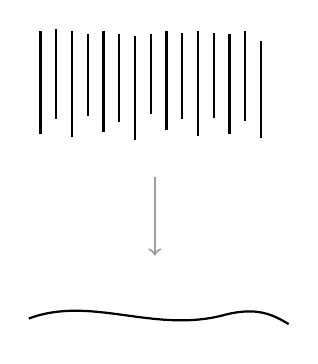
\begin{tikzpicture}[line width=0.8pt]
  \foreach \x/\h/\y in {0.55/1.30/0.00, 0.75/1.15/0.18, 0.95/1.35/-0.05,
    1.15/1.05/0.22, 1.35/1.28/0.02, 1.55/1.12/0.15, 1.75/1.32/-0.08,
    1.95/1.02/0.25, 2.15/1.25/0.05, 2.35/1.10/0.18, 2.55/1.33/-0.03,
    2.75/1.08/0.20, 2.95/1.27/0.00, 3.15/1.14/0.16, 3.35/1.24/-0.06} {
    \draw (\x,\y) -- (\x,\y+\h);
  }
  \draw[gray!75,->] (2.0,-0.55) -- (2.0,-1.55);
  \draw (0.4,-2.35) .. controls (1.2,-2.05) and (2.0,-2.55) .. (2.9,-2.3)
        .. controls (3.3,-2.2) and (3.5,-2.3) .. (3.7,-2.42);
\end{tikzpicture}
\caption{我们不想让这是一个「光滑\trMorphism」。（依原书手绘图重绘。）}\label{fig:not-want-smooth}
\end{figure}

例如，若 $X=\coprod_{z\in\mathbb{C}}\Spec\mathbb{C}$，则把对应于 $z$ 的那个点送到点 $z\in\mathbb{A}^1_{\mathbb{C}}$ 的\trMorphism{} $X\to\mathbb{A}^1_{\mathbb{C}}$ 是\trUnramified{}的。生活就是这样。

\textbf{24.8.5.}\ \emph{期望中的备选定义。}\quad 我们或许可以指望：态射 $\pi\colon X\to Y$ 是\textbf{相对维数 $n$ 光滑}的，当且仅当
（i）$\pi$ 局部有限表现，
（ii）$\pi$ 是相对维数 $n$ 的平坦，且
（iii）$\Omega_{X/Y}$ 是秩 $n$ 的局部自由层。
我们或许同样可以指望：态射 $\pi\colon X\to Y$ 是\textbf{平展}的，当且仅当
（i）$\pi$ 局部有限表现，
（ii）$\pi$ \trFlat，且
（iii）$\Omega_{X/Y}=0$。
我们很快就会证明（分别在\mbox{定理~24.8.8} 与\mbox{练习~24.8.C} 中）：这些期望中的定义与\mbox{定义~13.6.2} 等价。

\textbf{24.8.6. 光滑与平展\trMorphism{}的不同刻画。}\quad 本节的主要结果，是给出光滑\trMorphism{}的若干等价刻画，即\mbox{定理~24.8.8}。我们将先陈述该定理，随后给出它的若干推论，最后才给出证明。作为一条重要的前奏：

\textbf{24.8.7. \trhProposition。}\ ——\ \emph{光滑\trMorphism{}都是\trFlat{}的。}

\emph{证明。}\quad 我们先在诺特情形下证明。设 $\pi\colon X\to Y$ 是局部\trNoether{}概形之间的一个相对维数 $n$ 光滑的\trMorphism。我们希望证明它在一点 $p\in X$ 处平坦。由光滑\trMorphism{}的定义（\S13.6.2），不妨把 $X$ 与 $Y$ 分别换成 $p$ 与 $\pi(p)$ 的仿射邻域，使得 $\pi$ 成为态射
\[
\tag{24.8.7.1}\label{eq:smooth-affine-cover}
\Spec B[x_1,\dots,x_{n+r}]/(f_1,\dots,f_r)\longrightarrow\Spec B,
\]
而 $p$ 是\trJacobianMatrix{}满秩的一点。

\textbf{24.8.A.（练习）}\quad 用源上平坦性的\trSlicing{}判别法（\mbox{定理~24.6.9}）归纳地证明：
\[
\mathbb{A}^{n+r}_{B}\supset V(f_1)\supset V(f_1,f_2)\supset\cdots\supset V(f_1,\dots,f_r)=X
\]

这些概形都在 $p$ 处于 $B$ 上光滑且平坦，从而在诺特情形下证明了\mbox{命题~24.8.7}。（你将需要「光滑 $k$-概形既约」这一事实，\mbox{命题~13.2.13}。）

（诺特读者可以得意洋洋地直接跳到证明的末尾。）我们用一个狡猾的招数来证明一般情形。我们仍把 $\pi$ 局部地写成 \eqref{eq:smooth-affine-cover}。通过重新安排诸 $x$-变量的次序，不妨假设 $f_1,\dots,f_r$ 关于前 $r$ 个变量 $x_1,\dots,x_r$ 的\trJacobianMatrix{}是可逆的。设
\[
f_i(x_1,\dots,x_{n+r})=\sum_{a^i_1,\dots,a^i_{n+r}}b^i_{a^i_1,\dots,a^i_{n+r}}\,x_1^{a^i_1}\cdots x_{n+r}^{a^i_{n+r}},
\]
其中 $b^i_{j,\dots,k}\in B$。（这些都是有限和！）考虑多项式代数 $P=\mathbb{Z}[c^i_{j,\dots,k}]$，其中诸 $c$-变量的指标恰好取诸 $b$-变量的指标中出现过的那些。定义 $g_i\in P[x_1,\dots,x_{n+r}]$ 如下：
\[
g_i(x_1,\dots,x_{n+r})=\sum_{a^i_1,\dots,a^i_{n+r}}c^i_{a^i_1,\dots,a^i_{n+r}}\,x_1^{a^i_1}\cdots x_{n+r}^{a^i_{n+r}}.
\]
设 $J\in P[x_1,\dots,x_{n+r}]$ 是 $g_1,\dots,g_r$ 关于 $x_1,\dots,x_r$ 的\trJacobianMatrix{}的行列式。最后，令 $R:=P_J$。我们有一张\trCartesianDiagram
\[
\begin{tikzcd}[row sep=3.2em, column sep=6.5em]
\Spec B[x_1,\dots,x_{n+r}]/(f_1,\dots,f_r) \ar[r] \ar[d, "\pi"'] & \Spec R[x_1,\dots,x_{n+r}]/(g_1,\dots,g_r) \ar[d, "\alpha"] \\
\Spec B \ar[r] & \Spec R
\end{tikzcd}
\]
它把 $c^i_{j,\dots,k}$ 送到 $b^i_{j,\dots,k}$，并把 $g_i$ 送到 $f_i$。由于 $J$ 在 $R$ 中可逆，$\alpha$ 是相对维数 $n$ 光滑的（基本上就是定义）。由这一结果已证的诺特情形，$\alpha$ 是\trFlat{}的。而平坦性在\trBaseChange{}下保持，故 $\pi$ \trFlat，正如所愿。\hfill$\square$

现在我们来到本节的中心结果。

\textbf{24.8.8. \trhTheorem。}\ ——\ \emph{设 $\pi\colon X\to Y$ 是概形之间的一个\trMorphism。则下列诸条等价。}
（i）\emph{\trMorphism{} $\pi$ 是相对维数 $n$ 光滑的（\mbox{定义~13.6.2}）。}
（ii）\emph{\trMorphism{} $\pi$ 局部有限表现且是相对维数 $n$ 的平坦；并且 $\Omega_\pi$ 是秩 $n$ 的局部自由层（\mbox{期望中的备选定义~24.8.5}）。}
（iii）\emph{\trMorphism{} $\pi$ 局部有限表现且\trFlat，并且诸\trFiber{}是纯维数 $n$ 的光滑 $k$-概形。}
（iv）\emph{\trMorphism{} $\pi$ 局部有限表现且\trFlat，并且诸几何纤维是纯维数 $n$ 的光滑 $k$-概形。}

我们先把这条定理中那些基本上已经证明过的部分解决掉。

\textbf{24.8.B.（练习）}\quad 证明 (i) 蕴涵 (ii) 蕴涵 (iii)，并证明 (iii) 与 (iv) 等价。提示（依次为）：光滑蕴涵平坦，用\mbox{命题~24.8.7}；以微分给出的光滑 $k$-\trVariety{}的定义，见\mbox{重新定义~21.2.28}；\trSmoothness{}与域扩张无关，用\mbox{练习~13.2.H}。

在 \S24.8.11 中完成\mbox{定理~24.8.8} 的证明之前，我们先给出若干道练习与几条假定它成立的结果，以期为这一结果提供动机。

\textbf{24.8.C.（练习）}\quad 证明：态射 $\pi$ 是平展的（\mbox{定义~13.6.2}），当且仅当 $\pi$ 局部有限表现、\trFlat，并且 $\Omega_\pi=0$（\mbox{期望中的备选定义~24.8.5}）。

\textbf{24.8.D.（容易练习）}\quad 设 $\pi\colon X\to Y$ 是一个\trMorphism。证明下列诸条等价。
（a）$\pi$ 平展。
（b）$\pi$ 光滑且\trUnramified。
（c）$\pi$ 局部有限表现、平坦且\trUnramified。
（d）$\pi$ 局部有限表现、平坦，并且对每个 $q\in Y$，$\pi^{-1}(q)$ 都是形如 $\Spec K$ 的概形的不交并，其中 $K$ 是 $\kappa(q)$ 的一个有限可分扩张。
（e）$\pi$ 局部有限表现、平坦，并且对 $Y$ 的每个\emph{\trGeometricPoint}{} $\overline{q}$，$\pi^{-1}(\overline{q})$ 都是若干份 $\overline{q}$ 拷贝的不交并。

\textbf{24.8.E.（重要练习）}\quad 设 $\pi\colon X\to Y$ 平展。证明：局部环维数为 $n$ 的正则点 $q\in Y$ 在 $X$ 中的任何原像 $p\in X$，也是一个局部环维数为 $n$ 的正则点。提示：对 $\dim\OO_{Y,q}$ 作归纳来证明本结果。用 $\mathfrak{m}_{Y,q}\setminus\mathfrak{m}_{Y,q}^2$ 中的元素「切片」。用正则性的\trSlicing{}判别法（\mbox{练习~13.2.C}）。

\textbf{24.8.9.}\ \emph{光滑性--正则性比较\mbox{定理~13.2.7(b)} 的证明（每个光滑 $k$-概形都正则）。}\quad 由\mbox{观察~13.6.4}，任何维数 $n$ 的光滑 $k$-概形 $X$ 在局部上都可以写成 $\mathbb{A}^n_k$ 的一个平展覆盖，而后者是正则的（\mbox{练习~13.3.P}）。再由\mbox{练习~24.8.E}，$X$ 是正则的。\hfill$\square$

\textbf{24.8.F.（练习）}\quad 设 $\pi\colon X\to Y$ 是纯维 $k$-\trVariety{}之间的一个\trMorphism，而 $Y$（在 $k$ 上）光滑。用余切正合列（\mbox{定理~21.2.24}）证明下列两条。
（a）设 $\dim X=\dim Y=n$，且 $\pi$ \trUnramified。证明 $X$ 光滑。
（b）设 $\dim X=m>\dim Y=n$，且 $\pi$ 在闭点之上的（概形论）\trFiber{}都是维数 $m-n$ 的光滑概形。证明 $X$ 光滑。

\textbf{24.8.G.（练习）}\quad 设 $\pi\colon X\to Y$ 是光滑纯维 $k$-\trVariety{}之间的一个（$k$ 上的）\trMorphism，其中 $\dim X=m$、$\dim Y=n$。（两个小题显然本质上是同一几何情势。）
（a）证明：若 $\pi$ 的诸\trFiber{}都是维数 $m-n$ 的光滑概形，则 $\pi$ 是相对维数 $m-n$ 光滑的。
（b）证明：若 $\pi^*\Omega_Y\to\Omega_X$ 是「向量丛的单射」（见\mbox{定义~14.2.4}），或者等价地说，「$T_\pi$ 是满射」，则 $\pi$ 是相对维数 $m-n$ 光滑的。
可能的进路：对每一点 $q\in Y$，$\OO_{Y,q}$ 都是一个正则局部环。对 $\dim\OO_{Y,q}$ 作归纳，并用 $\mathfrak{m}_{Y,q}\setminus\mathfrak{m}_{Y,q}^2$ 中的元素「切片」。

\textbf{24.8.10.}\ \emph{\trhRemark。}\quad 设 $\pi\colon X\to Y$ 局部有限表现，$\rho\colon Y\to Z$ 平展，而 $\tau=\rho\circ\pi$。则 $\pi$ 是维数 $n$ 光滑的（例如取 $n=0$ 即平展），当且仅当 $\tau$ 也是。一个方向是\mbox{练习~13.6.D}，另一个方向是\mbox{练习~21.7.G}(b)。类似地，$\pi$ \trUnramified{}当且仅当 $\tau$ \trUnramified{}（\mbox{练习~21.7.C} 与\mbox{练习~21.7.G}(a)）。

\textbf{24.8.11.}\ \extrahard\ \emph{\mbox{定理~24.8.8} 的证明。}\quad 由\mbox{练习~24.8.B}，只剩下证明 (iii) 蕴涵 (i)。（这一论证使人想起\mbox{定理~13.6.6} 的证明。）

取定一个闭点 $p\in X$，并令 $q=\pi(p)\in Y$。我们将证明：存在 $p$ 的一个开邻域 $U_i$ 与 $q$ 的一个开邻域 $V_i$，具有\mbox{定义~13.6.2} 中所述的形状。只须处理 $p$ 是 $\pi^{-1}(q)$ 中闭点的情形，因为闭点在有限型概形中稠密（\mbox{练习~5.3.F}）。（然而，我们不能假设 $q$ 是 $Y$ 的闭点。）

由于 $\pi$ 有限表现，存在 $p$ 的仿射开邻域 $U\subset X$ 与 $q$ 的仿射开邻域 $V\subset Y$，满足 $\pi(U)\subset V$，使得\trMorphism{} $\pi|_U\colon U\to V$ 可以写成
\[
U=\Spec B[x_1,\dots,x_N]/I\ \xrightarrow{\ \pi|_U\ }\ \Spec B=V,
\]
其中 $I$ 有限生成。取 $\overline{I}$ 的一组生成元 $\overline{f}_1,\dots,\overline{f}_s$。考虑\trCartesianDiagram
\[
\begin{tikzcd}[row sep=2.6em, column sep=4.6em]
\overline{U} \ar[r, hook] \ar[d, equals] & U \ar[d, equals] \\
\Spec\kappa(q)[x_1,\dots,x_N]/\overline{I} \ar[r, hook] \ar[d] & \Spec B[x_1,\dots,x_N]/I \ar[d, "\pi|_U"'] \\
\Spec\kappa(q) \ar[r, hook] \ar[d, equals] & \Spec B \ar[d, equals] \\
q \ar[r, hook] & V,
\end{tikzcd}
\]
其中 $\overline{U}$ 是 $U$ 在 $q$ 之上的\trFiber，而 $\overline{I}$ 是在 $\mathbb{A}^N_{\kappa(q)}$ 中切出 $\overline{U}$ 的那个理想。

回想 \S24.2.2：对平坦于基的闭子概形而言，把定义理想拉回（作为拟凝聚层）所得者，与拉回后的闭子概形的理想相同。于是，由于 $B[x_1,\dots,x_N]/I$ 在 $B$ 上平坦，我们有 $\overline{I}=I\otimes_B\kappa(q)$。从而 $\overline{f}_1:=f_1\otimes 1,\ \dots,\ \overline{f}_s:=f_s\otimes 1$ 生成 $I\otimes_B\kappa(q)=\overline{I}$。

由假设 (iii)，\trFiber{} $\overline{U}\subset\mathbb{A}^N_{\kappa(q)}$ 在 $\kappa(q)$ 上光滑，故 $\OO_{\overline{U},p}$ 是一个维数为 $n$ 的\trIntegralDomain（\mbox{练习~13.2.O}）。仍由假设 (iii)，$\overline{f}_1,\dots,\overline{f}_s$（关于 $x_1,\dots,x_N$）的\trJacobianMatrix{}在 $p$ 处的余秩为 $n$，也就是说，该\trJacobianMatrix{}的秩为 $r:=N-n$。于是我们可以给诸 $\overline{f}_i$ 重新命名，使得其中\emph{前} $r$ 个 $\overline{f}_1,\dots,\overline{f}_r$ 的\trJacobianMatrix{}在 $p$ 处余秩为 $n$。于是 $\overline{U}':=\Spec\kappa(q)[x_1,\dots,x_N]/(\overline{f}_1,\dots,\overline{f}_r)$ 在 $\kappa(q)$ 上相对维数 $n$ 光滑（在 $p$ 的某个邻域内），故 $\OO_{\overline{U}',p}$ 是维数为 $n$ 的\trIntegralDomain（再次用\mbox{练习~13.2.O}）。

于是
\[
\OO_{\overline{U}',p}\twoheadrightarrow\OO_{\overline{U}',p}/(\overline{f}_{r+1},\dots,\overline{f}_s)=\OO_{\overline{U},p}
\]
\begin{figure}[htbp]
\centering
\begin{tikzpicture}[line width=0.8pt,font=\small]
  \draw (1.5,3.5) .. controls (3.0,3.3) and (4.5,3.7) .. (6.35,3.45)
        -- (6.45,4.5) .. controls (4.6,4.75) and (3.0,4.3) .. (1.6,4.55) -- cycle;
  \node[align=center,font=\footnotesize] at (3.98,4.12)
    {$U'\overset{\text{开}}{\subset}\Spec R$\\
     $=\Spec B[x_1,\dots,x_n]/(f_1,\dots,f_r)$};
  \draw (1.25,1.95) .. controls (3.0,1.7) and (4.8,2.15) .. (6.6,1.85)
        -- (6.5,3.35) .. controls (4.7,3.65) and (3.0,3.15) .. (1.35,3.45) -- cycle;
  \node at (4.05,3.12) {$U=\Spec R/J$};
  \node[align=center,font=\footnotesize] at (4.05,2.6)
    {$=\Spec B[x_1,\dots,x_n]$\\
     $/(f_1,\dots,f_r,\dots,f_s)$};
  \fill (1.6,1.98) circle (2.0pt);
  \node[anchor=west] at (1.7,1.98) {$p=\Spec\kappa(p)$};
  \draw[line width=0.7pt] (0.7,4.55) .. controls (0.9,4.55) and (0.8,4.15)
        .. (0.96,3.77) -- (0.83,3.65) -- (0.96,3.53)
        .. controls (0.8,3.1) and (0.9,2.05) .. (0.7,1.9);
  \node[anchor=east] at (0.64,3.2) {$\overline{U}'$};
  \draw[line width=0.7pt] (0.88,3.33) .. controls (1.06,3.33) and (0.97,3.0)
        .. (1.12,2.67) -- (1.0,2.55) -- (1.12,2.43)
        .. controls (0.97,2.1) and (1.06,1.77) .. (0.88,1.55);
  \node[anchor=east] at (0.82,2.45) {$\overline{U}$};
  \draw[gray!75,->] (4.0,1.5) -- (4.0,0.75);
  \fill (1.0,0.3) circle (2.0pt);
  \draw (1.0,0.3) -- (6.55,0.3);
  \node[anchor=north] at (1.4,0.1) {$q=\Spec\kappa(q)$};
  \node[anchor=north] at (5.1,0.22) {$V=\Spec B$};
\end{tikzpicture}
\caption{\mbox{定理~24.8.8} 部分证明背后的几何。（依原书手绘图重绘。）}\label{fig:geometry-smooth-proof}
\end{figure}

这是两个维数同为 $n$ 的\trIntegralDomain{}之间的一个满射，从而由\mbox{容易练习~13.2.M}，它是一个\trIsomorphism。于是 $\overline{U}=\overline{U}'$ 在 $\overline{U}$ 中 $p$ 附近成立（更精确地说，存在 $\overline{U}$ 中 $p$ 的一个邻域，它同时也是 $\overline{U}'$ 中 $p$ 的一个邻域）。

设 $U'\subset\Spec B[x_1,\dots,x_N]/(f_1,\dots,f_r)$ 是使 $f_1,\dots,f_r$（关于 $x_1,\dots,x_N$）的\trJacobianMatrix{}余秩为 $n$（即满秩 $r$）的那个开子集。那么由定义，$U'\to\Spec B$ 是相对维数 $n$ 光滑的。我们将证明：存在 $U$ 中 $p$ 的一个邻域，它同时也是 $U'$ 中 $p$ 的一个邻域，从而完成证明。

为方便起见，令 $R:=B[x_1,\dots,x_N]/(f_1,\dots,f_r)$\footnote{原书此处作「$B[x_1,\dots,x_n]$」，惟本证明通篇记变元数为 $N$（如 $\mathbb{A}^N_{\kappa(q)}$、余秩计算），当为「$x_N$」之误，径改。——译者注}，并令 $J:=(f_{r+1},\dots,f_s)\subset R$（见图~\ref{fig:geometry-smooth-proof}）。由于 $J$ 是一个有限生成的理想，它支撑在 $\Spec R$ 的一个闭子集上（\mbox{练习~6.6.B}(b)）。我们希望证明：$p$ 不在 $\Spec R$ 中 $J$ 的支撑之内。由\trNakayama{}引理，只须证明 $J\otimes_R\kappa(p)=0$。

由于 $U=\Spec R/J\subset X$ 在 $B$ 上光滑，$R/J$ 在 $B$ 上平坦（\mbox{命题~24.8.7}）。现在，$J\otimes_B\kappa(q)$ 是在 $\overline{U}'$ 中切出 $\overline{U}$ 的那个理想（再次用 \S24.2.2，这里用到 $U=\Spec R/J$ 的平坦性）\footnote{译注：原书此处作「the ideal cutting out $\overline{U}'$ in $\overline{U}$」；按 \S24.8.11 的记号，$\overline{U}$ 是 $\overline{U}'$ 中由 $\overline{f}_{r+1},\dots,\overline{f}_s$ 切出的闭子概形，故当为「cutting out $\overline{U}$ in $\overline{U}'$」之误，径改。——译者注}，而 $\overline{U}=\overline{U}'$ 在 $\overline{U}$ 中 $p$ 附近成立。于是 $J\otimes_B\kappa(q)$ 在 $p$ 附近为零（也就是说，在 $p$ 的某个开邻域内 $J\otimes_B\kappa(q)=0$），从而 $(J\otimes_B\kappa(q))\otimes_R\kappa(p)=0$。那么
\[
J\otimes_R\kappa(p)=J\otimes_R(\kappa(p)\otimes_B\kappa(q))=(J\otimes_B\kappa(q))\otimes_R\kappa(p)=0,
\]
正如所愿。\hfill$\square$

\textbf{24.8.12.}\ \extrahard\ \textbf{形式\trUnramified、形式\trSmooth{}与形式\trEtale。}\quad [Gr-EGA] 为\trUnramified、\trSmooth{}与\trEtale{}态射的定义选取了另一个出发点。那里的定义清楚地表明：这三个定义构成一个家族。

这些定义的代价在于：它们在几何上的直接动机或许要弱一些，而且证明某些基本性质也更加困难。其好处则是：能够证明的东西更多了（例如，余切正合列与余正规正合列的左正合性，以及借助局部环的完备化给出的良好解读）。但我们在这里只是引入这些想法，而不去探讨它们。参看
[BLR, \S2.2]——那里有一份出色的讨论。（下述内容你大可以置之不理，除非日后你发现自己当真在乎。）

\textbf{24.8.13.}\ \emph{\trhDefinition。}\quad 我们说 $\pi\colon X\to Y$ 是\textbf{形式\trSmooth}（formally smooth）的（相应地，\textbf{形式\trEtale}（formally étale）的、\textbf{形式\trUnramified}（formally unramified）的），如果对一切仿射概形 $Z$、每个由幂零理想定义的闭子概形 $Z_0\subset Z$ 以及每个态射 $Z\to Y$，典范映射 $\Hom_Y(Z,X)\to\Hom_Y(Z_0,X)$ 都是满射（相应地，双射、单射）。下面的交换图概括了这一点，它使人想起分离性与固有性的\trValuativeCriteria：
\[
\begin{tikzcd}[row sep=3.2em, column sep=4.2em]
Z_0 \ar[r] \ar[d, "\text{幂零理想}"'] & X \ar[d, "\pi"] \\
Z \ar[r] \ar[ur, dashed, "?"'] & Y
\end{tikzcd}
\]
（你可以检验：若把「幂零」换成「平方为零」，得到的定义与此相同。这种表述有时用起来更容易。）于是 [Gr-EGA] 把「光滑」定义为形式光滑且局部有限表现的态射，\trUnramified{}与平展的情形类似。

可以证明，[Gr-EGA] 给出的形式\trUnramified{}与形式\trSmooth{}的定义与我们给出的定义相一致。关于「形式\trUnramified」（我们在 \S21.7 中给出的定义并不显然与这里所引 [Gr-EGA] 的定义相同），见 [Gr-EGA, IV$_4$.17.2.1] 或 [Stacks, tag~00UO]；关于「光滑」，见 [Gr-EGA, IV$_4$.17.5.1] 或 [Stacks, tag~00TN]。（我们把平展刻画为相对维数 $0$ 光滑，这与 [Gr-EGA] 相一致。而我们把\trUnramified{}定义为形式\trUnramified{}加上局部有限\emph{型}，则与 [Gr-EGA] 不一致，如 \S21.7 中所述。）

\textbf{24.8.14. 其他的出发点。}\quad 定义光滑、平展与\trUnramified{}态射的方式相当之多，而且要把它们彼此联系起来也绝非平凡。我们刚刚描述了 [Gr-EGA] 的进路。另一种常见的进路，是把光滑态射刻画为局部有限表现、平坦、且几何纤维正则的态射（见\mbox{定理~24.8.8}）。还有一种定义则是通过余切复形的朴素版本；这正是 [Stacks, tag~00T2] 所采取的进路，而且并不像听起来那么吓人。最后，\mbox{练习~24.8.D} 中那些不同的刻画，也给出了平展性的一些备选的初始定义。

